%%%%%%%%%%%%%%%%%%%%%%%%%%%%%%%%%%%%%%%%%
% Modelo trabalho de conclusão de curso
% Bacharelado em Sistemas de Informação - IFNMG - Campus Salinas
% Version 2 (1º semestre 2021)
%
% Modelo adaptado de:
% Frits Wenneker (http://www.howtotex.com)
%
% License:
% CC BY-NC-SA 3.0 (http://creativecommons.org/licenses/by-nc-sa/3.0/)
%
% Texto adaptado de: http://www.fea.usp.br/media/fck/File/Roteiro_para_projeto_pesquisa.pdf
%%%%%%%%%%%%%%%%%%%%%%%%%%%%%%%%%%%%%%%%%


\documentclass[
	% -- opções da classe memoir --
	12pt,				% tamanho da fonte
	%openright,			% capítulos começam em pág ímpar (insere página vazia caso preciso)
	twoside,			% para impressão em recto e verso. Oposto a oneside
	a4paper,			% tamanho do papel.
	% -- opções da classe abntex2 --
	chapter=TITLE,		% títulos de capítulos convertidos em letras maiúsculas
	section=TITLE,		% títulos de seções convertidos em letras maiúsculas
	subsection=TITLE,	% títulos de subseções convertidos em letras maiúsculas
	subsubsection=TITLE,% títulos de subsubseções convertidos em letras maiúsculas
	% -- opções do pacote babel --
	english,			% idioma adicional para hifenização
	french,				% idioma adicional para hifenização
	spanish,			% idioma adicional para hifenização
	brazilian,			% o último idioma é o principal do documento
	]{abntex2}

% ---------------------------------
% PACOTES
% ---------------------------------
%\renewcommand{\thesection}{\arabic{section}}

\usepackage{lmodern}			% Usa a fonte Latin Modern
\usepackage[T1]{fontenc}		% Selecao de codigos de fonte.
\usepackage[utf8]{inputenc}		% Codificacao do documento (conversão automática dos acentos)
\usepackage{indentfirst}		% Indenta o primeiro parágrafo de cada seção.
\usepackage{color}				% Controle das cores
\usepackage{lastpage}
\usepackage{graphicx}			% Inclusão de gráficos
\usepackage{microtype} 			% para melhorias de justificação
\usepackage{multirow}
\usepackage{amsmath,amsfonts,amssymb}
\usepackage[table]{xcolor}
\usepackage{multirow}           % Merge rows and columns in tables
\usepackage{longtable}          % Large tables
\usepackage{fancyvrb}           % Codes and Outputs commands
\usepackage{listings}           % Codes and Outputs commands
\usepackage{pdflscape}
\usepackage{float}
\usepackage{subfig}             % Subfigures
\usepackage{latexsym}           % Extra symbols of Latex
\usepackage{booktabs}
\usepackage{enumerate}
\usepackage{acronym}
\usepackage[portuguese, ruled, linesnumbered]{algorithm2e}
\usepackage[noend]{algpseudocode}
\usepackage{xurl}
\usepackage{hyperref}
\Urlmuskip=0mu plus 1mu
\usepackage{lipsum}				% To generate dummy text
\usepackage{tikz}
\usetikzlibrary{shapes.geometric, arrows.meta, positioning}

% ---------------------------------
% Pacotes de citações
% ---------------------------------
\usepackage[brazilian,hyperpageref]{backref}% Paginas com as citações na bibl
\usepackage[alf,bibjustif]{abntex2cite}	% Citações padrão ABNT

% ---------------------------------
% Configurações do pacote backref
% Usado sem a opção hyperpageref de backref
\renewcommand{\backrefpagesname}{Citado na(s) página(s):~}
% Texto padrão antes do número das páginas
\renewcommand{\backref}{}
% Define os textos da citação
\renewcommand*{\backrefalt}[4]{
	\ifcase #1 %
		Nenhuma citação no texto.%
	\or
		Citado na página #2.%
	\else
		Citado #1 vezes nas páginas #2.%
	\fi}%
% ---------------------------------
% Configurações de aparência do PDF final
% ---------------------------------
% alterando o aspecto da cor azul
\definecolor{blue}{RGB}{41,5,195}

% informações do PDF
\makeatletter
\hypersetup{
     	%pagebackref=true,
		pdftitle={\@title},
		pdfauthor={\@author},
    	pdfsubject={\imprimirpreambulo},
	    pdfcreator={LaTeX with abnTeX2},
		pdfkeywords={abnt}{latex}{abntex}{abntex2}{projeto de pesquisa},
		colorlinks=true,       		% false: boxed links; true: colored links
    	linkcolor=blue,          	% color of internal links
    	citecolor=blue,        		% color of links to bibliography
    	filecolor=magenta,      		% color of file links
		urlcolor=blue,
		bookmarksdepth=4
}
\makeatother
% ---------------------------------
% Espaçamentos entre linhas e parágrafos
% ---------------------------------
% O tamanho do parágrafo é dado por:
\setlength{\parindent}{1.3cm}
% Controle do espaçamento entre um parágrafo e outro:
\setlength{\parskip}{0.2cm}  % tente também \onelineskip


%-----------------------------------
% Front pages
%-----------------------------------
\titulo{Modelagem Computacional versus Validação Experimental de um Sistema de Rastreamento Fotovoltaico em Salinas-MG}
\autor{Jean Pereira Coelho}
\local{Salinas - Minas Gerais}
\date{\normalsize\today} % Gera automaticamente a data
\orientador{Jamerson Jardel Macedo Nere}

\instituicao{%
 	Instituto Federal do Norte de Minas Gerais - Campus Salinas
 	\par  
 	Bacharelado em Sistemas de Informação
}

\preambulo{Trabalho de conclusão de curso apresentado ao Curso de Bacharelado em Sistemas de Informação do Instituto Federal do Norte de Minas Gerais, como exigência para obtenção do grau de Bacharel em Sistemas de Informação.}

%-----------------------------------
% Set the final PDF
%-----------------------------------
\definecolor{blue}{RGB}{41,5,195} % setting the blue color

% PDF informations
\makeatletter                   
\hypersetup{
     	%pagebackref=true,
		pdftitle={\@title}, 
		pdfauthor={\@author},
    	pdfsubject={\imprimirpreambulo},
	    pdfcreator={LaTeX with abnTeX2},
		pdfkeywords={abnt}{latex}{abntex}{abntex2}{trabalho acadêmico}, 
		colorlinks=true,        % false: boxed links; true: colored links
    	linkcolor=blue,         % color of internal links
    	citecolor=blue,        	% color of links to bibliography
    	filecolor=magenta,      % color of file links
		urlcolor=blue,
		bookmarksdepth=4
}
\makeatother

%-----------------------------------
% Spacing between lines and paragraphs
%-----------------------------------
\setlength{\parindent}{1.5cm}   % Set length of indent
\setlength{\parskip}{0.2cm}     % Set length among the paragraphs 

%Index
\makeindex

%-----------------------------------
% Main document
%-----------------------------------
\usepackage{pdfpages}

\begin{document}

%-----------------------------------
% Linguagem
\selectlanguage{brazil} % Texts in pt-br
\frenchspacing          % Remove obsolete spaces between phrases

%-----------------------------------
% Elementos pre-textuais
\pretextual

%-----------------------------------
% Capa
\imprimircapa                   

% Folha de rosto
\imprimirfolhaderosto

\newpage

%-----------------------------------
% Dedicatória (opcional)
\begin{dedicatoria}
   \vspace*{\fill}
   \centering
   \noindent
   \textit{Dedico este trabalho, primeiramente, a Deus, que me concedeu força, sabedoria e perseverança para superar cada desafio ao longo desta jornada.
À minha família, pelo apoio, compreensão e incentivo incondicionais, estando sempre ao meu lado, mesmo nos momentos mais difíceis.
Aos meus pais, em especial à minha mãe, pelo amor, dedicação e constante motivação, fundamentais para que eu acreditasse em mim e seguisse firme na busca pelos meus objetivos.
A todos que fazem parte da minha vida e que, com afeto e presença, contribuíram para que este sonho se tornasse realidade.
} 
   \vspace*{\fill}
\end{dedicatoria}

%-----------------------------------
% Agradecimentos (opcional)
\begin{agradecimentos}
Agradeço, primeiramente, a Deus, por conceder força, sabedoria e perseverança para enfrentar os desafios ao longo do desenvolvimento deste trabalho.

Aos meus orientadores, Stanley Silva e Jamerson Jardel pela paciência, dedicação e comprometimento durante todo o período de orientação. Suas contribuições, conhecimentos e direcionamentos foram essenciais para a realização e conclusão deste trabalho.

Aos professores do curso, por compartilharem seus conhecimentos e contribuírem significativamente para minha formação acadêmica e profissional.

Aos amigos e colegas que acompanharam esta jornada acadêmica, pelo apoio, incentivo e colaboração ao longo do processo, tornando os desafios mais leves e as conquistas mais significativas.

A todos que, direta ou indiretamente, contribuíram para a execução deste trabalho, o meu sincero agradecimento.

\end{agradecimentos}

%-----------------------------------
% Epígrafe (opcional)
\begin{epigrafe}
    \vspace*{\fill}
    \begin{flushright}
        \textit{“Estamos diante de uma transição energética inevitável.”}

        — Fatih Birol
    \end{flushright}
\end{epigrafe}

%-----------------------------------
% Resumo (em português)
\setlength{\absparsep}{18pt} % set spacing between the paragraphs

\begin{resumo} 
	
	Este trabalho apresenta o desenvolvimento e a avaliação de um sistema fotovoltaico automatizado de baixo custo baseado na plataforma Arduino, com o objetivo de desenvolver e validar um modelo computacional capaz de representar o comportamento de um protótipo físico de rastreamento solar. Para isso, foi construído um sistema automatizado composto por um painel fotovoltaico de eixo único, microcontrolador Arduino Uno, servo motor, sensores de tensão e corrente, módulo de relógio em tempo real (RTC), display LCD e módulo de armazenamento em cartão microSD, permitindo a aquisição, o processamento e o armazenamento automático dos dados experimentais. Paralelamente, foi desenvolvido um modelo computacional no ambiente \textit{MATLAB/Simulink}, adaptado a partir de um modelo existente na literatura, para simular o comportamento do sistema fotovoltaico. Os ensaios experimentais foram realizados entre os dias 23 e 26 de maio de 2026, no período compreendido entre 06h00 e 18h00, comparando o desempenho do sistema automatizado com o de um sistema fotovoltaico de painel fixo sob as mesmas condições ambientais. Os resultados experimentais demonstraram que o sistema automatizado apresentou ganho médio de tensão de 21,50\%, ganho médio de potência de 29,39\% e ganho energético médio de aproximadamente 29,69\% em relação ao sistema de painel fixo. Na simulação computacional, o modelo apresentou ganho energético de aproximadamente 23,94\%. A comparação entre os resultados obtidos experimentalmente e aqueles fornecidos pelo modelo computacional demonstrou boa concordância quanto ao comportamento dos sistemas analisados, permitindo validar o modelo desenvolvido como uma representação adequada do protótipo físico. Dessa forma, conclui-se que o modelo computacional pode ser utilizado como ferramenta de apoio para a análise e avaliação do desempenho de sistemas fotovoltaicos automatizados, reduzindo a necessidade de ensaios experimentais preliminares e contribuindo para estudos voltados ao aumento da geração de energia por meio da otimização do posicionamento dos painéis fotovoltaicos. 
	
\textbf{Palavras-chave:} energia solar fotovoltaica; Arduino; MATLAB/Simulink; modelagem computacional; validação experimental; sistema fotovoltaico automatizado.
\end{resumo}

%-----------------------------------
% Abstract (in English) (opcional)
\begin{resumo}[Abstract]
\begin{otherlanguage*}{english}

	This work presents the development and evaluation of a low-cost automated photovoltaic system based on the Arduino platform, aiming to develop and validate a computational model capable of representing the behavior of a physical solar tracking prototype. To achieve this, an automated system was built consisting of a single-axis photovoltaic panel, Arduino Uno microcontroller, servo motor, voltage and current sensors, real-time clock (RTC) module, LCD display, and microSD storage module, enabling the automatic acquisition, processing, and storage of experimental data. In parallel, a computational model was developed in the MATLAB/Simulink environment, adapted from an existing model in the literature to simulate the behavior of the photovoltaic system. The experimental tests were carried out from May 23 to 26, 2026, between 6:00 a.m. and 6:00 p.m., comparing the performance of the automated system with that of a fixed photovoltaic panel under the same environmental conditions. The experimental results showed that the automated system achieved an average voltage gain of 21.50\%, an average power gain of 29.39\%, and an average energy gain of approximately 29.69\% compared with the fixed-panel system. In the computational simulation, the model predicted an energy gain of approximately 23.94\%. The comparison between the experimental results and the computational simulation showed good agreement regarding the behavior of the analyzed systems, allowing the validation of the developed computational model as an adequate representation of the physical prototype. Therefore, the proposed model can be used as a supporting tool for the analysis and evaluation of automated photovoltaic systems, contributing to studies focused on increasing energy generation through the optimization of photovoltaic panel positioning. 

\keywords{photovoltaic solar energy; Arduino; MATLAB/Simulink; computational modeling; experimental validation; automated photovoltaic system.} 
\end{otherlanguage*}
\end{resumo}

%-----------------------------------
% Lista de figuras
\pdfbookmark[0]{\listfigurename}{lof}
\listoffigures*
\cleardoublepage

%-----------------------------------
% Lista de tabelas
\pdfbookmark[0]{\listtablename}{lot}
\listoftables*
\cleardoublepage

%-----------------------------------
% Abreviações (opcional)
%-----------------------------------
% Abbreviations and acronyms
%-----------------------------------

\begin{siglas}
  \item[A] Ampere, unidade de medida da corrente elétrica
\item[ACS712] Sensor de corrente baseado no efeito Hall
\item[BYD] \textit{Build Your Dreams} (Construa Seus Sonhos)
\item[DC] Corrente contínua (\textit{Direct Current})
\item[GND] \textit{Ground} (terra elétrico)
\item[GW] Gigawatt
\item[I2C] \textit{Inter-Integrated Circuit}
\item[IDE] \textit{Integrated Development Environment}
\item[IFNMG] Instituto Federal do Norte de Minas Gerais
\item[LCD] \textit{Liquid Crystal Display}
\item[MATLAB] \textit{MATrix LABoratory}
\item[MPPT] \textit{Maximum Power Point Tracking} (Rastreamento do Ponto de Máxima Potência)
\item[MW] Megawatt
\item[PN] Junção entre semicondutores do tipo P e do tipo N
\item[PoC] \textit{Proof of Concept} (Prova de Conceito)
\item[PWM] \textit{Pulse Width Modulation} (Modulação por Largura de Pulso)
\item[RTC] \textit{Real Time Clock} (Relógio de Tempo Real)
\item[SD] \textit{Secure Digital}
\item[Simulink] Ambiente de simulação do MATLAB
\item[SPI] \textit{Serial Peripheral Interface}
\item[STC] \textit{Standard Test Conditions} (Condições Padrão de Teste)
\item[USB] \textit{Universal Serial Bus}
\item[V] Volt, unidade de medida da tensão elétrica
\item[W] Watt, unidade de medida da potência elétrica

\end{siglas}
\cleardoublepage

%-----------------------------------
% Símbolos (opcional)
%-----------------------------------
% Symbols
%-----------------------------------

\begin{simbolos}
\item[$G(\%)$] Ganho percentual de geração de energia
\item[$E_r$] Energia total gerada pelo sistema com rastreamento solar
\item[$E_f$] Energia total gerada pelo sistema fixo
\item[$G_{\text{média}}$] Ganho percentual médio
\item[$V$] Tensão elétrica, em volts
\item[$kWh$] Quilowatt-hora
\item[$m^{2}$] Metro quadrado
\item[$kWh/m^{2}/dia$] Irradiação solar diária por unidade de área
\item[$\%$] Porcentagem
\item[$^\circ$] Grau angular
\end{simbolos}
\cleardoublepage

%-----------------------------------
% Sumário
\pdfbookmark[0]{\contentsname}{toc}
\tableofcontents*
\cleardoublepage


%-----------------------------------
% TEXTUAL ELEMENTS
%-----------------------------------
\textual

%-----------------------------------
% Chapters
\chapter{Introdução} 
\label{cap1_introducao}

A energia solar fotovoltaica tem assumido papel cada vez mais relevante na matriz energética mundial em razão da necessidade de ampliar a utilização de fontes renováveis e reduzir os impactos ambientais associados à geração convencional de eletricidade. No Brasil, essa fonte apresenta elevado potencial de exploração devido aos altos índices de irradiação solar distribuídos pelo território nacional e à crescente participação das fontes renováveis na matriz elétrica, que atualmente representam aproximadamente 78\% da geração de energia do país \cite{tavares2023}.

Apesar desse potencial, a eficiência dos sistemas fotovoltaicos depende diretamente da orientação dos painéis em relação à incidência da radiação solar. Em sistemas convencionais, os módulos permanecem fixos durante todo o dia, fazendo com que a variação da posição aparente do Sol reduza o aproveitamento da energia disponível. Segundo Veríssimo et al. (\citeyear{verissimo2017}), essa limitação compromete o desempenho energético dos sistemas fotovoltaicos.

Como alternativa para minimizar essas perdas, têm sido desenvolvidos sistemas automatizados capazes de acompanhar a trajetória aparente do Sol, ajustando continuamente a orientação dos painéis. Estudos recentes demonstram que essa estratégia pode proporcionar ganhos significativos na geração de energia Almeida (\citeyear{almeida2024}), utilizando um sistema de eixo único baseado em ESP32, obteve ganhos entre 17,51\% e 30,42\%, enquanto Moraes et al. (\citeyear{moraes2024}) observaram incremento energético de aproximadamente 37,9\% em comparação com um sistema de painel fixo.

Embora esses resultados evidenciem o potencial dos sistemas automatizados, ainda são poucos os trabalhos que realizam a validação experimental de modelos computacionais por meio da comparação com dados obtidos em protótipos físicos. Essa etapa é fundamental para verificar se o modelo representa adequadamente o comportamento real do sistema e pode ser utilizado como ferramenta de apoio ao desenvolvimento e à avaliação de sistemas fotovoltaicos.

Nesse contexto, este trabalho propõe o desenvolvimento de um protótipo de sistema fotovoltaico automatizado de baixo custo baseado na plataforma Arduino e de um modelo computacional implementado no ambiente MATLAB/Simulink, adaptado a partir do trabalho de Nagi \cite{nagi2023}. O protótipo físico foi utilizado para obter dados experimentais de tensão, corrente e potência, os quais foram comparados aos resultados da simulação com o objetivo de validar o modelo computacional e verificar sua capacidade de representar o comportamento observado na prática.

A pesquisa foi conduzida por meio de uma abordagem quantitativa e descritiva, utilizando a prototipagem como estratégia de desenvolvimento. A construção e a avaliação do protótipo caracterizam o estudo como uma Prova de Conceito (\textit{Proof of Concept} -- PoC), demonstrando a viabilidade da abordagem proposta \cite{decastrosouza2024}. A validação experimental aumenta a confiabilidade do modelo computacional e amplia seu potencial de utilização como ferramenta de apoio à análise, ao desenvolvimento e à avaliação de sistemas fotovoltaicos automatizados, reduzindo a necessidade de ensaios físicos nas etapas iniciais de projeto.

O objetivo geral deste trabalho consiste em desenvolver um protótipo de sistema fotovoltaico automatizado de baixo custo e validar um modelo computacional, por meio da comparação entre resultados simulados e experimentais, verificando sua capacidade de representar o comportamento do sistema físico.

Como objetivos específicos, pretende-se:

\begin{itemize}
\item Analisar a eficiência energética de um sistema fotovoltaico automatizado;
\item Analisar o ganho percentual de eficiência em relação a um sistema com painel fixo;
\item Validar o modelo computacional por meio da comparação entre os resultados simulados e os dados experimentais obtidos pelo protótipo físico;
\item Avaliar o potencial de aplicação do sistema em regiões com elevada incidência de radiação solar.
\chapter{Referencial Teórico}
\label{cap:referencial_teorico}

%-----------------------------------
\section{Energia Solar Fotovoltaica e Eficiência Energética}
\label{sec:energia_solar}

A energia solar fotovoltaica consiste na conversão direta da radiação solar em energia elétrica por meio do efeito fotovoltaico. Esse fenômeno representa o princípio de funcionamento dos sistemas fotovoltaicos e constitui uma das principais tecnologias empregadas para o aproveitamento da energia solar.

O efeito fotovoltaico corresponde ao processo de conversão da radiação eletromagnética em energia elétrica. Nesse contexto, a radiação solar incidente sobre a superfície terrestre pode ser convertida diretamente em eletricidade por meio de sistemas fotovoltaicos \cite{olivati2001}. Quando os fótons emitidos pelo Sol incidem sobre uma célula fotovoltaica, ocorre a excitação dos elétrons presentes na estrutura do material semicondutor, geralmente o silício. Esse processo promove a movimentação desses elétrons, resultando no surgimento de uma diferença de potencial elétrico entre as extremidades da célula.

Essa diferença de potencial é consequência da existência de um campo elétrico interno formado na junção entre materiais semicondutores do tipo P e do tipo N. Como resultado, estabelece-se um fluxo ordenado de elétrons, caracterizando a corrente elétrica produzida pela célula fotovoltaica. A Figura~\ref{fig:efeito_fotovoltaico} apresenta, de forma esquemática, o princípio de funcionamento do efeito fotovoltaico, destacando a incidência da radiação solar sobre a célula, a junção PN e o deslocamento dos elétrons responsáveis pela geração da corrente elétrica.

\begin{figure}[H]
\centering
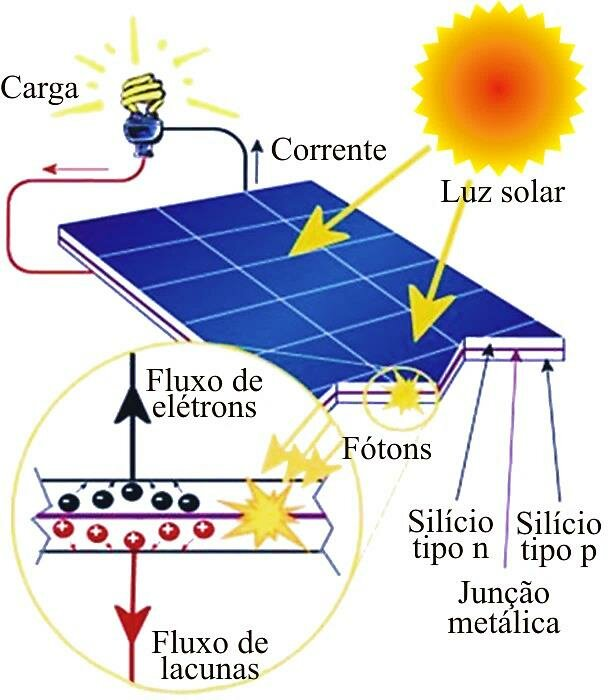
\includegraphics[width=0.70\textwidth]{Figuras/efeito_fotovoltaico.png}
\caption{Representação esquemática do efeito fotovoltaico em uma célula solar.}
\label{fig:efeito_fotovoltaico}
\fonte{Adaptado de Olivati (2001).}
\end{figure}

As células fotovoltaicas são interligadas eletricamente para formar os módulos fotovoltaicos, que constituem a unidade básica dos sistemas de geração de energia solar. O desempenho desses sistemas depende da capacidade dos módulos em converter a energia proveniente da radiação solar em energia elétrica útil. Entretanto, essa conversão é influenciada por diversos fatores, entre os quais destacam-se a irradiância solar, a temperatura de operação das células, o sombreamento, as características construtivas dos módulos, sua orientação, inclinação e o ângulo de incidência da radiação solar sobre sua superfície.

Segundo Veríssimo et al. (\citeyear{verissimo2017}), a incidência da radiação solar sobre os módulos fotovoltaicos exerce influência direta na geração de energia elétrica. Em sistemas convencionais, os painéis permanecem instalados em posição fixa, normalmente definida para maximizar a captação média anual de energia. Entretanto, como a posição aparente do Sol varia continuamente ao longo do dia, o ângulo de incidência da radiação modifica-se constantemente, fazendo com que os raios solares atinjam a superfície do painel em condições diferentes da orientação ideal durante grande parte do período de insolação.

Essa variação angular reduz a quantidade de radiação efetivamente aproveitada pelos módulos e, consequentemente, diminui a energia elétrica gerada. Dessa forma, parte das perdas observadas em sistemas fotovoltaicos não está associada apenas às características construtivas dos módulos, mas também às condições de posicionamento em relação ao Sol.

Além da orientação do painel, outros fatores também influenciam a eficiência energética do sistema, como o aumento da temperatura das células fotovoltaicas, o acúmulo de sujeira sobre os módulos, sombreamentos parciais, perdas elétricas em cabos e equipamentos de conversão de energia, bem como condições atmosféricas adversas. A atuação conjunta desses fatores pode reduzir significativamente o desempenho do sistema fotovoltaico.

Entre os fatores mencionados, a orientação do módulo em relação à radiação solar destaca-se por ser uma variável passível de controle por meio de sistemas de posicionamento automatizado. Conforme discutido por Veríssimo et al. (\citeyear{verissimo2017}), manter a incidência da radiação solar próxima da condição perpendicular ao painel favorece o aumento da energia captada, reduzindo perdas decorrentes da variação da posição aparente do Sol ao longo do dia.

Nesse contexto, a literatura apresenta diferentes estratégias para aumentar o aproveitamento energético dos sistemas fotovoltaicos, entre as quais se destacam os sistemas de rastreamento solar, responsáveis por ajustar continuamente a orientação dos módulos durante o período de operação. Os princípios de funcionamento desses sistemas serão apresentados na Seção~2.2.

%-----------------------------------
\section{Sistemas de Rastreamento Solar (Trackers)}

Embora seja a Terra que realize os movimentos de rotação e translação, para um observador localizado em sua superfície o Sol aparenta deslocar-se de leste para oeste ao longo do dia. Esse fenômeno, conhecido como movimento aparente do Sol, ocorre em decorrência da rotação terrestre. Além da variação diária, a trajetória aparente do Sol também se altera ao longo do ano devido à inclinação aproximada de 23,5° do eixo de rotação da Terra em relação ao plano de sua órbita, modificando a altura aparente do Sol e os ângulos de incidência da radiação solar sobre a superfície terrestre \cite{adolpho2024}.

A posição aparente do Sol pode ser descrita por dois parâmetros geométricos fundamentais: o ângulo de azimute solar e o ângulo de elevação solar. O ângulo de azimute representa a posição horizontal do Sol em relação aos pontos cardeais, enquanto o ângulo de elevação, também denominado altitude solar, corresponde à altura aparente do Sol acima da linha do horizonte. Esses parâmetros são amplamente utilizados na determinação da orientação de módulos fotovoltaicos e no desenvolvimento de sistemas de rastreamento solar, pois permitem estimar a direção de incidência da radiação solar ao longo do dia.

A Figura~\ref{fig:azimute} apresenta a geometria desses ângulos, ilustrando a relação entre a trajetória aparente do Sol, o ângulo de azimute e o ângulo de elevação.

\begin{figure}[H]
    \centering
    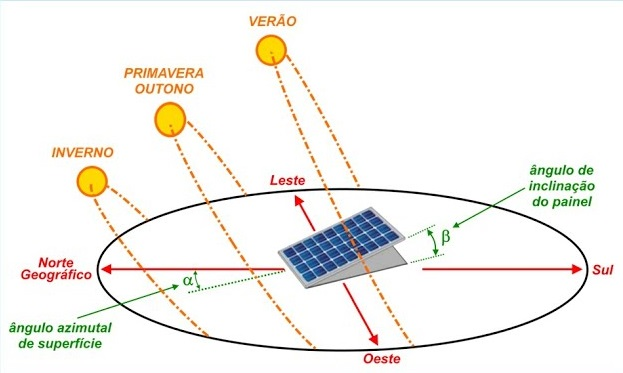
\includegraphics[width=0.75\textwidth]{Figuras/azimute_solar.jpg}
    \caption{Geometria solar ilustrando os ângulos de azimute e elevação solar.}
    \label{fig:azimute}
    \fonte{Adaptado de Adolpho Eletricista (2025).}
\end{figure}

O ângulo de azimute corresponde ao deslocamento horizontal da posição aparente do Sol em relação ao norte geográfico, sendo medido sobre o plano horizontal. Ao longo do dia, esse ângulo varia continuamente devido ao movimento aparente do Sol no sentido leste-oeste, sendo um parâmetro importante para definir a orientação horizontal de sistemas fotovoltaicos com rastreamento solar.

O ângulo de elevação solar corresponde ao ângulo formado entre a direção dos raios solares e o plano horizontal. Seu valor é aproximadamente igual a $0^\circ$ durante o nascer e o pôr do Sol, aumentando gradativamente ao longo da manhã até atingir o valor máximo nas proximidades do meio-dia solar, quando o Sol alcança sua maior altura aparente no céu. Em seguida, esse ângulo diminui progressivamente até retornar a aproximadamente $0^\circ$ no pôr do Sol.

Neste trabalho, esses conceitos são apresentados como fundamentação teórica para a compreensão do movimento aparente do Sol. Entretanto, o sistema desenvolvido utiliza como referência principal o horário para estimar a posição do painel fotovoltaico ao longo do dia, realizando posteriormente pequenos ajustes angulares com base na potência elétrica medida, sem efetuar o cálculo direto dos ângulos de azimute e elevação solar.

Na região Norte de Minas Gerais, situada aproximadamente na latitude de 16$^\circ$ Sul, observa-se elevada disponibilidade de radiação solar ao longo de praticamente todo o ano. Nessa região, a principal variação diária da posição aparente do Sol ocorre no sentido leste-oeste, associada à variação do ângulo de azimute, enquanto as alterações na elevação solar ao longo das estações do ano são relativamente menores quando comparadas às observadas em regiões de latitudes mais elevadas \cite{cemig2017}. Dessa forma, um sistema de rastreamento de eixo único, responsável por acompanhar o movimento diário do Sol no sentido leste-oeste, é capaz de proporcionar ganhos significativos na captação da radiação solar, justificando sua adoção neste trabalho.

O desempenho dos sistemas fotovoltaicos depende diretamente da quantidade de radiação solar incidente sobre a superfície dos módulos. Como os ângulos de azimute e elevação variam continuamente durante o dia e ao longo do ano, painéis instalados em posição fixa deixam de receber a radiação em condições próximas da perpendicularidade durante grande parte do período de insolação, reduzindo o aproveitamento da energia disponível.

Uma alternativa para minimizar essas perdas consiste na utilização de sistemas de rastreamento solar, também conhecidos como \textit{solar trackers}. Esses sistemas ajustam automaticamente a orientação dos módulos fotovoltaicos ao longo do dia, buscando manter a incidência da radiação solar em condições mais favoráveis e, consequentemente, aumentar a geração de energia elétrica \cite{verissimo2017}.

O princípio de funcionamento desses sistemas baseia-se no acompanhamento do movimento aparente do Sol. Esse acompanhamento pode ser realizado por diferentes estratégias, como sensores de luminosidade, modelos astronômicos baseados na posição solar ou algoritmos computacionais previamente programados. Independentemente da estratégia adotada, o objetivo permanece o mesmo: ajustar continuamente a posição do painel fotovoltaico para reduzir as perdas provocadas pela variação do ângulo de incidência da radiação solar.

Os sistemas de rastreamento podem ser classificados, de forma geral, em rastreadores de eixo único e rastreadores de dois eixos. Os rastreadores de eixo único realizam a movimentação do painel em apenas um plano, normalmente acompanhando o deslocamento do Sol no sentido leste-oeste. Em razão de sua construção mais simples, apresentam menor custo de implementação, menor consumo de energia para acionamento e menores exigências de manutenção quando comparados aos sistemas de dois eixos.

Por sua vez, os rastreadores de dois eixos permitem o movimento simultâneo em dois planos, acompanhando tanto a variação do azimute quanto da elevação solar ao longo do dia e das estações do ano. Essa configuração proporciona um alinhamento mais preciso entre o painel e a posição aparente do Sol, aumentando o aproveitamento da radiação incidente. Entretanto, apresenta maior complexidade mecânica, maior custo de fabricação, maior consumo de energia e maiores exigências de manutenção, fatores que podem limitar sua aplicação em sistemas fotovoltaicos de pequeno porte.

Diversos estudos têm demonstrado que a utilização de sistemas de rastreamento solar pode proporcionar ganhos significativos na geração de energia elétrica quando comparados aos sistemas convencionais de painel fixo. Entretanto, os resultados dependem da localização geográfica, das condições climáticas, da tecnologia empregada, do tipo de rastreador utilizado e da estratégia de controle adotada.

Nesse contexto, Almeida (\citeyear{almeida2024}) desenvolveu um sistema de rastreamento solar horizontal de eixo único utilizando o microcontrolador ESP32 como unidade de controle. O estudo propôs a substituição de controladores industriais por uma plataforma embarcada de menor custo, preservando as funcionalidades necessárias ao posicionamento automático do painel fotovoltaico. Os resultados experimentais demonstraram ganhos de geração de energia entre 17,51\% e 30,42\% em comparação com um sistema de painel fixo, indicando que rastreadores solares de eixo único representam uma alternativa tecnicamente viável para aplicações fotovoltaicas.

De forma semelhante, Moraes et al. (\citeyear{moraes2024}) avaliaram o desempenho de um sistema fotovoltaico equipado com rastreamento solar controlado por ESP32 em comparação com um sistema convencional de painel fixo. Os resultados evidenciaram um ganho energético aproximado de 37,9\%, atribuído ao melhor aproveitamento da radiação solar proporcionado pelo ajuste contínuo da orientação do painel. Além disso, o estudo destacou o potencial das plataformas embarcadas de baixo custo para o desenvolvimento de sistemas automatizados destinados à otimização da geração de energia fotovoltaica.

Os resultados apresentados nesses estudos demonstram que a utilização de rastreadores solares pode proporcionar ganhos significativos na geração de energia elétrica. Entretanto, o desempenho desses sistemas não depende apenas da estratégia de controle empregada, mas também da confiabilidade da estrutura eletromecânica responsável pelo posicionamento do painel. Motores, engrenagens e mecanismos de transmissão estão sujeitos a desgaste, desalinhamentos, falhas de acionamento e à ação de fatores ambientais, como vento, poeira e umidade. Essas condições podem comprometer o funcionamento do rastreador, mantendo o painel em posições desfavoráveis por longos períodos e reduzindo significativamente a geração de energia.

Além dos aspectos mecânicos, a confiabilidade operacional também está relacionada à arquitetura do sistema embarcado responsável pelo controle do rastreador. Sistemas baseados em microcontroladores permitem implementar algoritmos de posicionamento, controlar o acionamento dos atuadores, registrar dados de operação e integrar sensores para monitoramento do sistema. Essas funcionalidades contribuem para aumentar a robustez do sistema, reduzir movimentações desnecessárias e fornecer informações que podem ser utilizadas na identificação de falhas e na avaliação do desempenho operacional.

Nesse contexto, a utilização de modelos computacionais representa uma importante ferramenta para o desenvolvimento e a análise de sistemas de rastreamento solar. As simulações permitem avaliar diferentes estratégias de controle, estimar o comportamento do sistema em condições variadas de operação e prever seu desempenho antes da implementação física. Entretanto, para que esses modelos possam ser utilizados com confiabilidade, torna-se necessária sua validação por meio da comparação entre resultados simulados e dados experimentais obtidos em sistemas reais. Os fundamentos relacionados à modelagem e à simulação computacional são apresentados na Seção~2.4.

%-----------------------------------
\section{Sistemas Embarcados}


Os sistemas embarcados são sistemas computacionais desenvolvidos para executar funções específicas de monitoramento, controle e processamento de informações em dispositivos eletrônicos. Diferentemente dos computadores de propósito geral, esses sistemas são projetados para desempenhar tarefas dedicadas, normalmente operando em tempo real e sob restrições de processamento, consumo de energia, memória e custo de implementação.

Segundo Chase e Almeida (\citeyear{chase2007}), um sistema embarcado caracteriza-se pela integração entre hardware e software, sendo projetado para executar funções específicas. Nesse contexto, o software embarcado processa informações provenientes de sensores, executa algoritmos de controle e aciona atuadores, permitindo que o sistema responda automaticamente às condições observadas no ambiente.

De forma geral, a arquitetura de um sistema embarcado é composta por sensores responsáveis pela aquisição de dados do ambiente, um microcontrolador encarregado do processamento dessas informações e atuadores que executam as ações determinadas pelo algoritmo de controle. A Figura~\ref{fig:embarcado} apresenta, de forma simplificada, o funcionamento básico de um sistema embarcado, destacando a interação entre o ambiente, os dispositivos de entrada e saída e a unidade de processamento.

\begin{figure}[H]
    \centering
    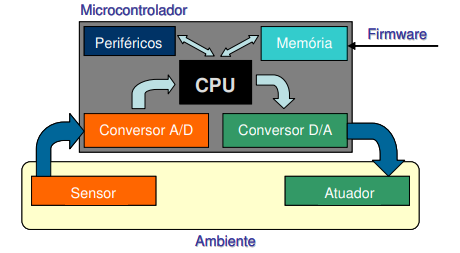
\includegraphics[width=0.85\textwidth]{Figuras/sistemas_embarcados.png}
    \caption{Diagrama básico de um sistema embarcado dotado de um microcontrolador monitorando o ambiente.}
    \label{fig:embarcado}
    \fonte{Adaptado de Chase e Almeida (2007).}
\end{figure}

Essa arquitetura é amplamente empregada em aplicações de automação industrial, robótica, Internet das Coisas (IoT), sistemas automotivos e monitoramento remoto. No contexto deste trabalho, esse modelo é aplicado ao sistema fotovoltaico automatizado, no qual o microcontrolador realiza a aquisição de dados provenientes dos sensores, processa as informações e controla o posicionamento do painel fotovoltaico por meio de um atuador.

O microcontrolador constitui o elemento central dessa arquitetura, sendo responsável pela execução do algoritmo de controle, pela leitura dos sinais provenientes dos sensores e pelo acionamento dos dispositivos de saída. Dessa forma, integra aquisição de dados, processamento e tomada de decisão em tempo real, permitindo que o sistema opere de maneira autônoma e responda às condições de funcionamento previamente estabelecidas.

Diversas plataformas baseadas em microcontroladores são empregadas no desenvolvimento de sistemas embarcados, destacando-se dispositivos das famílias PIC, AVR, ESP32, STM32 e Raspberry Pi Pico. A escolha da plataforma depende dos requisitos da aplicação, considerando fatores como capacidade de processamento, memória disponível, número de entradas e saídas, interfaces de comunicação, consumo de energia e custo de implementação.

Para aplicações de automação em sistemas fotovoltaicos de pequeno porte, plataformas baseadas na arquitetura AVR, como o Arduino Uno, apresentam capacidade computacional suficiente para executar algoritmos de controle, realizar a aquisição de dados provenientes de sensores e acionar dispositivos eletromecânicos. Além disso, a ampla disponibilidade de bibliotecas, interfaces de comunicação e módulos compatíveis favorece sua utilização em pesquisas experimentais e no desenvolvimento de protótipos acadêmicos \cite{arduino2023}.

Os sensores constituem a interface entre o ambiente físico e o sistema computacional, convertendo grandezas físicas em sinais elétricos interpretáveis pelo microcontrolador. Em sistemas fotovoltaicos, esses dispositivos permitem monitorar continuamente variáveis como tensão, corrente, temperatura e irradiância, fornecendo informações essenciais para a avaliação do desempenho energético e para a implementação de estratégias de controle.

Os atuadores são responsáveis por converter os comandos emitidos pelo sistema de controle em ações físicas sobre o processo monitorado. Em sistemas fotovoltaicos automatizados, essa função consiste em movimentar mecanicamente o painel fotovoltaico conforme a estratégia de posicionamento definida pelo algoritmo de controle. Entre os dispositivos mais utilizados em aplicações experimentais destacam-se os servomotores, que permitem o controle preciso da posição angular por meio de sinais PWM (\textit{Pulse Width Modulation}), apresentando boa precisão de posicionamento, simplicidade de integração e reduzida complexidade de controle \cite{arduino2023} .

Além dos elementos principais, sistemas embarcados frequentemente incorporam módulos auxiliares destinados ao armazenamento de dados, sincronização temporal e interface com o usuário. Dispositivos como módulos de cartão SD, relógios de tempo real (RTC) e displays permitem registrar informações experimentais, manter a referência temporal das medições e acompanhar o funcionamento do sistema durante sua operação.

A integração entre sensores, microcontroladores, atuadores e módulos auxiliares constitui a base dos sistemas embarcados modernos, possibilitando a aquisição contínua de dados, o processamento em tempo real, o controle automático de processos físicos e o armazenamento das informações produzidas. Essas características tornam essa arquitetura adequada para aplicações de automação, monitoramento e controle, incluindo sistemas fotovoltaicos automatizados.
%-----------------------------------
\section{Modelagem e Simulação de Sistemas}

A modelagem computacional consiste na representação matemática de sistemas físicos com o objetivo de descrever e prever seu comportamento por meio de modelos capazes de reproduzir, de forma aproximada, os fenômenos observados na realidade. Associada à simulação computacional, essa abordagem permite analisar diferentes condições de operação sem a necessidade da construção imediata de protótipos físicos, reduzindo tempo, custos de desenvolvimento e riscos experimentais \cite{dvorak2023}.

Segundo Melo (\citeyear{melo2019}), a determinação da posição aparente do Sol por meio de parâmetros astronômicos constitui a base para modelos computacionais empregados na simulação do desempenho de sistemas fotovoltaicos. Esses modelos possibilitam estimar o comportamento do sistema sob diferentes condições de operação, servindo como ferramenta de apoio ao projeto e à análise de desempenho.

Entre as ferramentas utilizadas para modelagem de sistemas destaca-se o \textit{MATrix LABoratory} (MATLAB) e seu ambiente de simulação Simulink, amplamente empregados em aplicações de engenharia devido à disponibilidade de bibliotecas para modelagem matemática, processamento numérico e simulação de sistemas dinâmicos. O Simulink permite representar modelos por meio de diagramas de blocos, facilitando a implementação de sistemas de controle e a análise do comportamento de processos físicos \cite{mathworks_simulink}.

Neste trabalho foi adotado como ponto de partida o modelo computacional disponibilizado por Nagi (\citeyear{nagi2023}), implementado no ambiente MATLAB/Simulink para comparação entre sistemas fotovoltaicos com painel fixo e com rastreamento solar. O modelo foi adaptado para representar as características do sistema automatizado desenvolvido nesta pesquisa e posteriormente validado por meio da comparação entre os resultados simulados e os dados experimentais obtidos com o protótipo físico.

Embora a modelagem computacional permita analisar previamente o comportamento do sistema, sua confiabilidade depende da capacidade do modelo em representar adequadamente o sistema físico. Dessa forma, a validação experimental constitui uma etapa essencial do processo de modelagem, sendo realizada por meio da comparação entre os resultados simulados e os dados obtidos experimentalmente em condições equivalentes de operação \cite{dvorak2023}. Essa comparação permite verificar a representatividade do modelo computacional em relação ao comportamento observado na prática, aumentando sua confiabilidade para análises e estudos futuros.

A utilização conjunta da modelagem computacional e da experimentação física constitui uma estratégia importante para o desenvolvimento de sistemas fotovoltaicos automatizados. Enquanto o modelo computacional possibilita prever o comportamento esperado do sistema em diferentes condições de operação, os ensaios experimentais permitem verificar sua representatividade em condições reais. Dessa forma, a comparação entre simulação e experimento fornece evidências sobre a validade do modelo computacional e amplia sua confiabilidade como ferramenta de apoio ao desenvolvimento e à avaliação de sistemas fotovoltaicos automatizados.
\chapter{Metodologia}

Este capítulo apresenta os procedimentos metodológicos adotados para o desenvolvimento, implementação e avaliação do sistema fotovoltaico automatizado proposto neste trabalho. A pesquisa possui abordagem quantitativa, sendo conduzida por meio do desenvolvimento de um protótipo experimental e da comparação entre resultados obtidos por simulação computacional e dados experimentais coletados em condições reais de operação.

metodologia foi estruturada de forma a contemplar todas as etapas necessárias para o desenvolvimento e a validação do sistema proposto. A metodologia foi estruturada em quatro etapas principais: seleção dos materiais e construção do protótipo experimental; desenvolvimento da lógica de funcionamento do sistema; modelagem computacional no ambiente MATLAB/Simulink; e realização dos ensaios experimentais para validação do modelo computacional.

Após a implementação do protótipo, foram realizados ensaios experimentais em ambiente externo, sob condições reais de operação, utilizando simultaneamente um sistema automatizado e um sistema com painel fixo como referência. Durante os experimentos, foram registradas as variáveis elétricas necessárias para a avaliação do desempenho dos dois sistemas. Os dados experimentais obtidos durante os ensaios foram organizados, processados e comparados aos resultados gerados pelo modelo computacional desenvolvido no MATLAB/Simulink. 

Essa comparação permitiu avaliar a capacidade do modelo em representar o comportamento observado no protótipo físico, validando sua utilização como ferramenta de apoio para a análise do desempenho do sistema fotovoltaico automatizado. A Figura~\ref{fig:fluxo_metodologia} apresenta, de forma resumida, as principais etapas que compõem a metodologia adotada neste trabalho.

\begin{figure}[H]
    \centering
    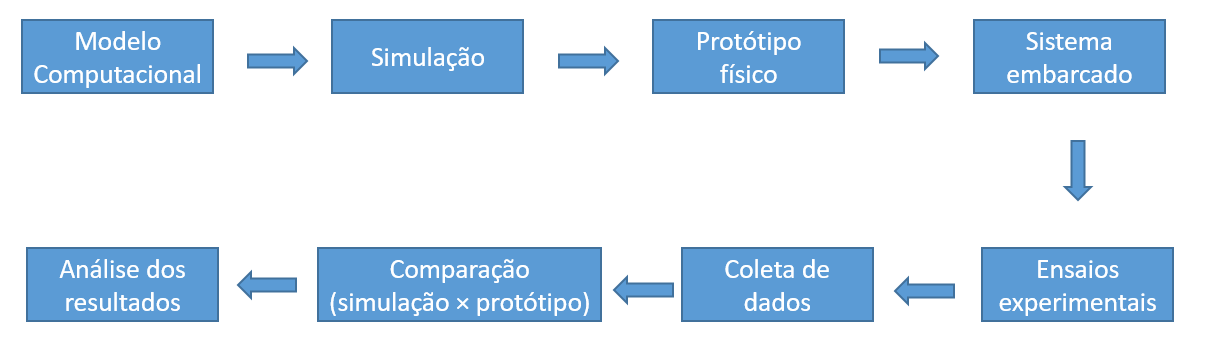
\includegraphics[width=0.95\textwidth]{Figuras/fluxo_metodologia}
    \caption{Fluxograma das etapas metodológicas desenvolvidas neste trabalho.}
    \label{fig:fluxo_metodologia}
    \fonte{Elaborado pelo autor.}
\end{figure}

As seções seguintes descrevem detalhadamente os materiais empregados, a arquitetura de hardware e software do sistema, o desenvolvimento do modelo computacional, os procedimentos experimentais adotados e os métodos utilizados para análise e comparação dos resultados.

\section{Materiais e Hardware}

    \subsection{Painel Fotovoltaico}

O protótipo experimental foi desenvolvido utilizando um módulo fotovoltaico policristalino com potência nominal de 3~W, tensão nominal de 6~V em corrente contínua e dimensões aproximadas de 21~cm $\times$ 13~cm, conforme apresentado na Figura~\ref{fig:placa_solar}. A escolha desse módulo deve-se à sua compatibilidade com a proposta experimental, permitindo a realização de ensaios comparativos entre um sistema automatizado e um sistema de painel fixo com baixo custo de implementação.

\begin{figure}[H]
    \centering
    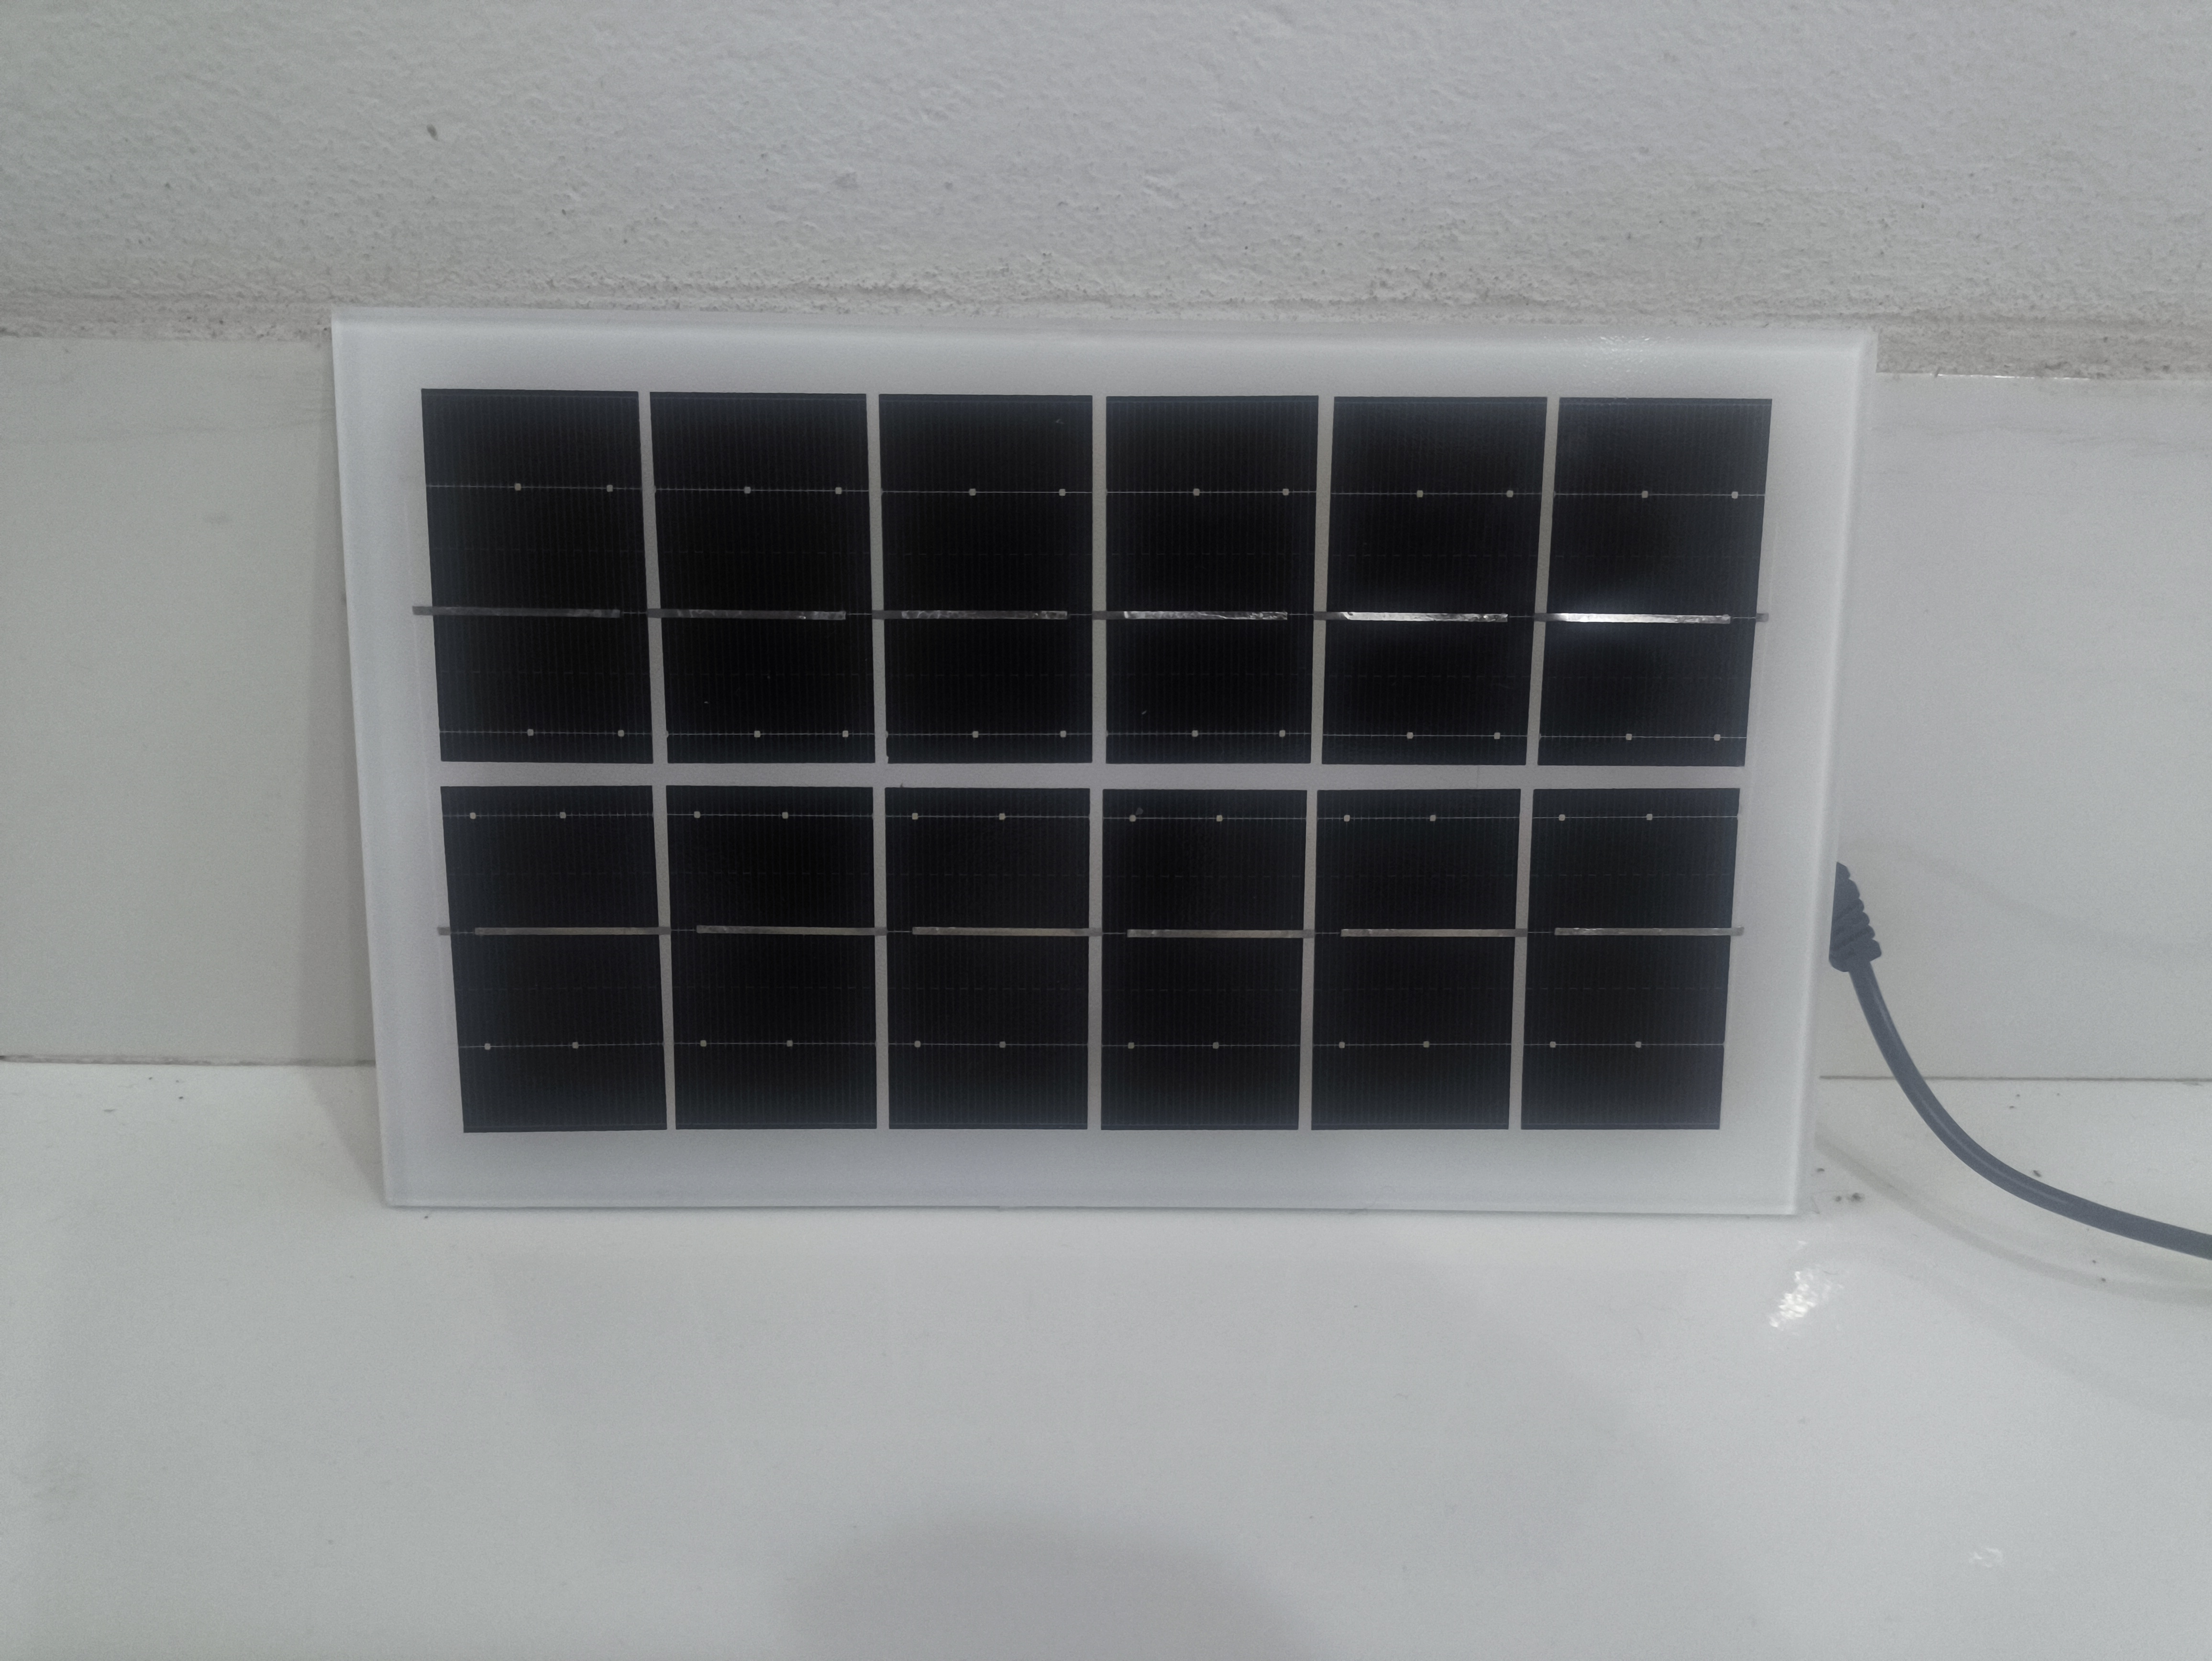
\includegraphics[width=0.7\textwidth]{Figuras/placa_solar.jpg}
    \caption{Painel fotovoltaico utilizado no protótipo experimental.}
    \label{fig:placa_solar}
    \fonte{Autor (2026).}
\end{figure}

O painel fotovoltaico constituiu o elemento responsável pela conversão da radiação solar em energia elétrica e pela geração das variáveis elétricas monitoradas durante os experimentos. As medições de tensão e corrente obtidas por meio dos sensores instalados no sistema foram utilizadas para o cálculo da potência elétrica instantânea e para a comparação do desempenho entre o sistema automatizado e o sistema com painel fixo.

Embora apresente potência reduzida quando comparado aos módulos empregados em instalações comerciais, o painel utilizado possui características suficientes para aplicações experimentais, permitindo reproduzir o comportamento de sistemas fotovoltaicos de maior porte em escala reduzida. Essa abordagem é frequentemente adotada em pesquisas experimentais por possibilitar a avaliação de estratégias de controle e posicionamento com menor custo e maior facilidade de implementação.

Para possibilitar uma comparação direta entre as duas configurações avaliadas, foram utilizados dois painéis fotovoltaicos com as mesmas especificações durante os experimentos. Um permaneceu em posição fixa, enquanto o outro foi acoplado ao mecanismo automatizado de movimentação, possibilitando a comparação direta entre as duas configurações sob as mesmas condições ambientais.

As especificações técnicas dos módulos foram fornecidas pelo fabricante considerando as Condições Padrão de Teste (\textit{Standard Test Conditions} -- STC), conforme estabelecido pela norma IEC 61215. Nessas condições, os painéis operam próximos de sua potência nominal \cite{iec2016}.

Durante os experimentos, os módulos foram instalados em ambiente externo e submetidos às condições reais de operação, nas quais a irradiância solar e a temperatura das células variam continuamente ao longo do dia. Dessa forma, os valores obtidos representam o comportamento dos sistemas em condições reais de funcionamento, permitindo avaliar a influência do posicionamento automatizado sobre a geração de energia elétrica.

\subsection{Microcontrolador Arduino}

A unidade de processamento do protótipo foi implementada utilizando a plataforma Arduino Uno, baseada no microcontrolador ATmega328P. A placa opera a 16 MHz, possui 14 portas digitais de entrada e saída, das quais seis podem operar como saídas PWM (\textit{Pulse Width Modulation}), além de seis entradas analógicas destinadas à aquisição de sinais provenientes de sensores \cite{arduino2023}. A placa utilizada é apresentada na Figura~\ref{fig:arduino_uno}. 
\begin{figure}[H]
    \centering
    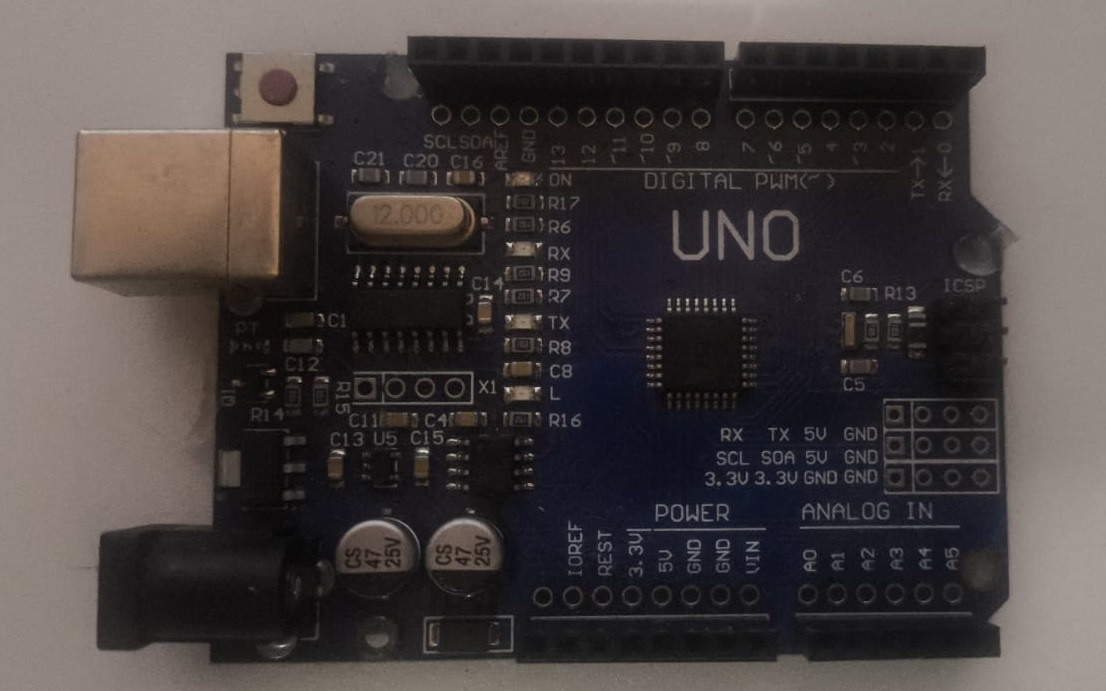
\includegraphics[width=0.6\textwidth]{Figuras/Placa Arduino Uno.jpeg}
    \caption{Placa Arduino Uno utilizada no protótipo.}
    \label{fig:arduino_uno}
    \fonte{Autor (2026).}
\end{figure}

A escolha dessa plataforma foi motivada por sua capacidade de atender aos requisitos computacionais do sistema desenvolvido, que envolvem aquisição de dados, processamento em tempo real, controle de atuadores e comunicação com dispositivos periféricos. Além disso, a disponibilidade de interfaces digitais, entradas analógicas e bibliotecas específicas simplifica a integração com sensores, servomotores, módulos RTC, display LCD e dispositivos de armazenamento em cartão SD.

No protótipo desenvolvido, o Arduino Uno atuou como unidade central de controle, executando continuamente o algoritmo responsável pelo monitoramento e pelo posicionamento automatizado do painel fotovoltaico. Durante a operação do sistema, o microcontrolador realiza a leitura dos sensores de tensão e corrente, calcula a potência elétrica instantânea a partir dessas medições, determina o ângulo de posicionamento do painel com base no horário fornecido pelo módulo RTC, aciona o servomotor por meio de sinais PWM, atualiza as informações exibidas no display LCD e registra automaticamente os dados experimentais no cartão microSD para posterior análise.

Dessa forma, o Arduino Uno atuou como elemento central do sistema embarcado, coordenando todas as etapas de monitoramento, controle e registro das informações experimentais. A lógica de funcionamento implementada no microcontrolador é apresentada na Seção~3.2.

\subsection{Servomotor}

O acionamento mecânico do painel fotovoltaico foi realizado por meio de um servomotor modelo MG996R, apresentado na Figura~\ref{fig:servo_mg996r}. A escolha desse dispositivo deve-se ao seu elevado torque, à boa precisão de posicionamento angular e à facilidade de integração com a plataforma Arduino, características adequadas para aplicações de controle de posição em sistemas automatizados.

\begin{figure}[H]
    \centering
    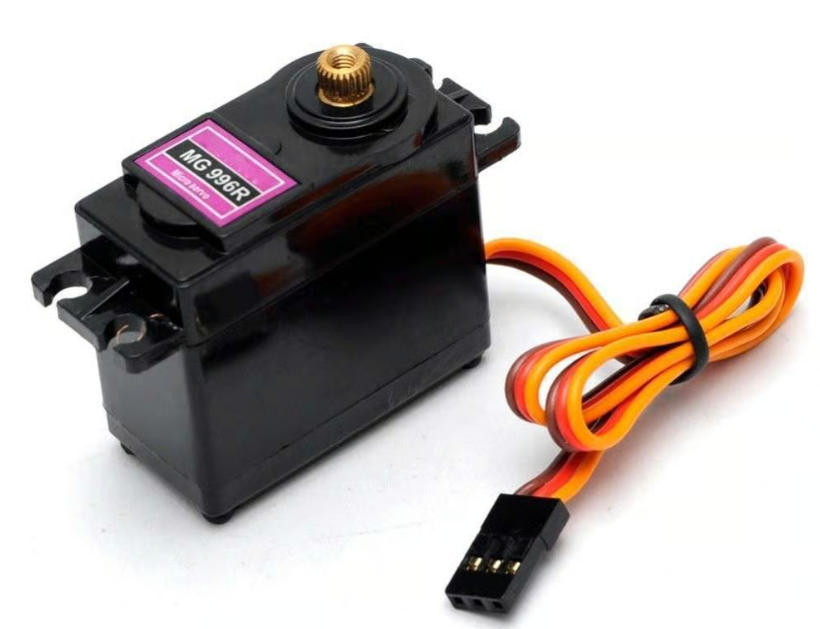
\includegraphics[width=0.6\textwidth]{Figuras/servo motor.png}
    \caption{Servomotor MG996R utilizado no protótipo.}
    \label{fig:servo_mg996r}
    \fonte{Adaptado de Eletrônica Castro (2026).}
\end{figure}

O servomotor MG996R possui faixa de operação aproximada de 0° a 180° e realiza o posicionamento angular a partir de sinais PWM (\textit{Pulse Width Modulation}) enviados pelo microcontrolador. Essa característica proporciona boa precisão e repetibilidade dos movimentos, tornando o dispositivo adequado para aplicações de controle de posição em sistemas automatizados \cite{towerpro2019,arduino_servo}.

No sistema desenvolvido, o servomotor foi responsável pelo posicionamento automático do painel fotovoltaico ao longo do período de operação. O ângulo de rotação foi determinado pelo algoritmo implementado no Arduino com base no horário fornecido pelo módulo RTC, realizando o deslocamento gradual do painel entre as posições correspondentes ao nascer e ao pôr do Sol.

Considerando que o posicionamento do painel influencia diretamente a incidência da radiação solar sobre sua superfície, A utilização do servomotor possibilitou implementar o controle automático da posição angular do painel fotovoltaico sem a necessidade de mecanismos adicionais de posicionamento, contribuindo para simplificar a construção do protótipo e reduzir sua complexidade mecânica e eletrônica.


\subsection{Sensores de Corrente e Tensão}

A aquisição das variáveis elétricas do sistema foi realizada por meio de um sensor de corrente ACS712 e de um módulo sensor de tensão baseado em divisor resistivo, apresentados na Figura~\ref{fig:sensores}. Esses dispositivos foram utilizados para monitorar continuamente a corrente e a tensão produzidas pelo painel fotovoltaico durante os ensaios experimentais, fornecendo as informações necessárias para o cálculo da potência elétrica gerada.

\begin{figure}[H]
    \centering

    \begin{minipage}{0.45\linewidth}
        \centering
        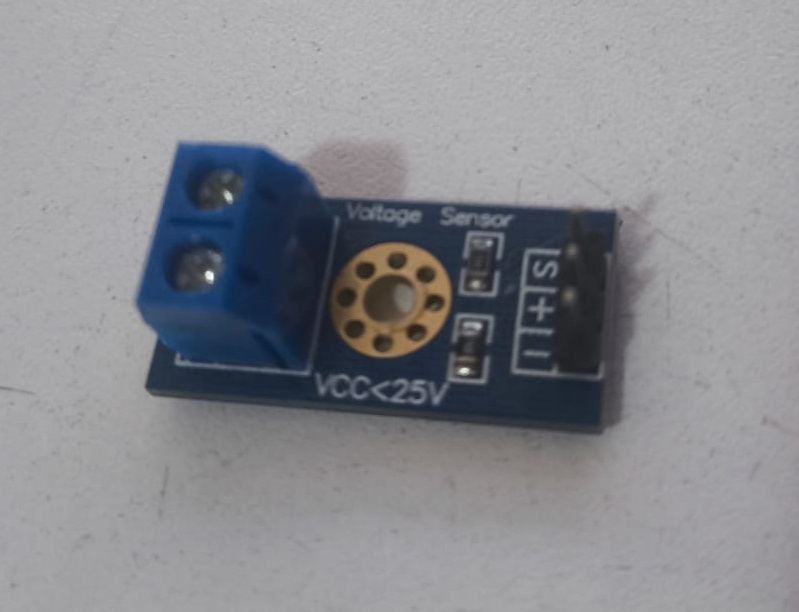
\includegraphics[height=5cm]{Figuras/sensor_tensao.jpeg}

        (a) Sensor de tensão
    \end{minipage}
    \hfill
    \begin{minipage}{0.45\linewidth}
        \centering
        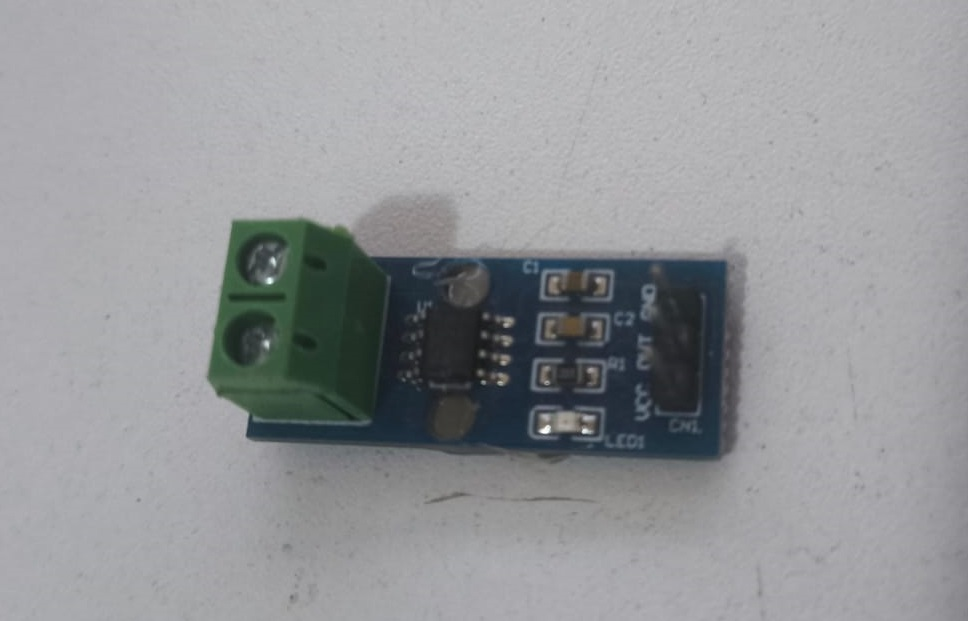
\includegraphics[height=5cm]{Figuras/sensor_corrente.jpeg}

        (b) Sensor de corrente
    \end{minipage}

    \caption{Sensores utilizados para aquisição das grandezas elétricas do sistema.}
    \label{fig:sensores}
    \fonte{Autor (2026).}
\end{figure}

O sensor ACS712, baseado no efeito Hall, realiza a medição indireta da corrente elétrica, disponibilizando ao microcontrolador um sinal analógico proporcional à corrente que circula no circuito, preservando o isolamento elétrico entre o circuito de potência e o circuito de medição \cite{allegro2019,sparkfun_acs712}. O módulo sensor de tensão, por sua vez, utiliza um divisor resistivo para reduzir a tensão aplicada à sua entrada para níveis compatíveis com as entradas analógicas do Arduino, permitindo a medição segura de tensões contínuas de até 25~V \cite{usinainfo2024,sedra2016}.

Os sinais analógicos provenientes dos dois sensores foram adquiridos pelo conversor analógico-digital do Arduino e convertidos em valores de tensão e corrente por meio das rotinas de calibração implementadas no software de controle. A partir dessas grandezas foi calculada, em tempo real, a potência elétrica instantânea produzida pelo painel fotovoltaico, utilizando a Equação~\ref{eq:potencia}.

\begin{equation}
P = V \times I
\label{eq:potencia}
\end{equation}

em que $P$ representa a potência elétrica (W), $V$ corresponde à tensão elétrica (V) e $I$ representa a corrente elétrica (A).

As medições foram realizadas automaticamente em intervalos de um minuto durante todo o período experimental, compreendido entre 06h00 e 18h00. Esse intervalo de aquisição foi adotado para permitir o acompanhamento da variação das grandezas elétricas ao longo do dia e o cálculo da energia acumulada produzida pelos sistemas.

As variáveis elétricas calculadas foram utilizadas para o monitoramento do desempenho do sistema, sendo apresentadas em tempo real no display LCD e registradas automaticamente no cartão microSD, juntamente com a data, o horário e o ângulo de posicionamento do painel fotovoltaico. Posteriormente, esses dados constituíram a base para a análise do desempenho energético do sistema, permitindo a comparação entre o sistema automatizado e o sistema de painel fixo, bem como a validação do modelo computacional desenvolvido no ambiente MATLAB/Simulink.

\subsection{Módulo RTC DS1307}

O controle temporal do sistema foi realizado por meio do módulo \textit{Real-Time Clock} (RTC) DS1307, apresentado na Figura~\ref{fig:rtc}. Esse dispositivo foi utilizado para fornecer informações de data e horário durante a operação do protótipo, permitindo sincronizar o funcionamento do sistema e registrar cronologicamente os dados experimentais coletados.

\begin{figure}[H]
    \centering
    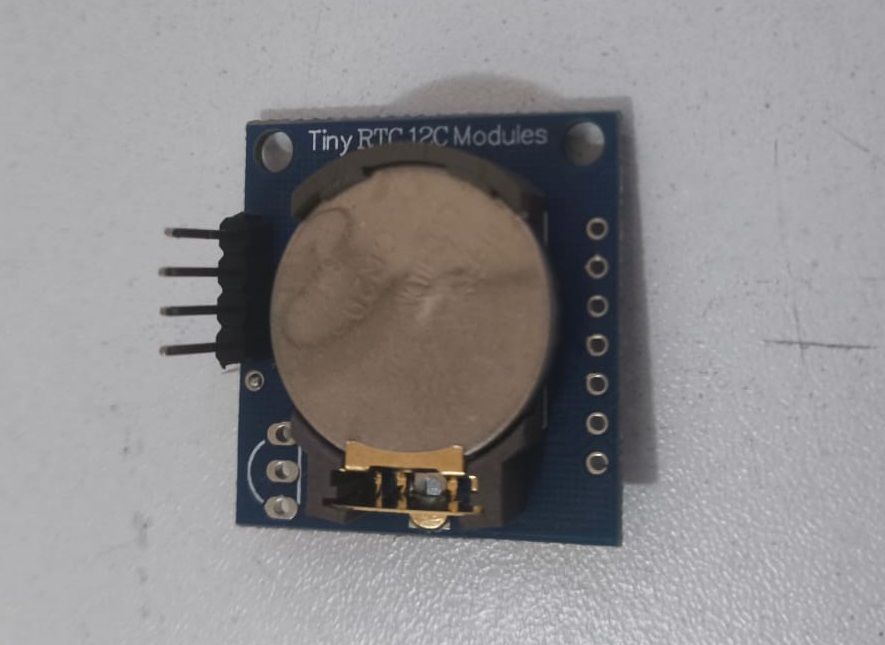
\includegraphics[width=0.6\textwidth]{Figuras/rtc.jpeg}
    \caption{Módulo RTC DS1307 utilizado no protótipo.}
    \label{fig:rtc}
    \fonte{Autor (2026).}
\end{figure}

O DS1307 comunica-se com o Arduino por meio do protocolo I\textsuperscript{2}C, utilizando as linhas SDA e SCL para troca de dados. O módulo possui bateria de backup, responsável por manter a contagem de data e hora mesmo na ausência de alimentação elétrica, preservando as informações temporais armazenadas \cite{maxim2015}.

No sistema desenvolvido, o RTC desempenhou duas funções principais. A primeira foi fornecer a referência temporal utilizada pelo algoritmo de controle para determinar o posicionamento angular do painel fotovoltaico ao longo do dia. A segunda consistiu em registrar a data e o horário correspondentes a cada medição de tensão, corrente e potência armazenada no cartão microSD, permitindo organizar os dados experimentais em ordem cronológica.

A utilização do módulo RTC garantiu a sincronização entre o controle do posicionamento do painel e a aquisição das grandezas elétricas, contribuindo para a consistência dos dados utilizados na comparação entre o sistema automatizado, o sistema de painel fixo e o modelo computacional desenvolvido neste trabalho.

\subsection{Display de Cristal Líquido (Liquid Crystal Display -- LCD)}

Para a interface entre o sistema embarcado e o usuário, foi utilizado um display LCD 16$\times$2 com interface I2C, apresentado na Figura~\ref{fig:lcd}. Esse dispositivo permite a exibição de caracteres alfanuméricos distribuídos em duas linhas de 16 colunas e é amplamente empregado em sistemas embarcados devido ao seu baixo custo, reduzido consumo de energia e facilidade de integração com microcontroladores \cite{makerhero2022}.

\begin{figure}[H]
    \centering
    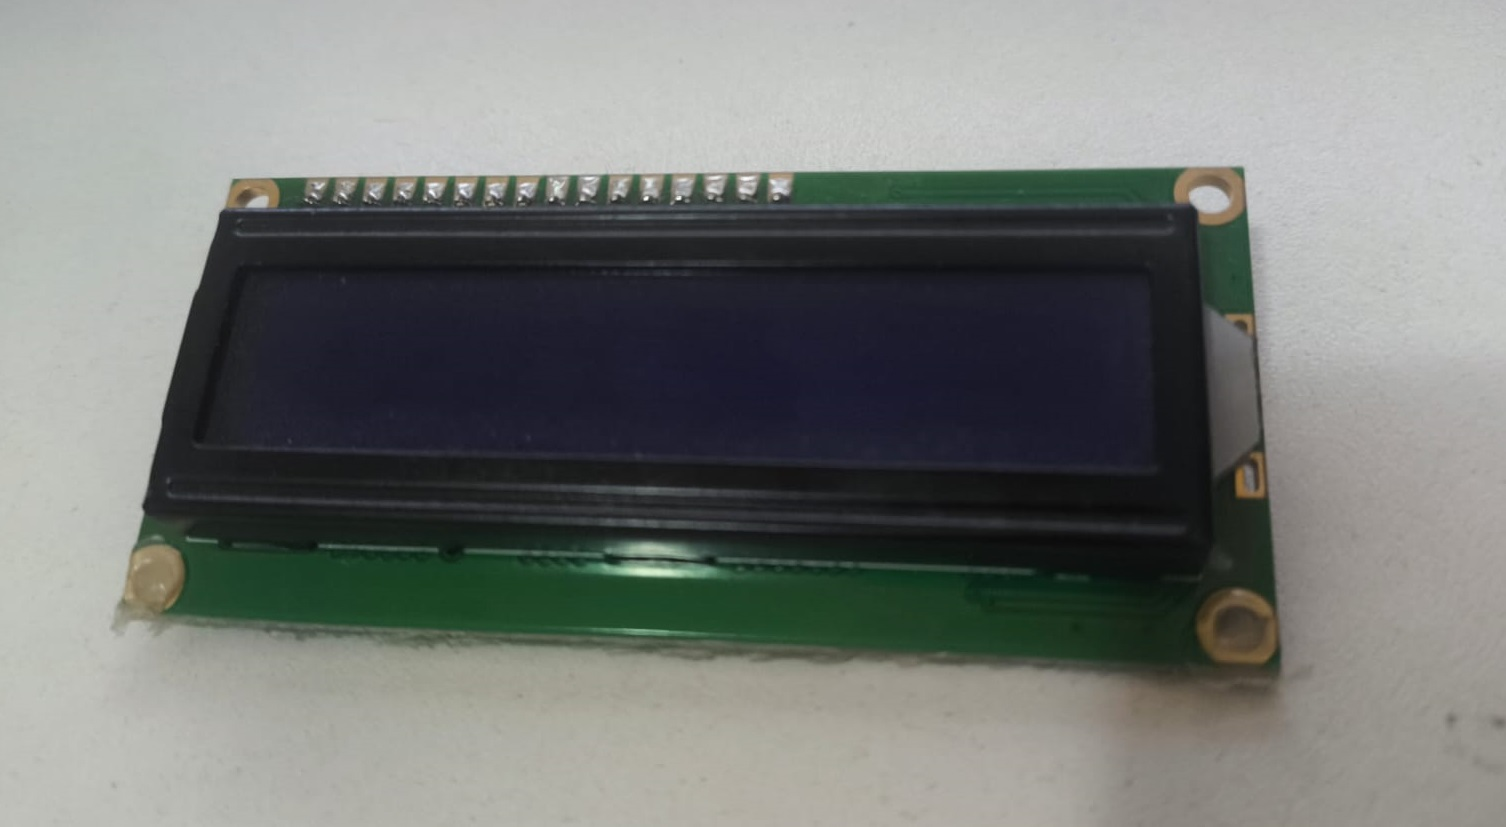
\includegraphics[width=0.6\textwidth]{Figuras/display.jpeg}
    \caption{Display LCD 16$\times$2 com interface I2C utilizado no sistema.}
    \label{fig:lcd}
    \fonte{Autor (2026).}
\end{figure}

A comunicação entre o display e o Arduino é realizada por meio do protocolo I2C, utilizando apenas as linhas SDA e SCL. Essa característica reduz a quantidade de conexões necessárias em relação à interface paralela convencional, simplificando a montagem do circuito e liberando portas de entrada e saída do microcontrolador para outras funções do sistema.

Durante a operação do protótipo, o display apresenta em tempo real as principais informações monitoradas pelo sistema, incluindo data e horário fornecidos pelo módulo RTC, tensão elétrica (V), corrente elétrica (I), potência instantânea (P) e o ângulo de posicionamento do painel fotovoltaico. Essas informações permitiram acompanhar continuamente o funcionamento do sistema durante os ensaios experimentais.

Além da exibição das variáveis elétricas, o display também foi utilizado para apresentar mensagens relacionadas ao estado de funcionamento do sistema, auxiliando no monitoramento da operação do protótipo durante a aquisição dos dados experimentais.

\subsection{Módulo Leitor de Cartão Micro SD}

Para o armazenamento dos dados experimentais foi utilizado um módulo leitor de cartão microSD, apresentado na Figura~\ref{fig:sd}. Esse dispositivo permite registrar automaticamente as informações adquiridas pelo sistema durante os ensaios, possibilitando sua utilização nas etapas de tratamento, análise e comparação dos resultados.

\begin{figure}[H]
    \centering
    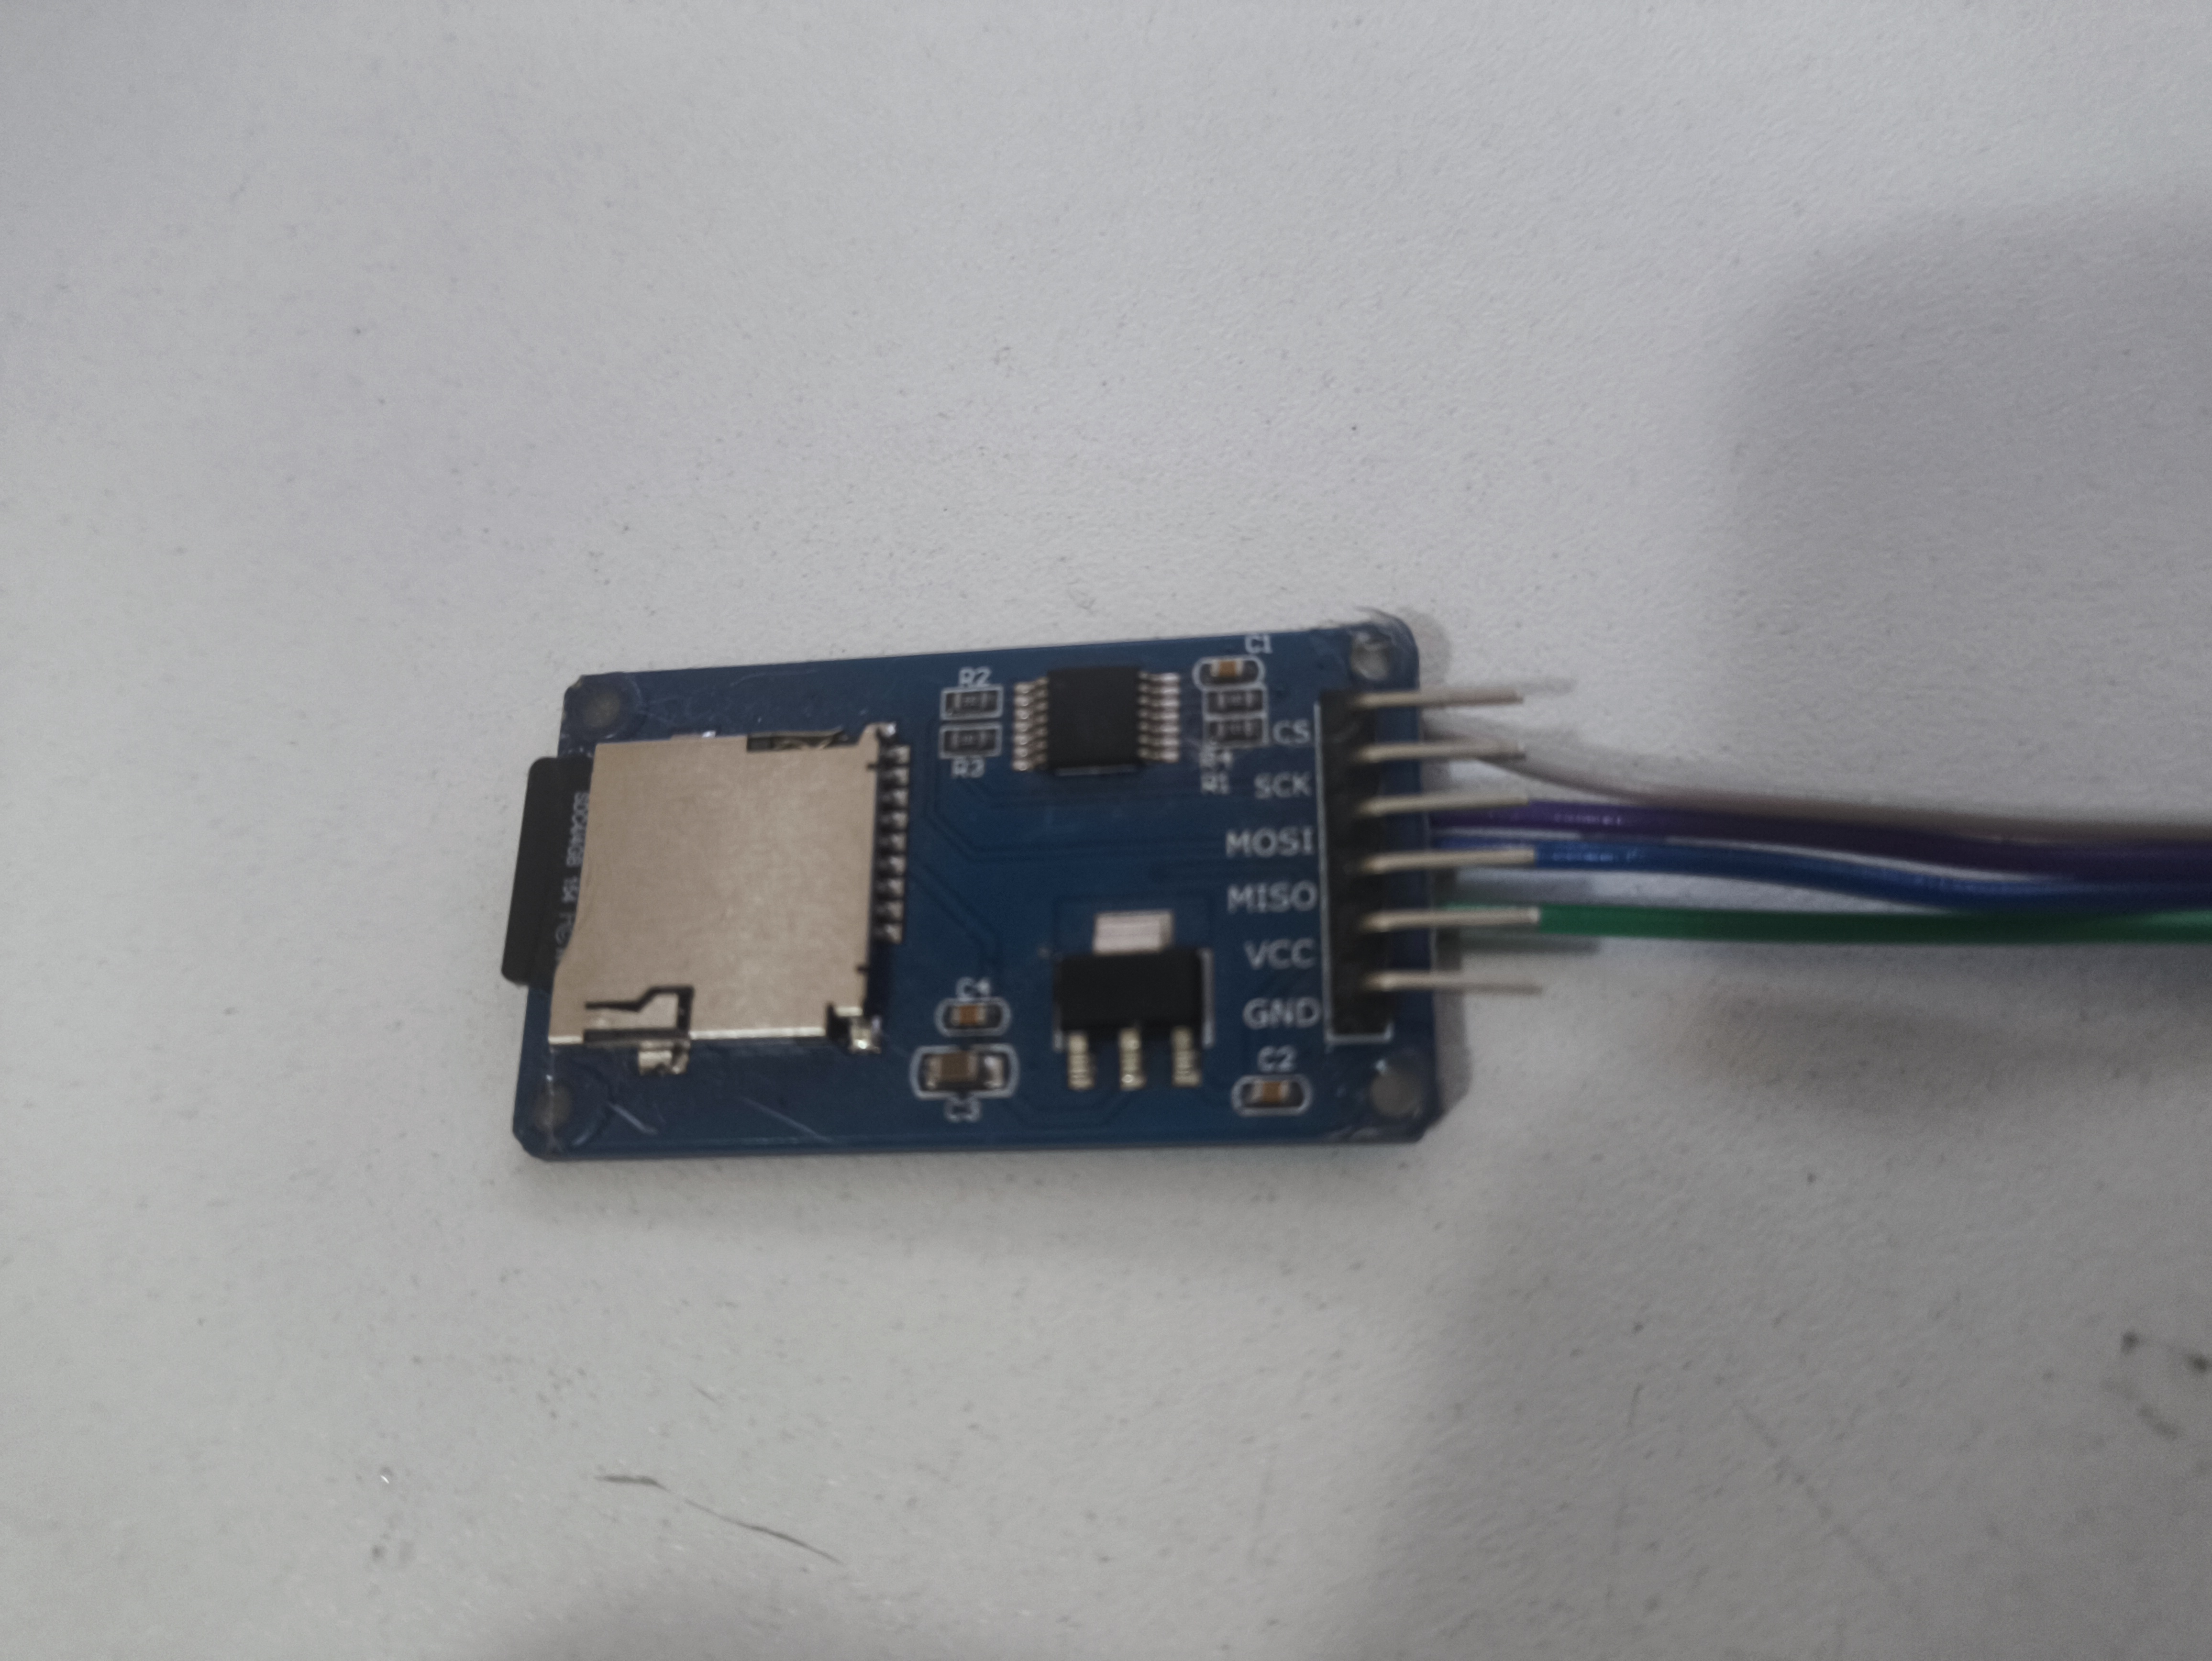
\includegraphics[width=0.6\textwidth]{Figuras/cartao_sd.jpg}
    \caption{Módulo leitor de cartão microSD utilizado no sistema.}
    \label{fig:sd}
    \fonte{Autor (2026).}
\end{figure}

O módulo comunica-se com o Arduino por meio da interface SPI (\textit{Serial Peripheral Interface}), permitindo operações de leitura e escrita em cartões de memória microSD. Essa solução é amplamente utilizada em sistemas embarcados que necessitam registrar dados durante longos períodos de operação, possibilitando o armazenamento organizado das informações em arquivos digitais compatíveis com softwares de planilhas eletrônicas e ferramentas de análise de dados \cite{eletrogate2022}.

No protótipo desenvolvido, foram registrados automaticamente a data, o horário, a tensão elétrica, a corrente elétrica, a potência instantânea e o ângulo de posicionamento do painel fotovoltaico. O registro cronológico dessas informações permitiu a construção das séries temporais utilizadas na comparação entre o sistema automatizado e o sistema de painel fixo.

Após a realização dos experimentos, os arquivos foram importados para planilhas eletrônicas, onde os dados foram organizados e processados para obtenção dos gráficos, tabelas e indicadores utilizados na análise dos resultados.

Dessa forma, o módulo leitor de cartão microSD desempenhou papel fundamental no sistema de aquisição de dados, garantindo o registro organizado das informações experimentais e fornecendo suporte às etapas de processamento, análise e validação dos resultados obtidos.

\subsection{Arquitetura do Sistema}

A arquitetura do protótipo foi desenvolvida para possibilitar a aquisição de dados experimentais destinados à validação do modelo computacional e à comparação do desempenho entre um sistema fotovoltaico automatizado e um sistema de painel fixo. Dessa forma, o protótipo constitui uma ferramenta de pesquisa destinada à aquisição de dados experimentais, não representando um sistema projetado para aplicação comercial ou operação contínua em ambientes externos.

A estrutura do protótipo foi construída utilizando uma base de madeira e componentes mecânicos fabricados por impressão 3D em filamento PLA, incluindo o suporte do painel fotovoltaico e o conjunto de engrenagens responsável pela transmissão do movimento. A opção por esses materiais deve-se ao baixo custo e à facilidade de fabricação, características adequadas ao desenvolvimento de protótipos acadêmicos. Entretanto, reconhece-se que os materiais apresentam limitações quanto à resistência mecânica e à durabilidade quando expostos continuamente às condições ambientais, como radiação ultravioleta, variações de temperatura e intempéries. Assim, o protótipo foi concebido exclusivamente para a realização dos testes experimentais previstos neste trabalho.

A movimentação do painel fotovoltaico é realizada por um servomotor MG996R acoplado ao conjunto de engrenagens impressas em PLA, permitindo a rotação do painel em torno de um único eixo no sentido leste-oeste. Essa configuração reproduz o princípio de funcionamento de um sistema de rastreamento solar de eixo único, sendo suficiente para os experimentos realizados. Como o objetivo deste trabalho consiste na validação do modelo computacional por meio de dados experimentais, não foram avaliados aspectos relacionados à resistência mecânica ou à viabilidade construtiva do protótipo.

As Figuras~\ref{fig:engrenagem1} e~\ref{fig:engrenagem2} apresentam o suporte estrutural e o conjunto de engrenagens utilizados no sistema de transmissão mecânica.

\begin{figure}[H]
    \centering
    \begin{minipage}{0.45\linewidth}
        \centering
        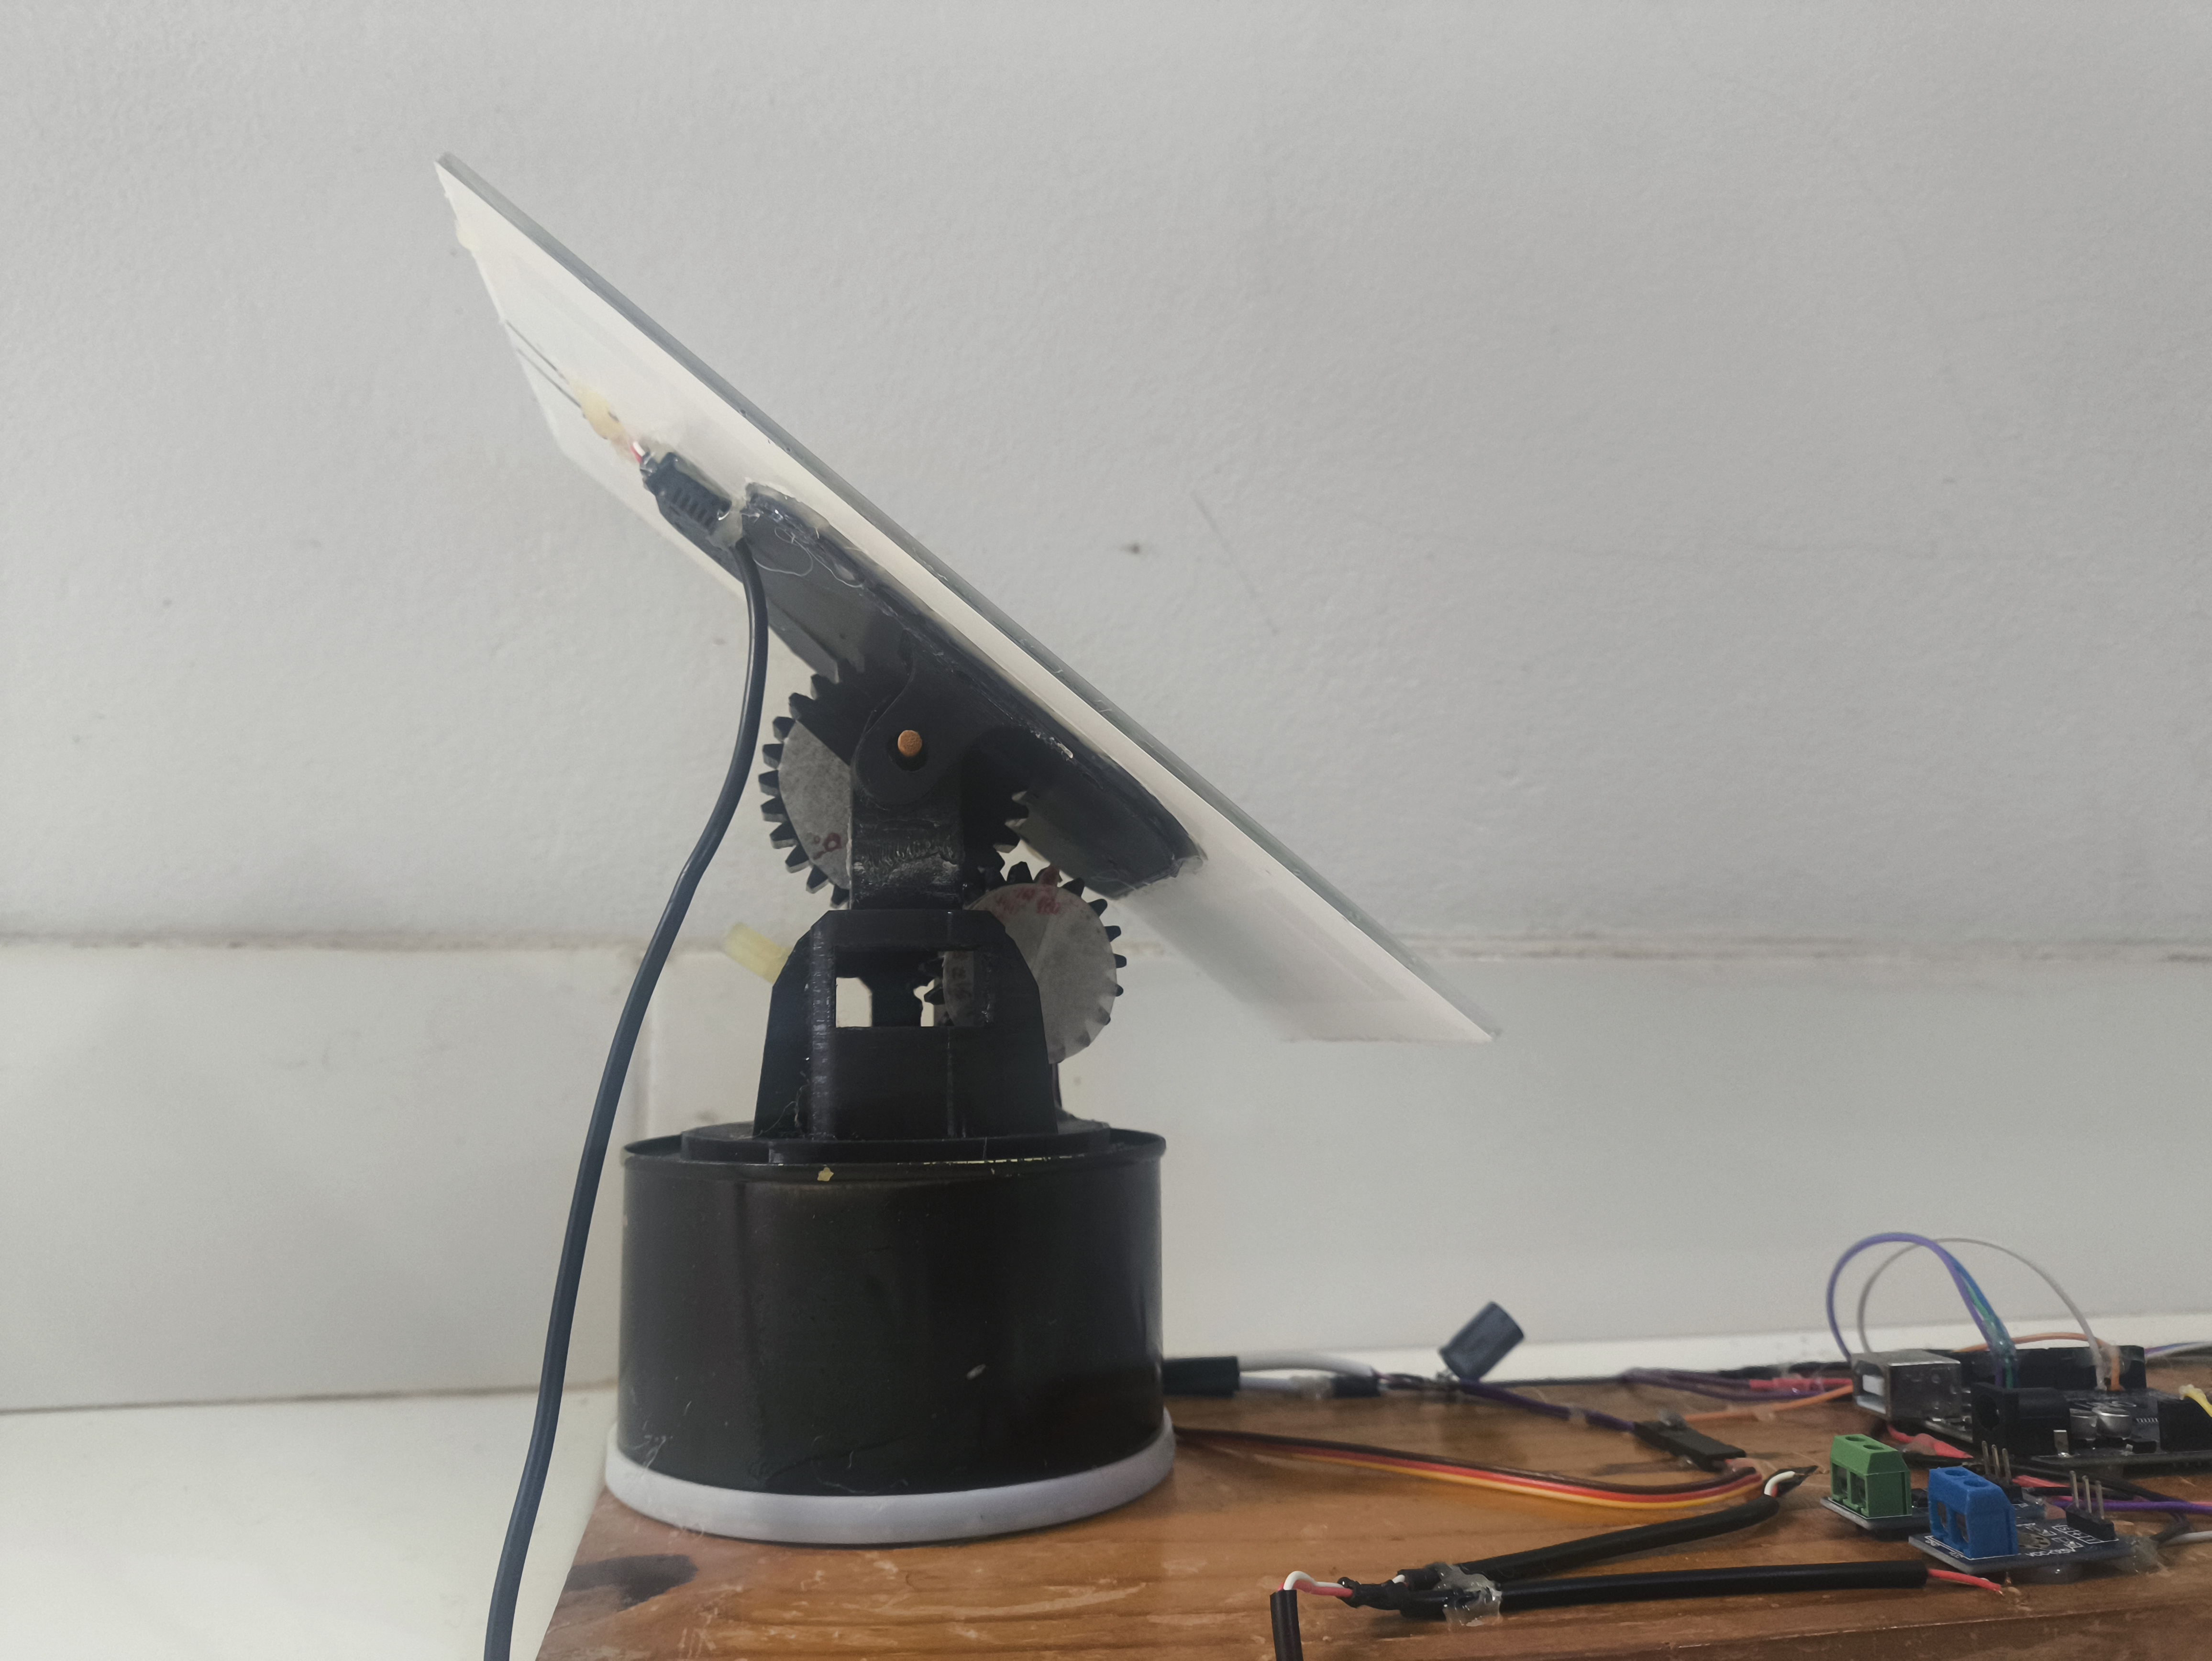
\includegraphics[width=\linewidth]{Figuras/engrenagem1.jpg}
        \caption{Suporte e engrenagem produzidos por impressão 3D.}
        \label{fig:engrenagem1}
        \fonte{Autor (2026).}
    \end{minipage}
    \hfill
    \begin{minipage}{0.45\linewidth}
        \centering
        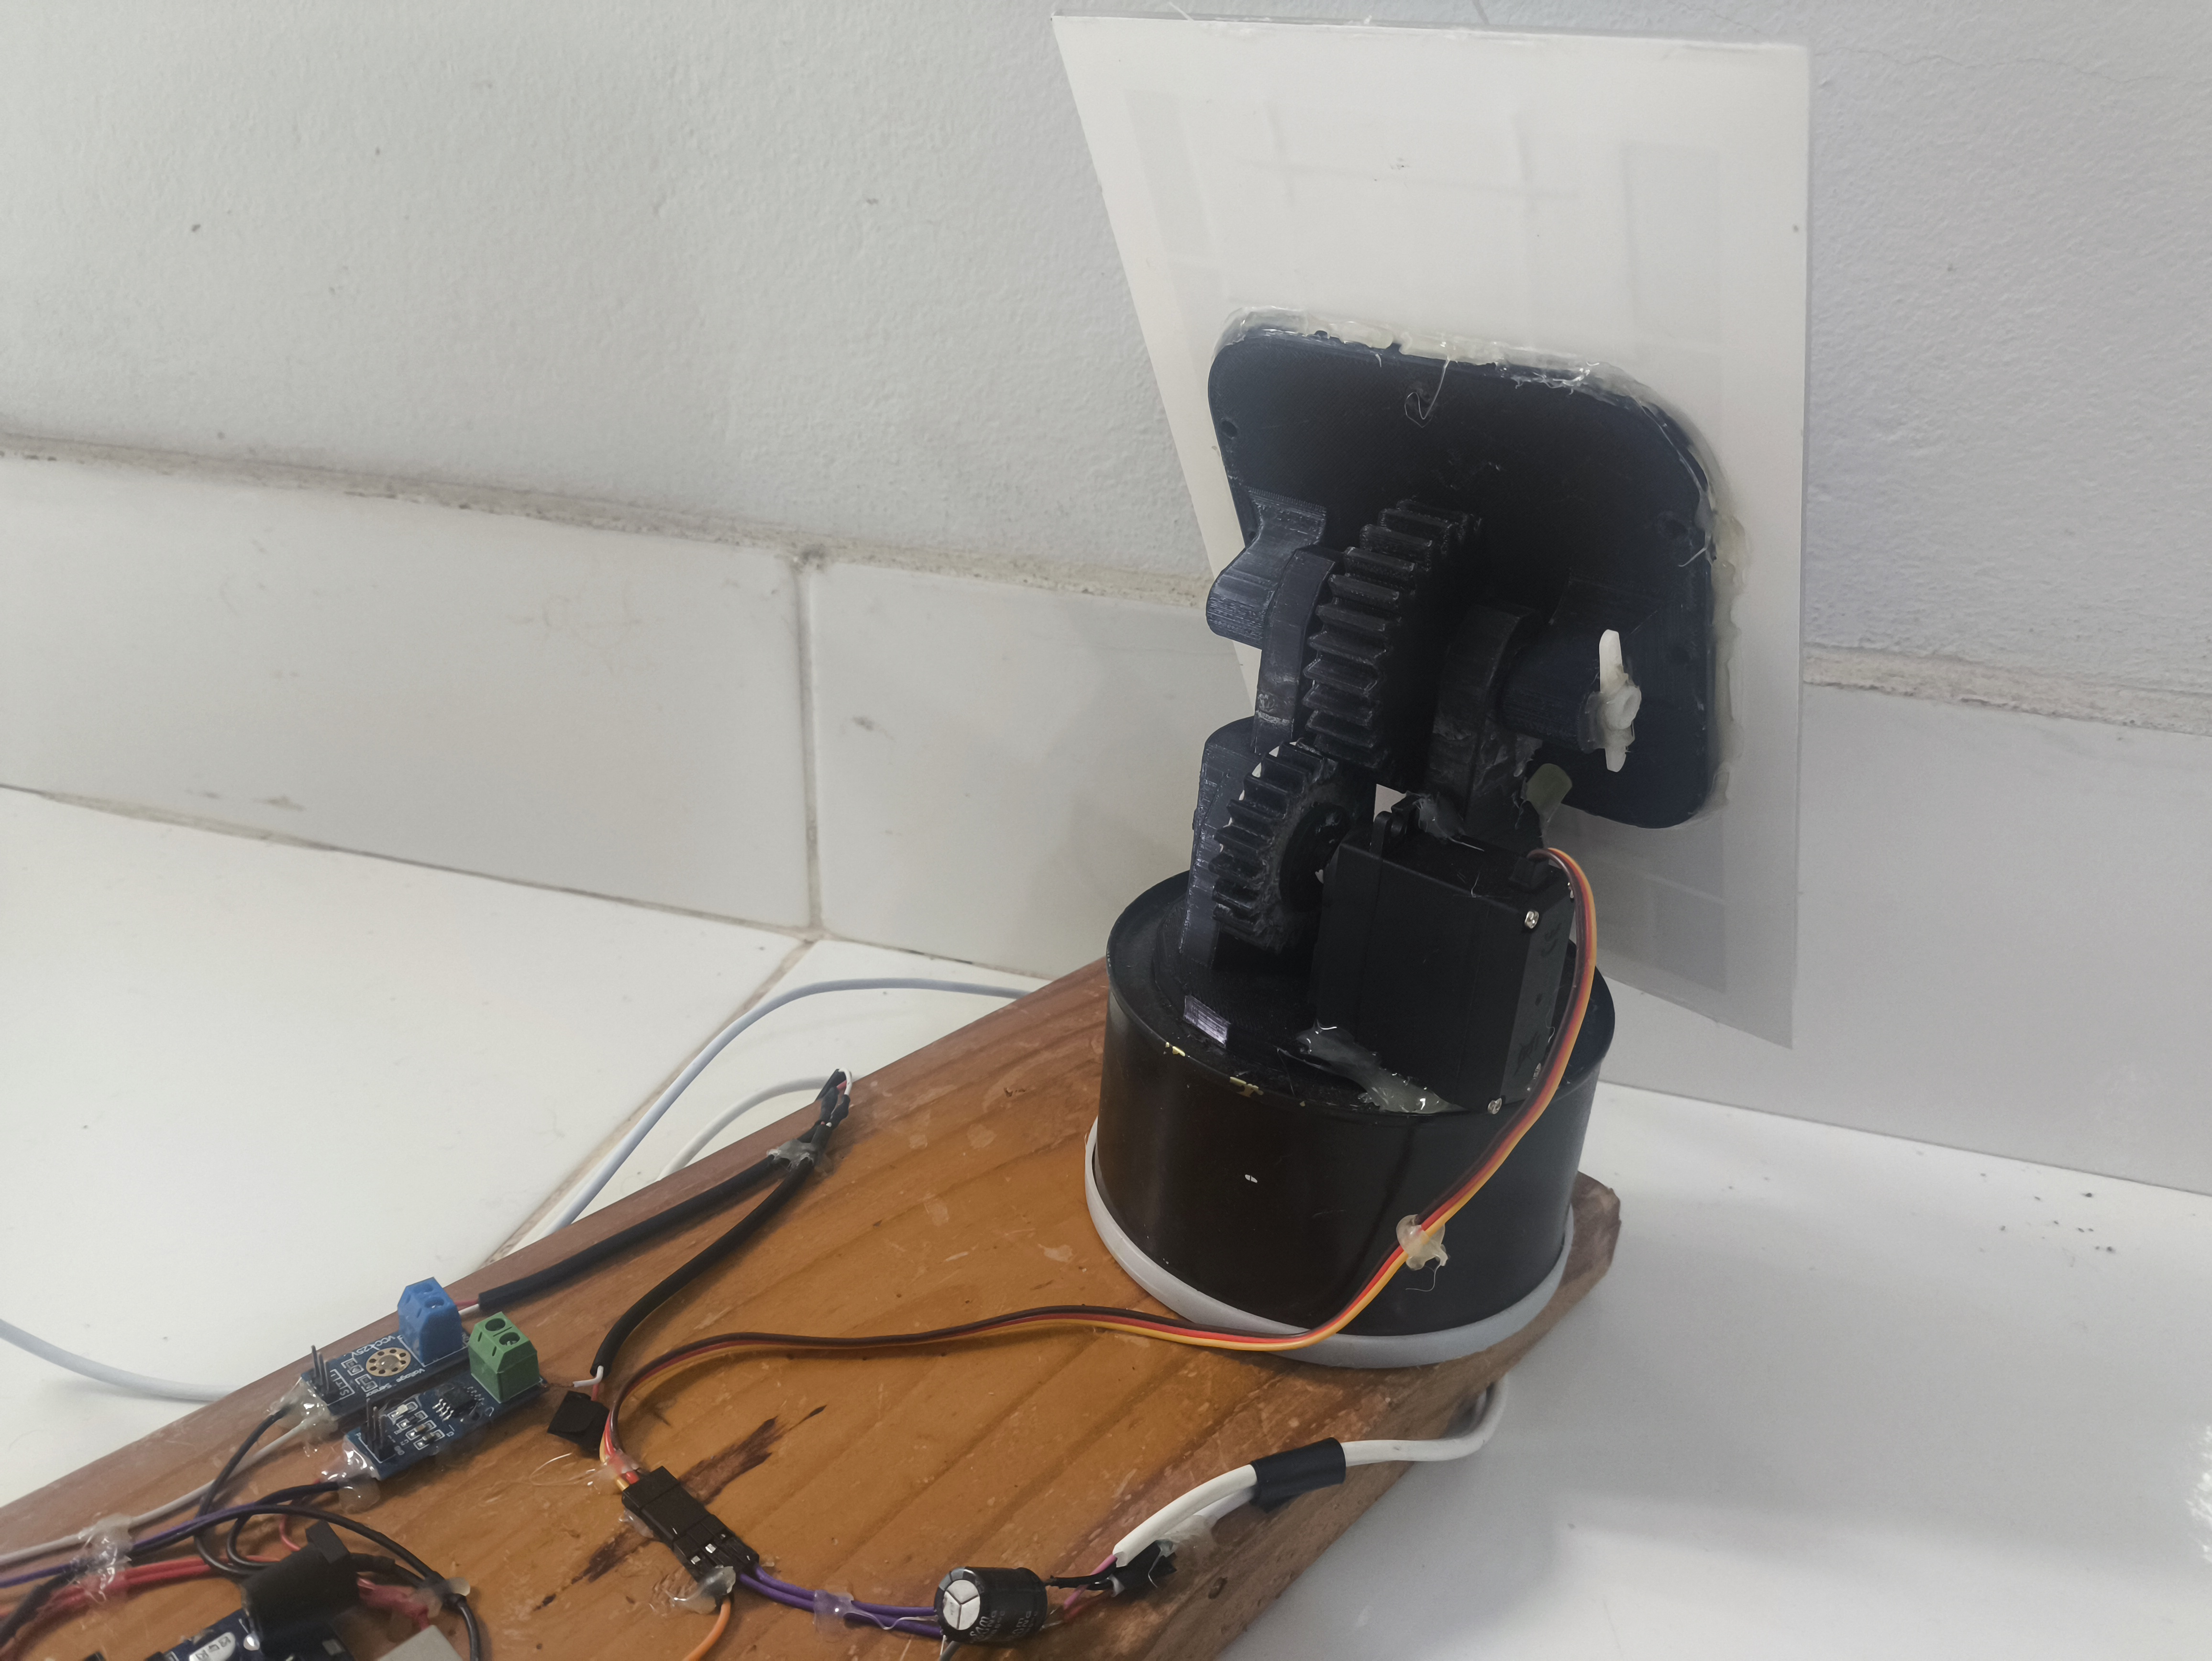
\includegraphics[width=\linewidth]{Figuras/engrenagem2.jpg}
        \caption{Detalhamento do conjunto de transmissão mecânica.}
        \label{fig:engrenagem2}
        \fonte{Autor (2026).}
    \end{minipage}
\end{figure}

Os componentes eletrônicos, incluindo o Arduino Uno, os sensores, o módulo RTC, o display LCD e o módulo leitor de cartão microSD, foram organizados sobre a base estrutural de forma a facilitar a montagem, a manutenção e a organização das conexões elétricas, contribuindo para a confiabilidade durante os ensaios experimentais.

A Figura~\ref{fig:prototipo_montado} apresenta o protótipo completamente montado, evidenciando a integração entre a estrutura mecânica, o sistema de acionamento e os módulos eletrônicos utilizados no desenvolvimento do trabalho.

\begin{figure}[H]
    \centering
    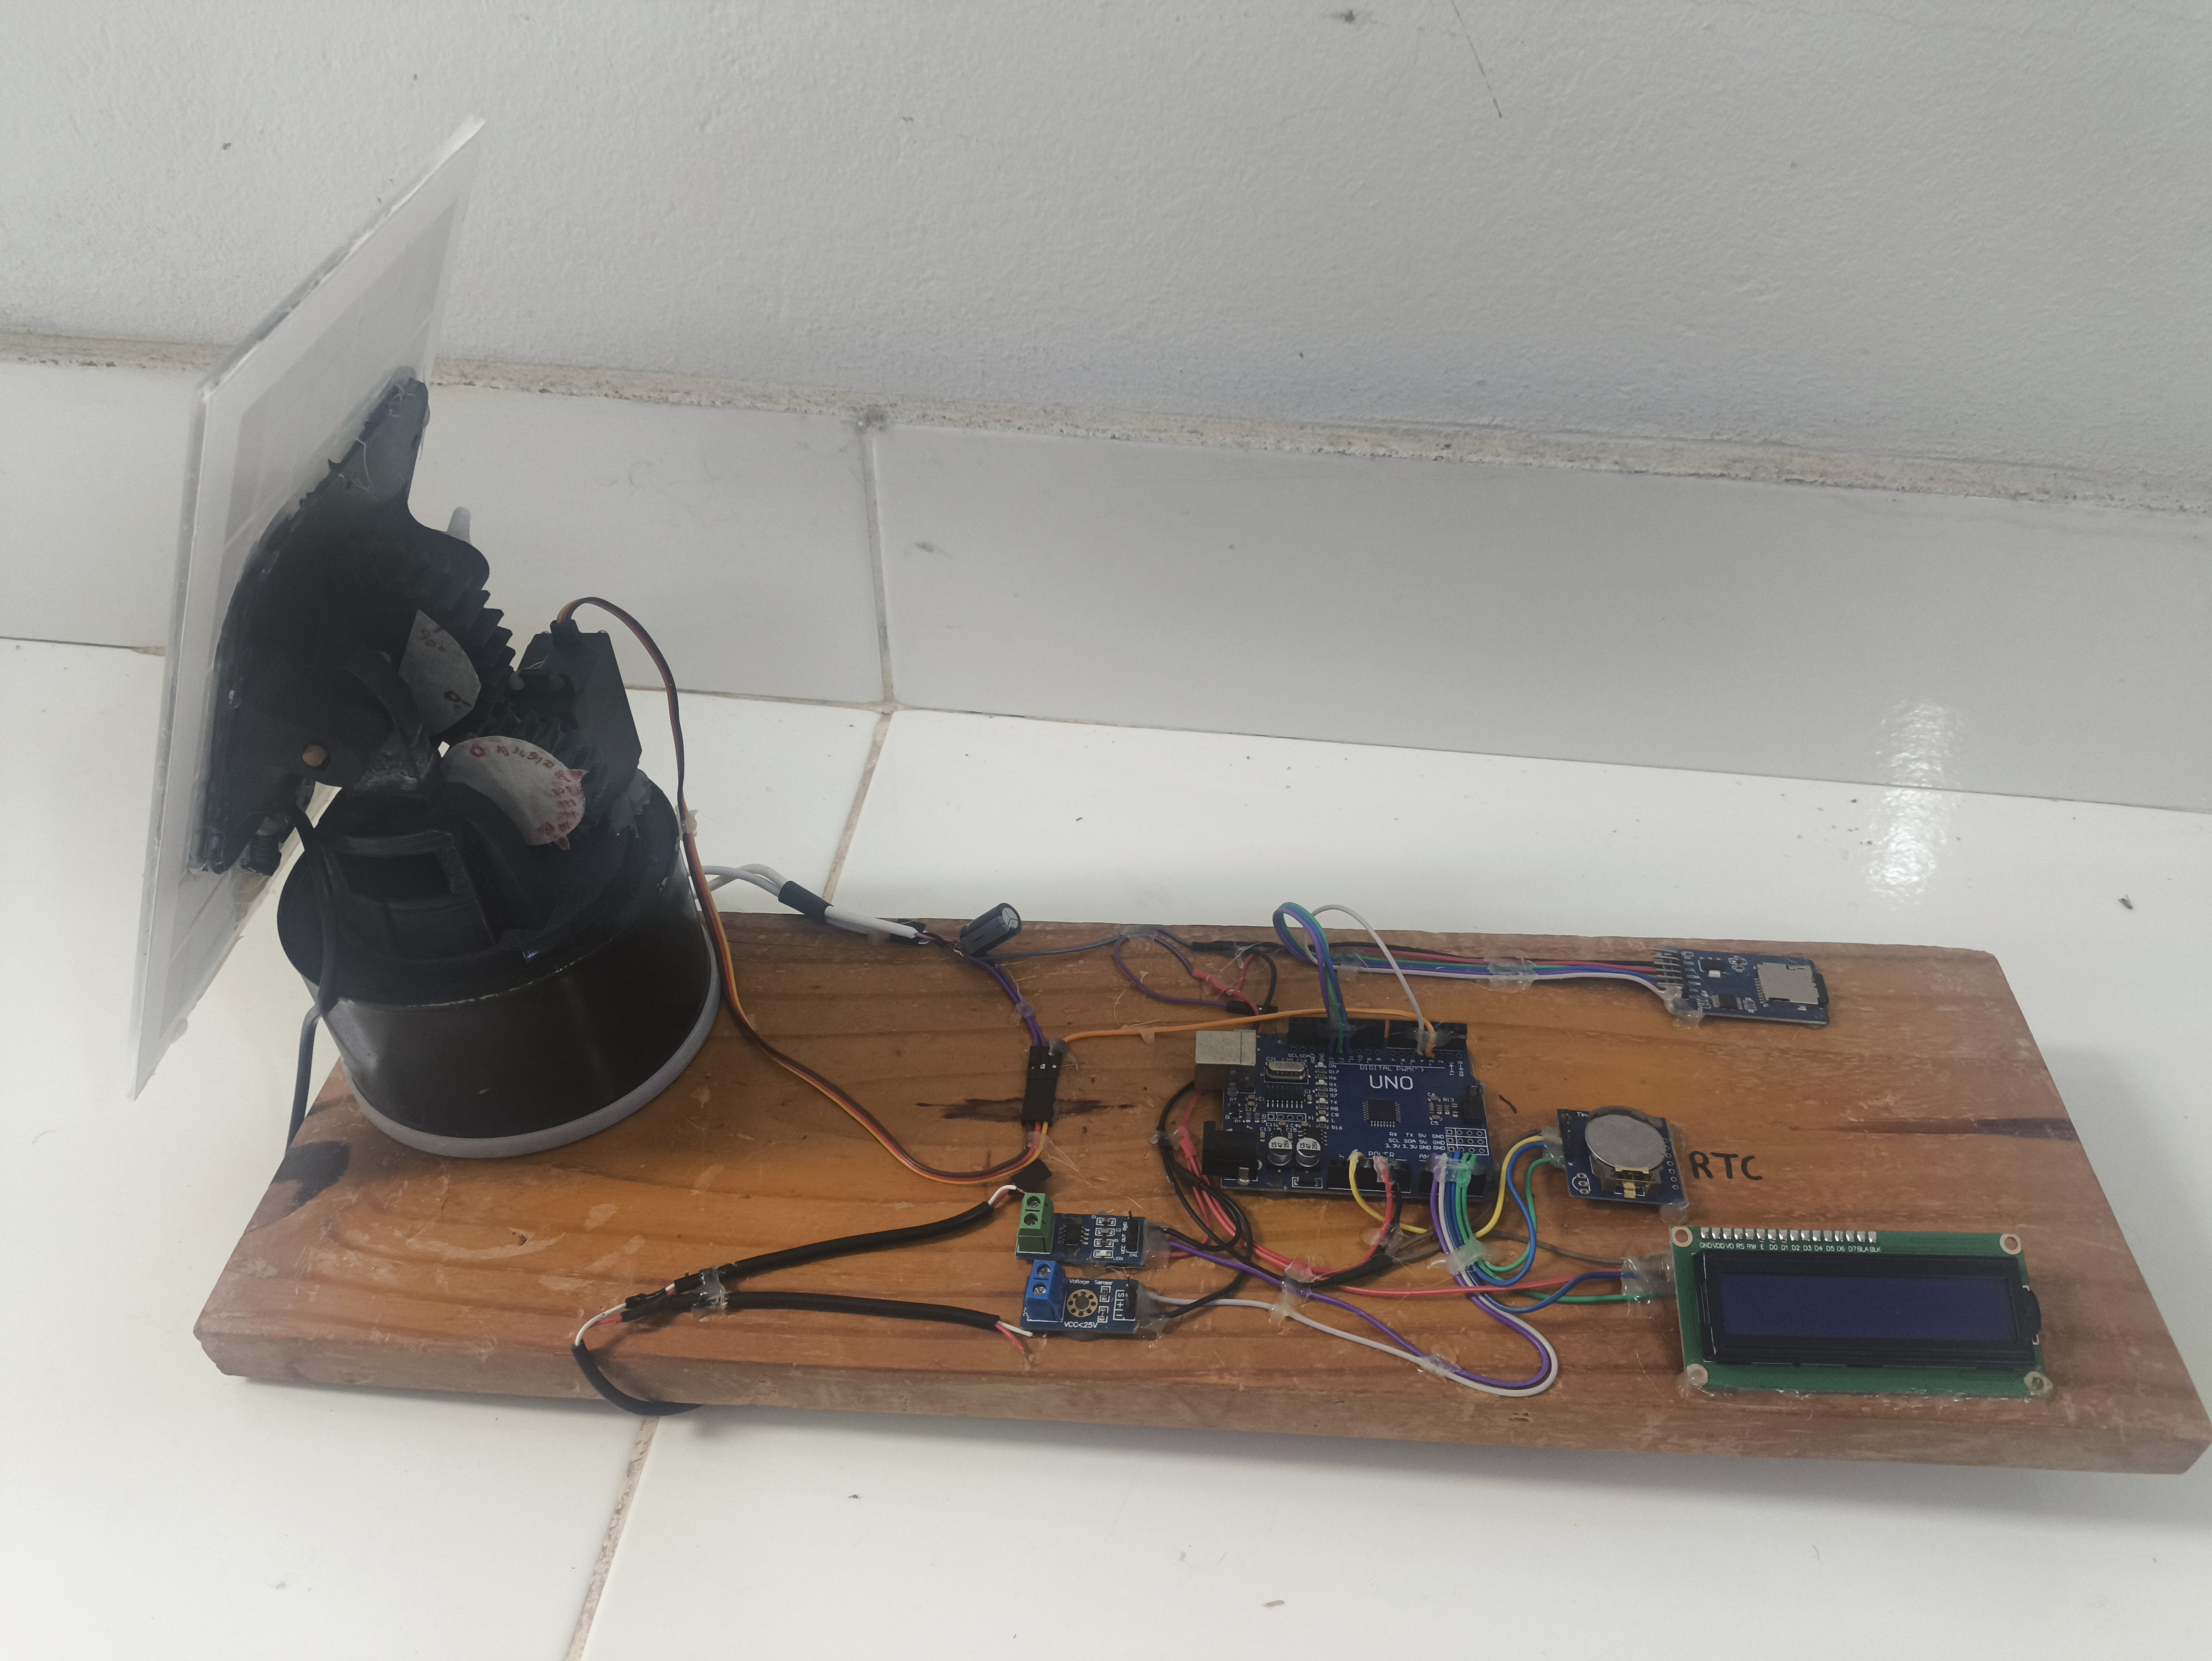
\includegraphics[width=0.6\linewidth]{Figuras/prototipo_montado.jpg}
    \caption{Protótipo do sistema automatizado desenvolvido.}
    \label{fig:prototipo_montado}
    \fonte{Autor (2026).}
\end{figure}

Como os ensaios foram realizados em ambiente externo, foi construída uma estrutura de proteção destinada a minimizar a exposição dos componentes eletrônicos à chuva, à umidade, à radiação solar direta, à poeira e a outros agentes externos, preservando a integridade do sistema durante a coleta de dados.

A estrutura de proteção construída é apresentada na Figura~\ref{fig:protecao_prototipo}.

\begin{figure}[H]
    \centering
    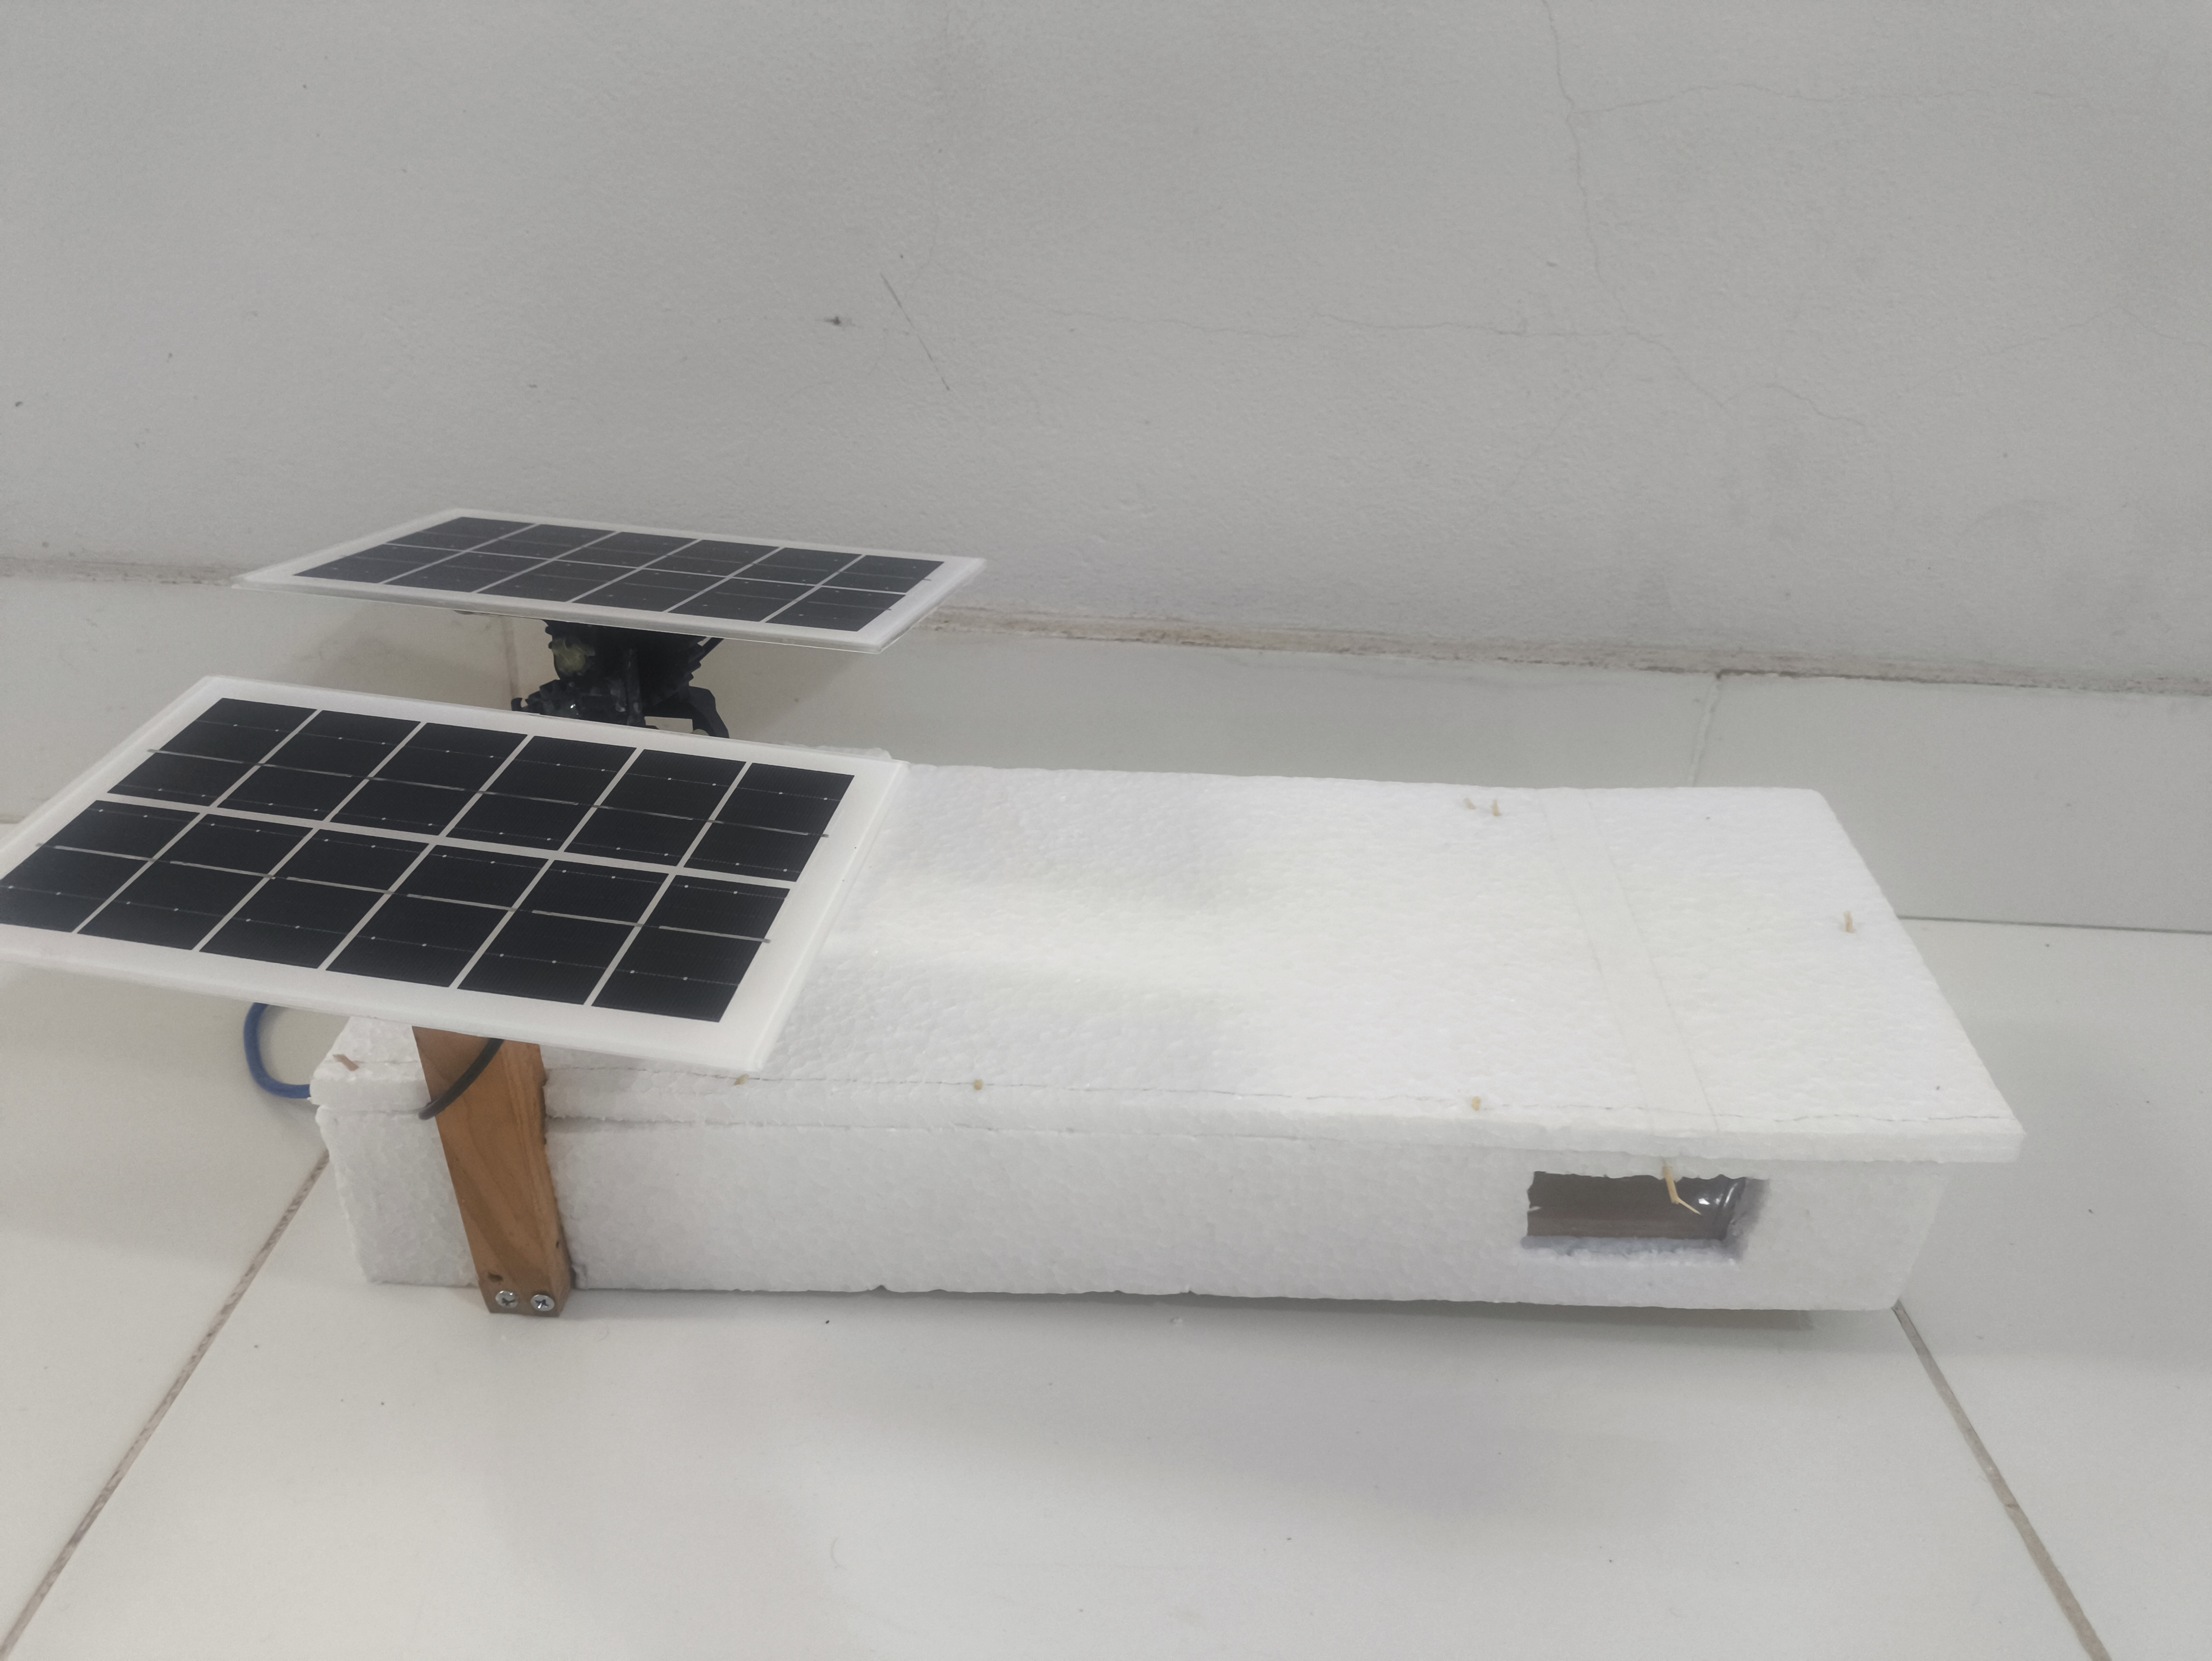
\includegraphics[width=0.7\linewidth]{Figuras/proteçao_prototipo.jpg}
    \caption{Estrutura de proteção do protótipo durante os experimentos.}
    \label{fig:protecao_prototipo}
    \fonte{Autor (2026).}
\end{figure}

A integração entre a estrutura mecânica, o sistema de acionamento e os módulos eletrônicos resultou em um protótipo capaz de realizar automaticamente o posicionamento do painel fotovoltaico, a aquisição das grandezas elétricas e o armazenamento das medições. Esse protótipo constituiu a plataforma experimental utilizada para gerar os dados empregados na validação do modelo computacional e na comparação entre os sistemas automatizado e de painel fixo.

\section{Lógica de Funcionamento do Sistema}

O funcionamento do sistema embarcado foi implementado por meio de um algoritmo de controle responsável por integrar a aquisição de dados, o posicionamento automatizado do painel fotovoltaico, o cálculo das grandezas elétricas e o armazenamento das informações experimentais. O algoritmo foi desenvolvido para operar continuamente durante o período de funcionamento do sistema, permitindo a execução automática das etapas de monitoramento, controle e registro dos dados utilizados na validação do modelo computacional.

A lógica de funcionamento baseia-se na utilização das informações de data e horário fornecidas pelo módulo RTC para determinar o posicionamento do painel fotovoltaico ao longo do dia. Além disso, são realizados pequenos ajustes no posicionamento a partir da potência elétrica medida, com o objetivo de corrigir eventuais diferenças entre a posição teórica e a condição de maior geração de energia.

As subseções seguintes apresentam o fluxograma do algoritmo e descrevem detalhadamente as principais etapas de funcionamento implementadas no sistema embarcado.

\subsection{Fluxograma do Algoritmo}

A lógica de funcionamento do sistema foi implementada no microcontrolador Arduino, responsável por executar as rotinas de inicialização, aquisição de dados, controle do posicionamento do painel fotovoltaico e armazenamento das informações coletadas.

O algoritmo foi desenvolvido de forma sequencial, integrando a leitura do módulo RTC, a determinação do ângulo de posicionamento, o acionamento do servomotor, a aquisição das variáveis elétricas e o registro dos dados em cartão microSD. A Figura~\ref{fig:fluxograma} apresenta o fluxograma simplificado do algoritmo implementado no sistema embarcado.

\begin{figure}[htbp]
\centering
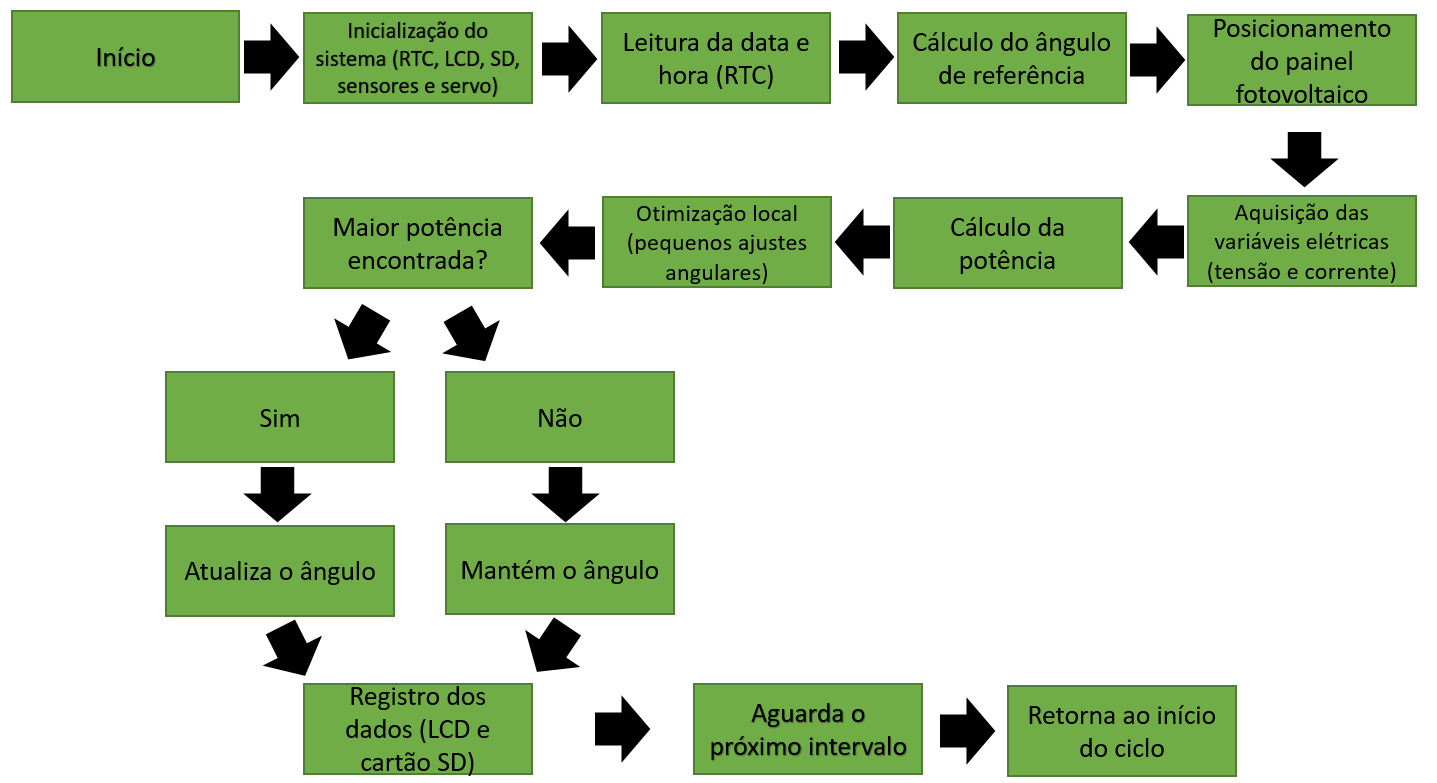
\includegraphics[width=0.90\textwidth]{Figuras/fluxograma_algoritimo.png}
\caption{Fluxograma do algoritmo de controle implementado no sistema automatizado.}
\label{fig:fluxograma}
\fonte{Autor (2026).}
\end{figure}

O algoritmo inicia com a configuração dos módulos de comunicação, dos sensores, do servomotor, do display LCD, do módulo RTC e do cartão microSD. Após essa etapa, entra em um ciclo contínuo de execução durante o período de funcionamento do sistema.

Inicialmente, são obtidas a data e a hora fornecidas pelo módulo RTC. Com base nessas informações, é determinado o ângulo de referência correspondente ao horário atual, utilizado como posição inicial do painel fotovoltaico.

Na sequência, são realizadas as leituras dos sensores de tensão e corrente, permitindo o cálculo da potência elétrica instantânea produzida pelo painel fotovoltaico.

Em seguida, é executada uma rotina de ajuste fino do posicionamento, na qual são realizados pequenos deslocamentos angulares em torno da posição de referência, comparando-se a potência elétrica obtida em cada posição. Ao final dessa etapa, o painel é reposicionado no ângulo que apresentou a maior potência medida.

Após a definição da posição final, os valores de tensão, corrente, potência, ângulo, data e horário são apresentados no display LCD e registrados automaticamente no cartão microSD. Em seguida, o algoritmo reinicia o ciclo de operação, repetindo essa sequência durante todo o período de funcionamento do sistema.

\subsection{Controle do Servo Motor}

O posicionamento do painel fotovoltaico é realizado por um servomotor MG996R, acionado pelo microcontrolador Arduino Uno por meio de sinais PWM (\textit{Pulse Width Modulation}). Nessa técnica, a largura do pulso determina a posição angular do eixo do servomotor, permitindo controlar a orientação do painel ao longo do dia.

A estratégia de controle desenvolvida neste trabalho combina um modelo temporal com uma etapa de ajuste baseada na potência elétrica gerada pelo painel fotovoltaico. Inicialmente, o módulo RTC DS1307 fornece ao microcontrolador as informações de data e horário. A partir desses dados, é calculado o ângulo de referência do painel por meio de uma interpolação linear entre os horários de início e término da operação do sistema, conforme a Equação~\ref{eq:angulo}.

\begin{equation}
\theta=\theta_i+\left(\frac{t-t_i}{t_f-t_i}\right)(\theta_f-\theta_i)
\label{eq:angulo}
\end{equation}

em que $\theta$ representa o ângulo de referência do painel, $\theta_i$ e $\theta_f$ correspondem aos ângulos inicial e final do sistema, respectivamente, enquanto $t$ representa o horário atual fornecido pelo RTC, sendo $t_i$ e $t_f$ os horários de início e término da operação.

Após posicionar o painel no ângulo de referência, o algoritmo executa, a cada 10 minutos, uma rotina de ajuste fino do posicionamento. Esse intervalo foi adotado por representar um compromisso entre a necessidade de acompanhar o deslocamento aparente do Sol e a redução do número de acionamentos do servomotor, minimizando o desgaste mecânico e o consumo de energia do sistema.

Durante essa etapa, o servomotor realiza pequenos deslocamentos angulares em torno da posição de referência, efetuando medições de tensão e corrente em cada posição avaliada. A potência elétrica instantânea é determinada por meio da Equação~\ref{eq:potencia}.

\begin{equation}
P = V \cdot I
\label{eq:potencia}
\end{equation}

em que $P$ representa a potência elétrica gerada pelo painel fotovoltaico (W), $V$ corresponde à tensão elétrica medida nos terminais do painel (V) e $I$ representa a corrente elétrica fornecida pelo módulo fotovoltaico (A).

Embora os métodos de rastreamento do ponto de máxima potência (\textit{Maximum Power Point Tracking} -- MPPT) tenham como objetivo maximizar a potência extraída dos módulos fotovoltaicos por meio do ajuste contínuo do ponto de operação elétrico do sistema \cite{esram2007}, neste trabalho não foi implementado um algoritmo MPPT. A potência elétrica medida pelos sensores foi utilizada apenas como variável de referência para realizar pequenos ajustes na orientação mecânica do painel fotovoltaico, buscando identificar a posição que proporciona a maior geração de energia.

Essa estratégia permite compensar pequenas diferenças entre a posição teórica do Sol e as condições reais de operação, como variações de irradiância, nebulosidade, desalinhamentos mecânicos e pequenas imprecisões construtivas. Ao término da rotina de ajuste, o painel é reposicionado automaticamente no ângulo correspondente ao maior valor de potência medido.

Ao final de cada ciclo de controle, o microcontrolador registra automaticamente no cartão microSD as informações de data, horário, tensão, corrente, potência e ângulo de posicionamento do painel. Simultaneamente, essas variáveis são apresentadas em tempo real no display LCD, permitindo o acompanhamento contínuo da operação do sistema durante os ensaios experimentais.

A Figura~\ref{fig:esquema} apresenta a integração entre o microcontrolador, o servomotor e os demais dispositivos utilizados no sistema de controle.

\begin{figure}[H]
    \centering
    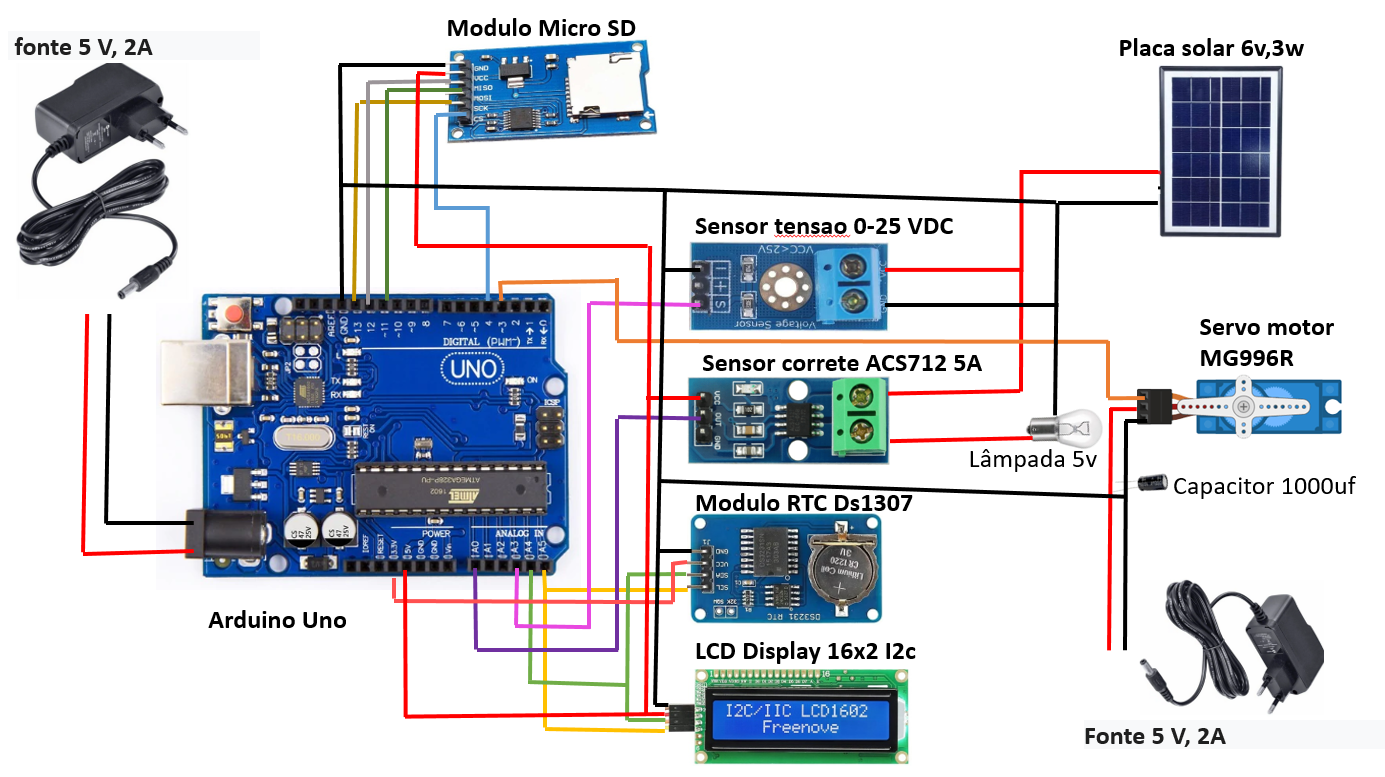
\includegraphics[width=0.9\textwidth]{Figuras/esquema.png}
    \caption{Integração entre o microcontrolador, o servomotor e os demais módulos do sistema.}
    \label{fig:esquema}
    \fonte{Autor (2026).}
\end{figure}

\subsection{Aquisição dos Dados}

A aquisição dos dados foi realizada continuamente durante o funcionamento do sistema embarcado, sendo coordenada pelo microcontrolador Arduino Uno. Após cada ciclo de posicionamento do painel fotovoltaico, o sistema realiza a leitura das grandezas elétricas por meio dos sensores de tensão e corrente, processa as informações obtidas e calcula a potência elétrica correspondente.

As leituras são realizadas pelas entradas analógicas do microcontrolador, que converte os sinais provenientes dos sensores em valores digitais por meio do conversor analógico-digital (ADC) de 10 bits. Em seguida, esses valores são convertidos para suas respectivas unidades físicas utilizando os fatores de calibração adotados para cada sensor.

A potência elétrica instantânea gerada pelo painel fotovoltaico é calculada a partir das medições de tensão e corrente, conforme a Equação~\ref{eq:potencia}.

Após o processamento das medições, o sistema associa automaticamente cada registro às informações de data e horário fornecidas pelo módulo RTC DS1307. Os dados são então armazenados automaticamente, em intervalos de um minuto, em um cartão microSD no formato texto (.txt), formando uma série temporal das variáveis monitoradas.

Cada registro contém as seguintes informações:

\begin{itemize}
    \item data da medição;
    \item horário da aquisição;
    \item tensão elétrica (V);
    \item corrente elétrica (A);
    \item potência elétrica (W);
    \item ângulo de posicionamento do painel (°).
\end{itemize}

Além do armazenamento permanente no cartão microSD, as principais variáveis monitoradas são apresentadas em tempo real no display LCD, permitindo acompanhar o funcionamento do sistema durante os ensaios experimentais. Os registros completos obtidos durante os experimentos encontram-se apresentados no Apêndice~\ref{ap:apendiceC}.

A frequência de aquisição de um minuto foi definida por representar adequadamente a variação das grandezas elétricas ao longo do período de operação, possibilitando a obtenção de uma base de dados representativa sem gerar um volume excessivo de registros. Os dados coletados foram posteriormente utilizados na análise do desempenho do sistema automatizado e na validação do modelo computacional desenvolvido no ambiente MATLAB/Simulink.

\section{Modelagem e Simulação Computacional}
\label{sec:modelagem_simulacao}

A modelagem computacional constituiu uma etapa fundamental deste trabalho, sendo utilizada para representar o comportamento do sistema fotovoltaico automatizado e possibilitar sua comparação com os resultados obtidos experimentalmente. Dessa forma, o modelo desenvolvido serviu como base para a validação da capacidade da simulação em representar o comportamento observado no protótipo físico.

O modelo computacional foi implementado no ambiente MATLAB/Simulink a partir do trabalho disponibilizado por Nagi (\citeyear{nagi2023}), sendo realizadas adaptações para representar as características do sistema desenvolvido nesta pesquisa. A partir desse modelo, foram simulados um sistema fotovoltaico automatizado e um sistema com painel fixo, permitindo comparar seu desempenho energético com os resultados experimentais obtidos durante os ensaios realizados.

As subseções seguintes apresentam a modelagem matemática adotada, o desenvolvimento do modelo computacional no ambiente MATLAB/Simulink e o procedimento utilizado para sua validação por meio da comparação entre os resultados simulados e os dados experimentais obtidos com o protótipo físico.

A trajetória aparente do Sol foi representada por uma função senoidal, utilizada para reproduzir qualitativamente a variação diária da incidência da radiação solar sobre o painel fotovoltaico. Essa aproximação permite representar o comportamento do sistema ao longo do período de simulação sem recorrer a modelos astronômicos mais complexos.

\begin{equation}
S(t)=\sin\left(\frac{\pi t}{12}\right)
\label{eq:trajetoria}
\end{equation}

em que S(t) representa a posição relativa do Sol ao longo do dia e t corresponde ao tempo de simulação, expresso em horas.

Para representar a irradiância incidente sobre o painel, o modelo considera uma componente direta e uma componente difusa. Na implementação realizada foram adotados valores constantes de 900 W/m² para a irradiância direta máxima e 100 W/m² para a irradiância difusa, totalizando aproximadamente 1000 W/m² nas condições de máxima incidência, valor compatível com as Condições Padrão de Teste (STC).

No sistema automatizado, a potência simulada é considerada proporcional à irradiância incidente sobre o painel. Para o sistema com painel fixo, foi introduzido um fator angular que reduz a parcela da irradiância direta recebida pelo módulo em função do desalinhamento entre o painel e a posição aparente do Sol. Dessa forma, o sistema fixo apresenta menor geração de potência durante parte do período de operação quando comparado ao sistema automatizado.

A energia produzida por cada configuração foi obtida por meio da integração da potência ao longo do tempo, conforme a Equação~\ref{eq:energia}.

\begin{equation}
E=\int P(t),dt
\label{eq:energia}
\end{equation}

em que E representa a energia acumulada e P(t) corresponde à potência instantânea produzida pelo sistema.

O ganho percentual do sistema automatizado em relação ao sistema com painel fixo foi determinado pela Equação~\ref{eq:ganho}.

\begin{equation}
G(%)=
\frac{E_{aut}-E_{fixo}}
{E_{fixo}}
\times100
\label{eq:ganho}
\end{equation}

em que $E_{aut}$ representa a energia produzida pelo sistema automatizado e $E_{fixo}$ representa a energia produzida pelo sistema com painel fixo.

No protótipo físico, a potência elétrica foi determinada experimentalmente a partir das medições de tensão e corrente realizadas pelos sensores instalados no sistema, utilizando a Equação~\ref{eq:potencia}.

\begin{equation}
P=V\cdot I
\label{eq:potencia}
\end{equation}

em que V representa a tensão elétrica (V) e I corresponde à corrente elétrica (A).

As relações apresentadas constituem a base matemática utilizada na simulação e permitiram comparar o comportamento energético obtido no modelo computacional com os resultados experimentais obtidos pelo protótipo físico.


\subsection{Desenvolvimento do Modelo Computacional no MATLAB/Simulink}
\label{subsec:desenvolvimento_modelo}

O modelo computacional foi implementado no ambiente MATLAB utilizando a ferramenta Simulink, empregada na modelagem e simulação de sistemas dinâmicos por meio de diagramas de blocos. Como base para o desenvolvimento, foi utilizado o modelo disponibilizado por Nagi (\citeyear{nagi2023}), no qual foram realizadas adaptações para representar as características do sistema automatizado desenvolvido neste trabalho.

A Figura~\ref{fig:simulink_modelo} apresenta o diagrama de blocos do modelo computacional implementado.

\begin{figure}[H]
\centering
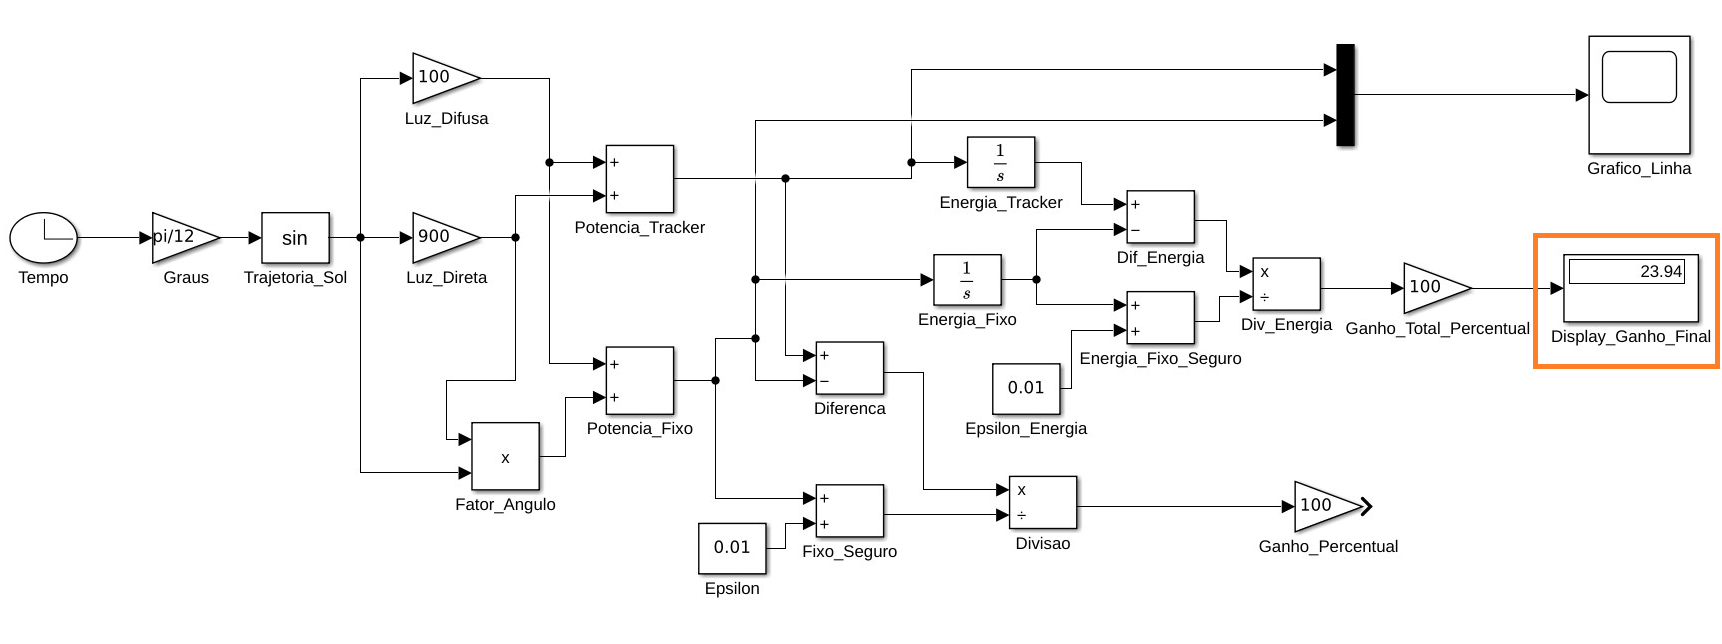
\includegraphics[width=\textwidth]{Figuras/MS.png}
\caption{Modelo computacional desenvolvido no ambiente MATLAB/Simulink.}
\label{fig:simulink_modelo}
\fonte{Autor (2026).}
\end{figure}

O funcionamento do modelo inicia-se com o bloco \textit{Clock}, responsável por fornecer o tempo da simulação. Em seguida, esse sinal é convertido em radianos por um bloco de ganho e aplicado a uma função seno, utilizada para representar de forma simplificada a trajetória aparente do Sol ao longo do dia. A partir desse sinal são geradas as componentes de irradiância empregadas no cálculo da potência produzida pelo sistema automatizado e pelo sistema com painel fixo. Posteriormente, o modelo determina a energia acumulada e o ganho percentual entre as duas configurações, permitindo a comparação dos resultados simulados com os dados obtidos experimentalmente.

De acordo com o Centro de Referência para Energia Solar e Eólica Sérgio de Salvo Brito (CRESESB), a irradiância solar extraterrestre apresenta valor médio próximo de 1361 W/m², conhecido como constante solar \cite{cresesb}. Entretanto, devido aos fenômenos de absorção, reflexão e espalhamento da radiação na atmosfera terrestre, a irradiância disponível na superfície é reduzida. Em condições atmosféricas favoráveis e céu limpo, a irradiância incidente pode atingir aproximadamente 1000 W/m², valor adotado internacionalmente como Condição Padrão de Teste (\textit{Standard Test Conditions} -- STC) para caracterização de módulos fotovoltaicos \cite{solarscope}.

Conforme descrito na Seção~\ref{sec:modelagem_simulacao}, o modelo considera uma irradiância direta máxima de 900 W/m² e uma componente difusa de 100 W/m², totalizando aproximadamente 1000 W/m² nas Condições Padrão de Teste (STC). O período de simulação foi definido em 12 horas, representando o intervalo diário de disponibilidade de radiação solar.

Para o sistema automatizado, considerou-se que o painel permanece continuamente orientado na direção de maior incidência da radiação solar, recebendo integralmente as componentes direta e difusa da irradiância.

No sistema com painel fixo, a componente direta da irradiância foi ponderada por um fator angular, representando as perdas decorrentes do desalinhamento entre o painel e a posição aparente do Sol. Dessa forma, o modelo representa a redução da potência produzida ao longo do dia em função da variação do ângulo de incidência da radiação solar.

As potências instantâneas produzidas pelos dois sistemas foram integradas ao longo do tempo para determinação da energia acumulada durante o período de simulação. Em seguida, foi calculado o ganho percentual do sistema automatizado em relação ao sistema com painel fixo, permitindo comparar diretamente o desempenho energético das duas configurações.

Ao término da simulação, o modelo fornece as curvas de potência dos sistemas automatizado e de painel fixo, além da energia acumulada e do ganho percentual calculado entre as duas configurações. Esses dados foram posteriormente utilizados na comparação com os resultados obtidos experimentalmente.

O código-fonte desenvolvido para a implementação do modelo computacional no MATLAB/Simulink encontra-se disponibilizado no Apêndice~\ref{ap:github}, permitindo a reprodução da simulação apresentada neste trabalho.

\subsection{Validação do Modelo Computacional}
\label{subsec:validacao_modelo}

Após o desenvolvimento do modelo computacional, foi realizada sua validação por meio da comparação entre os resultados obtidos na simulação e os dados experimentais coletados pelo protótipo físico desenvolvido neste trabalho.

Para garantir a comparabilidade entre os resultados, a simulação e os ensaios experimentais foram conduzidos considerando o mesmo período diário de operação e configurações equivalentes para os sistemas fotovoltaicos automatizado e com painel fixo.

A validação consistiu na comparação das curvas das grandezas elétricas obtidas na simulação com aquelas medidas experimentalmente, incluindo tensão elétrica, potência e ganho percentual em relação ao sistema de painel fixo. Além da análise gráfica, foram avaliadas as diferenças entre os valores simulados e experimentais, verificando a capacidade do modelo computacional em representar o comportamento observado no sistema físico.

Os resultados dessa comparação são apresentados e discutidos no Capítulo~\ref{cap5_resultados}, onde é analisado o grau de concordância entre a simulação computacional e o protótipo experimental, permitindo avaliar a representatividade do modelo desenvolvido.

\section{Protocolo Experimental}

Após o desenvolvimento do protótipo e da implementação do modelo computacional, foram realizados ensaios experimentais com o objetivo de comparar o desempenho do sistema fotovoltaico automatizado com o de um sistema de painel fixo. Para garantir a comparabilidade entre os sistemas, ambos foram submetidos às mesmas condições ambientais durante todo o período de coleta de dados, permitindo avaliar a influência do posicionamento automatizado sobre a geração de energia elétrica.

As subseções seguintes descrevem o local de instalação do protótipo, os procedimentos adotados durante os ensaios experimentais e os métodos empregados no tratamento dos dados coletados, os quais foram posteriormente utilizados na comparação com os resultados obtidos pelo modelo computacional.


\subsection{Local de Instalação}

Os ensaios experimentais foram realizados na cidade de Salinas, localizada no norte do estado de Minas Gerais. O protótipo foi instalado em uma área aberta, livre de obstáculos que pudessem provocar sombreamento ao longo do período de coleta de dados, garantindo que os dois sistemas fossem submetidos às mesmas condições de irradiância durante os experimentos.

As coordenadas geográficas aproximadas do local de instalação são:

\begin{itemize}
    \item Latitude: $16,17^\circ$ S;
    \item Longitude: $42,29^\circ$ O.
\end{itemize}

O protótipo foi instalado sobre uma superfície nivelada, proporcionando estabilidade mecânica durante todo o período experimental.

O sistema automatizado realizava o posicionamento do painel fotovoltaico em um único eixo (Leste--Oeste). Diariamente, o painel iniciava sua operação às 06h00 voltado para leste e era movimentado automaticamente em direção ao oeste até as 18h00, acompanhando o deslocamento aparente do Sol.

Para fins de comparação, foi utilizado um segundo painel fotovoltaico com as mesmas especificações, mantido em posição fixa durante todo o período experimental. Esse painel permaneceu instalado horizontalmente ($0^\circ$ em relação ao plano horizontal), sem qualquer ajuste de orientação ou posicionamento, permitindo comparar diretamente o desempenho de um sistema estático com o sistema de posicionamento automatizado desenvolvido neste trabalho.

A configuração horizontal foi adotada para ambos os painéis no instante inicial da montagem, de modo que a principal diferença entre os sistemas estivesse relacionada exclusivamente ao posicionamento automatizado do painel ao longo do dia, eliminando a influência de diferentes ângulos de instalação na comparação dos resultados.

\subsection{Procedimentos Experimentais}

Os ensaios experimentais foram realizados entre os dias 23 e 26 de maio de 2026, período selecionado em função das condições climáticas favoráveis, priorizando dias sem ocorrência de precipitação. Como o protótipo permaneceu instalado em ambiente externo durante toda a campanha experimental, essa condição contribuiu para reduzir interferências decorrentes das condições meteorológicas.

Durante os ensaios, o sistema automatizado e o sistema de painel fixo operaram simultaneamente, permanecendo submetidos às mesmas condições de irradiância ao longo de todo o período de coleta de dados. Essa configuração permitiu comparar diretamente o desempenho das duas configurações, minimizando a influência das variações ambientais sobre os resultados experimentais.

A coleta de dados foi realizada diariamente entre 06h00 e 18h00, intervalo correspondente ao período diário de operação do sistema. No início de cada dia, o painel do sistema automatizado era posicionado na direção leste e, ao longo do período de funcionamento, seu ângulo era ajustado automaticamente de acordo com a estratégia de controle implementada no microcontrolador, finalizando sua movimentação na direção oeste. O painel utilizado como referência permaneceu em posição fixa durante todo o experimento.

As medições de tensão elétrica, corrente elétrica, potência, ângulo de posicionamento, data e horário foram realizadas automaticamente em intervalos de um minuto e registradas em arquivos armazenados no cartão microSD. Esses registros constituíram a base de dados utilizada para a comparação entre o sistema automatizado, o sistema de painel fixo e os resultados obtidos pelo modelo computacional desenvolvido no MATLAB/Simulink.

Ao término de cada dia de coleta, os arquivos gerados foram transferidos para um computador, onde passaram pelas etapas de organização e verificação dos dados. Posteriormente, essas informações foram utilizadas na elaboração dos gráficos, tabelas e análises apresentados no Capítulo de Resultados. Os registros completos obtidos durante os ensaios experimentais encontram-se apresentados no Apêndice~\ref{ap:apendiceC}.

\subsection{Tratamento dos Dados}

Os dados registrados pelos sistemas foram exportados para planilhas eletrônicas, onde passaram pelas etapas de organização, conferência e processamento para obtenção dos resultados apresentados neste trabalho.

Inicialmente, os registros foram verificados para identificar possíveis inconsistências decorrentes do processo de aquisição dos dados. Em seguida, foram calculadas as variáveis de interesse, incluindo a potência instantânea, a energia acumulada ao longo do período de operação e o ganho percentual do sistema automatizado em relação ao sistema com painel fixo.

A potência elétrica instantânea foi calculada a partir das medições de tensão e corrente, conforme a Equação~\ref{eq:potencia}.

O ganho percentual de energia do sistema automatizado em relação ao sistema de painel fixo foi determinado pela Equação~\ref{eq:ganho}.

Os resultados obtidos experimentalmente foram organizados em tabelas e gráficos, possibilitando a comparação entre os dois sistemas. Posteriormente, esses resultados também foram comparados aos valores obtidos pelo modelo computacional desenvolvido no MATLAB/Simulink, por meio da análise dos perfis de potência, da energia acumulada e do ganho percentual de energia. Essa etapa permitiu avaliar a capacidade do modelo computacional em representar o comportamento observado no protótipo físico.

%\chapter{Desenvolvimento do sistema} 
\label{cap4_Desenvolvimento_do_sistema} 
\section{Estrutura Mecânica}

Este capítulo apresenta os aspectos relacionados ao desenvolvimento da estrutura mecânica do sistema automatizado, estabelecendo uma base consistente para a construção, operação e validação do protótipo proposto.

Inicialmente, foi projetada uma estrutura mecânica simplificada, com a finalidade de sustentar adequadamente os componentes do sistema e garantir estabilidade durante a operação. A base estrutural foi confeccionada em madeira, material escolhido em razão de sua facilidade de manuseio, baixo custo e resistência mecânica compatível com aplicações em prototipagem.

Sobre essa base, foi desenvolvido um suporte específico para o acoplamento do painel fotovoltaico, fabricado por meio de impressão 3D. A utilização dessa tecnologia proporcionou maior precisão dimensional, flexibilidade no projeto e facilidade na adaptação dos componentes, possibilitando um ajuste geométrico mais adequado entre o painel e o sistema de acionamento.

No suporte projetado, foi fixado um motor, acoplado a um sistema de engrenagens responsável pela transmissão do movimento rotacional ao painel fotovoltaico. Esse conjunto mecânico permite o ajuste angular controlado do painel ao longo do dia, possibilitando o acompanhamento da trajetória aparente do Sol.

As Figuras~\ref{fig:engrenagem1} e~\ref{fig:engrenagem2} apresentam o suporte e as engrenagens desenvolvidas por meio de impressão 3D, utilizadas no sistema de transmissão mecânica do protótipo.
\begin{figure}[H]
    \centering
    \begin{minipage}{0.45\linewidth}
        \centering
        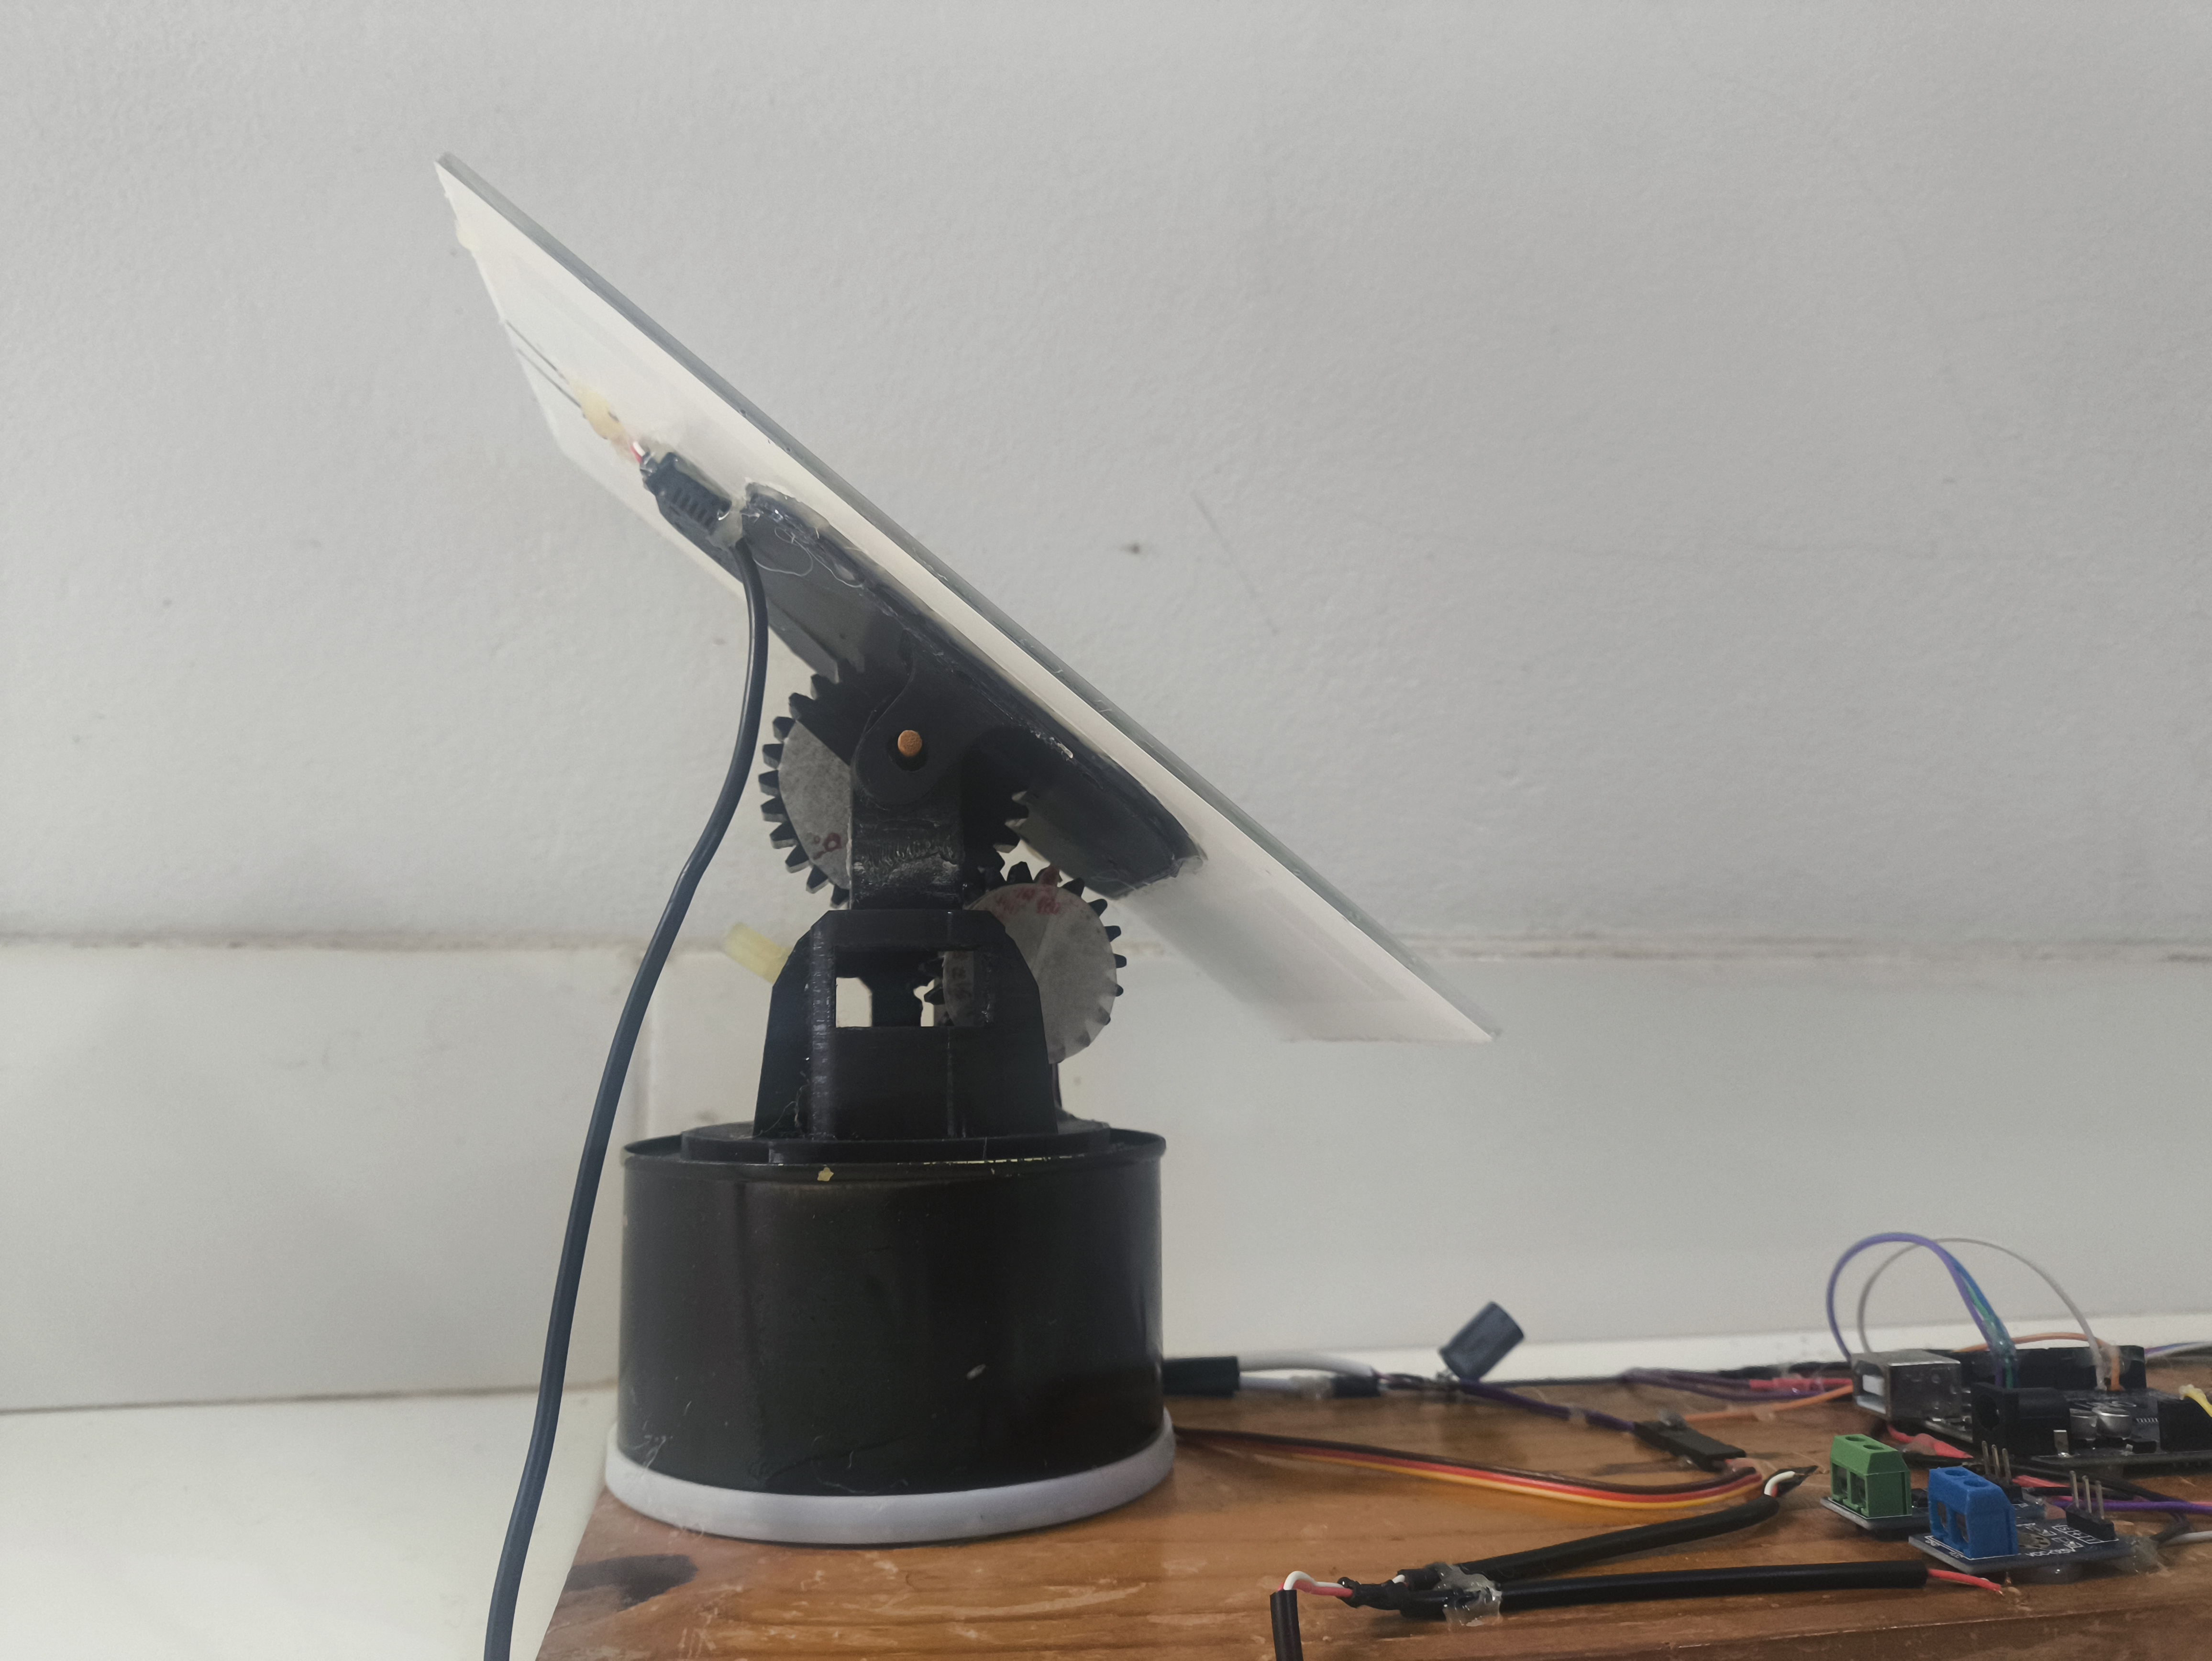
\includegraphics[width=\linewidth]{Figuras/engrenagem1.jpg}
        \caption{Suporte e Engrenagem em 3D}
        \label{fig:engrenagem1}
        \legend{Fonte: Autor (2026).}
    \end{minipage}
    \hfill
    \begin{minipage}{0.45\linewidth}
        \centering
        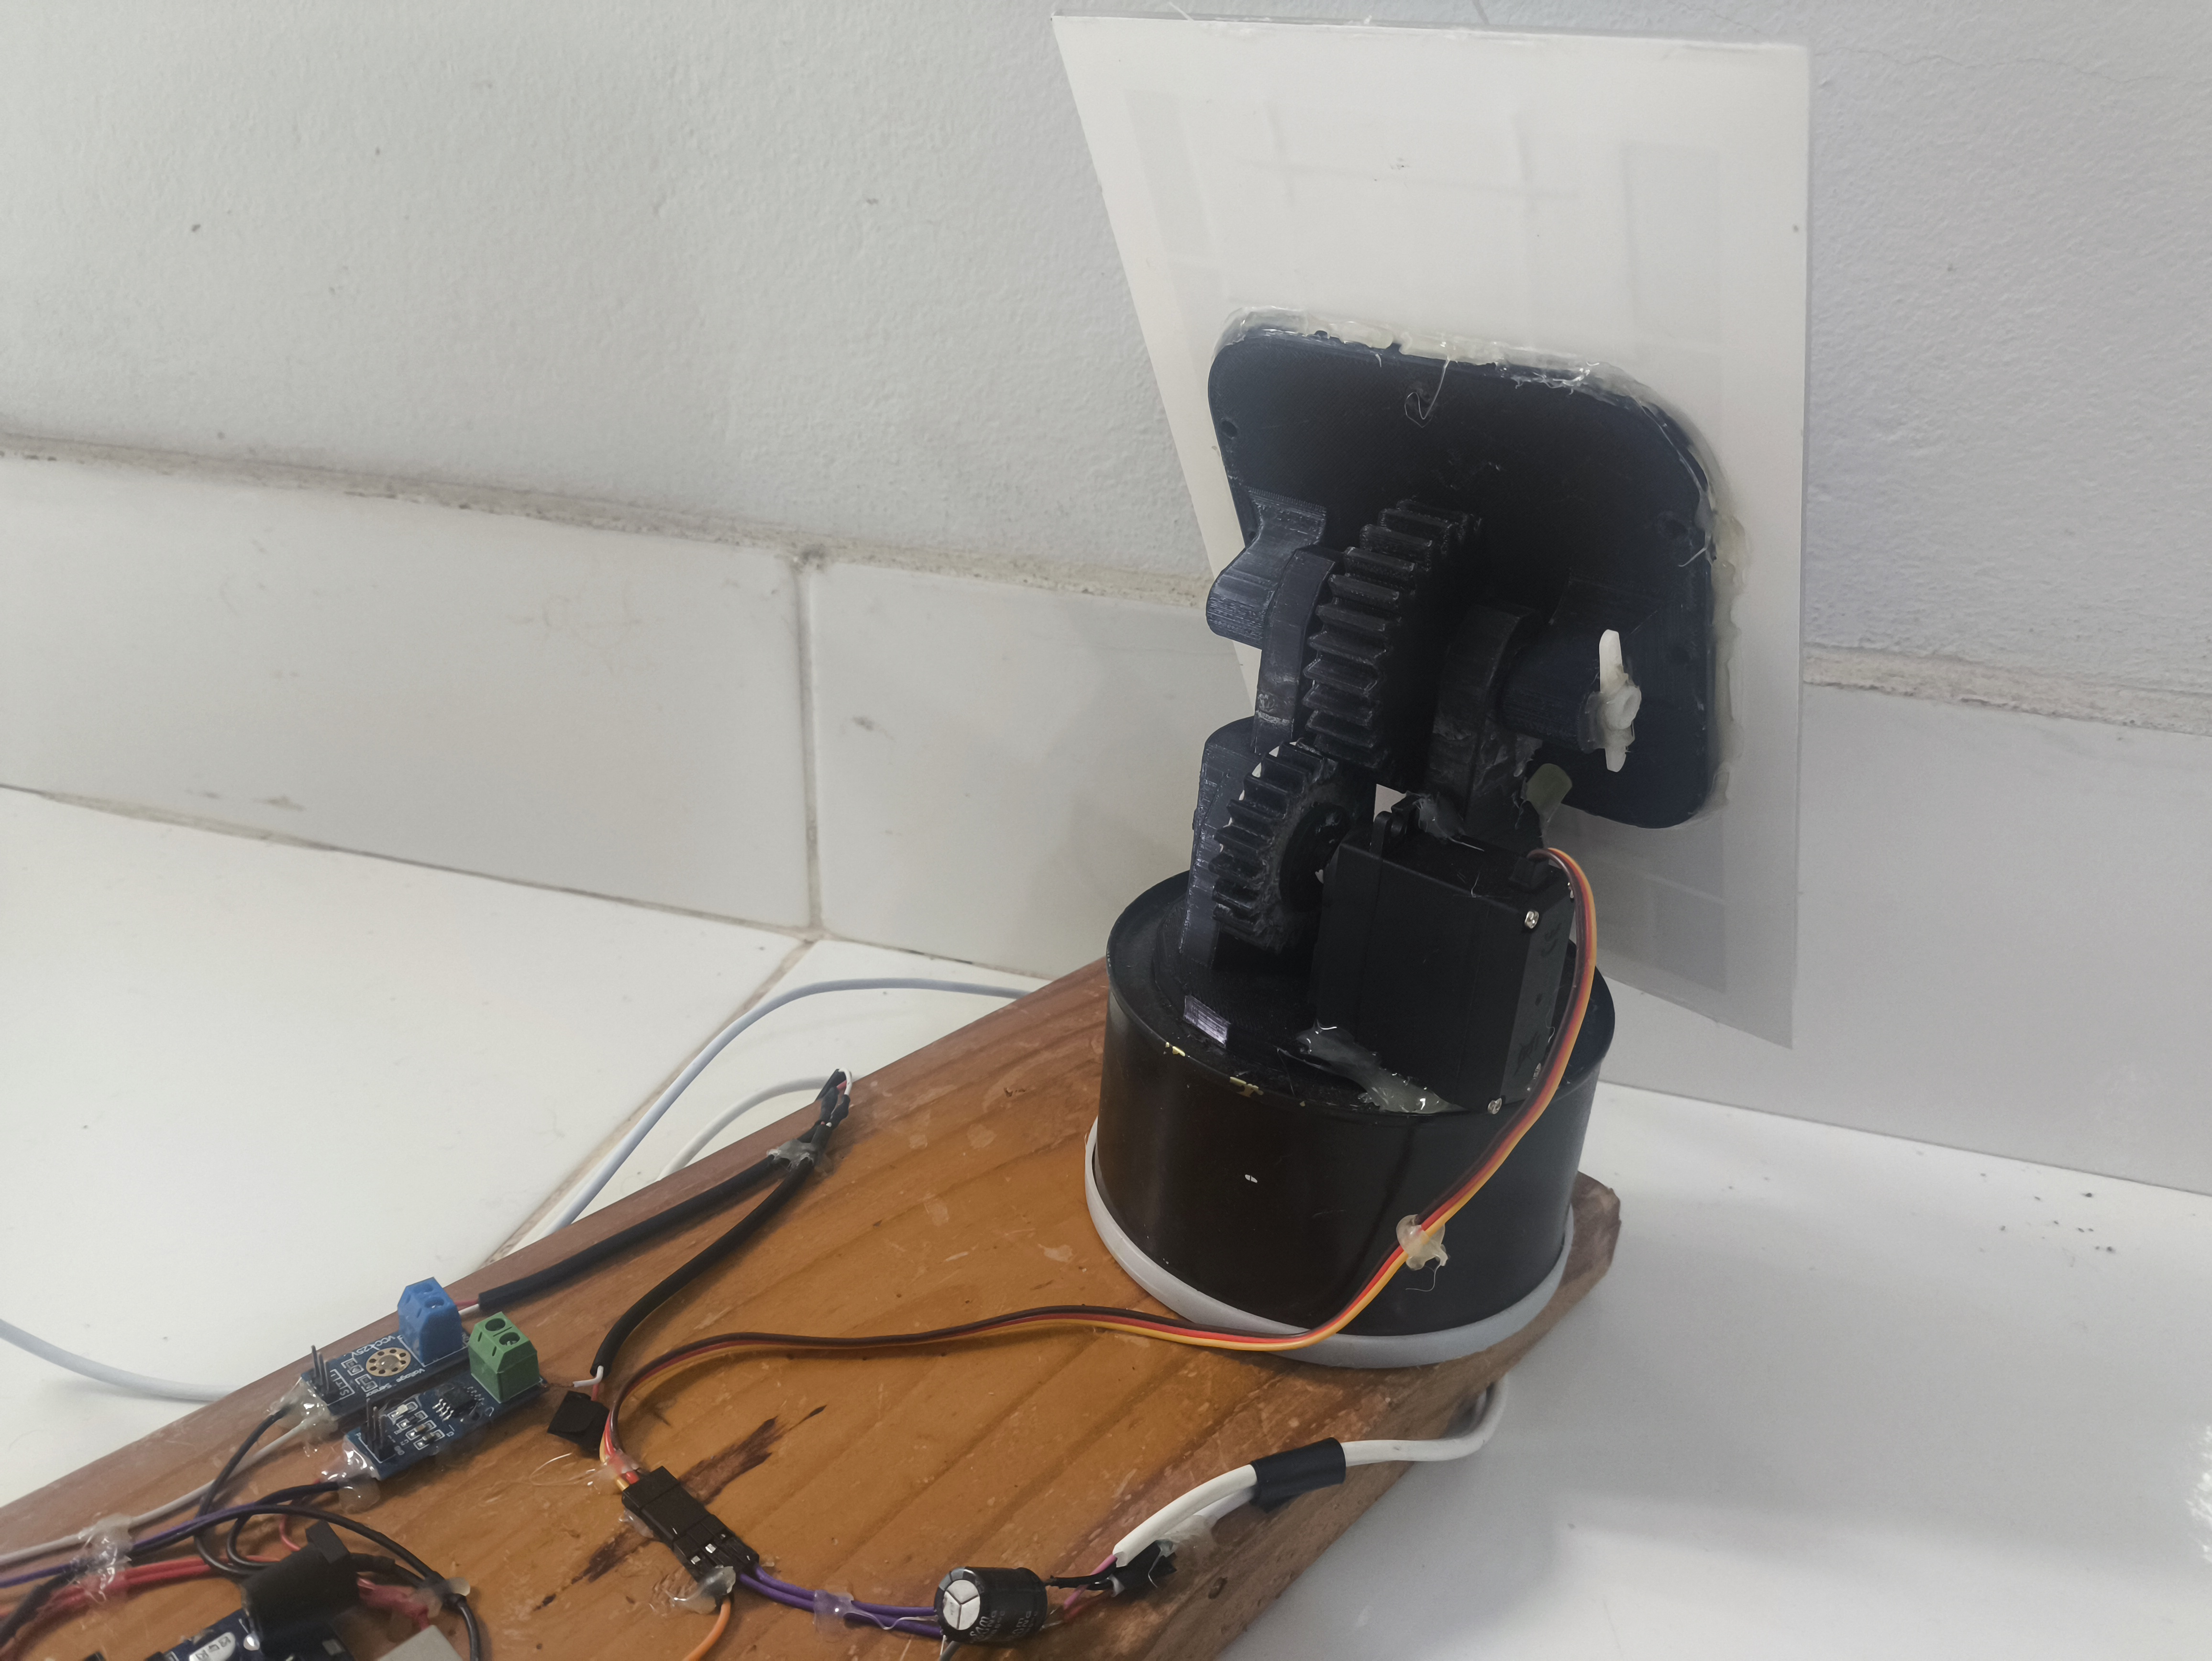
\includegraphics[width=\linewidth]{Figuras/engrenagem2.jpg}
        \caption{Detalhamento da engrenagem}
        \label{fig:engrenagem2}
        \legend{Fonte: Autor (2026).}
    \end{minipage}
\end{figure}

A base também foi utilizada para a fixação dos componentes eletrônicos do sistema de controle, incluindo o microcontrolador, sensores e módulos auxiliares, garantindo organização estrutural, redução de interferências e maior confiabilidade no funcionamento do sistema.

A Figura~\ref{fig:prototipo_montado} apresenta o protótipo do sistema desenvolvido, evidenciando a estrutura mecânica proposta e a disposição dos componentes descritos.
\begin{figure}[H]
    \centering
    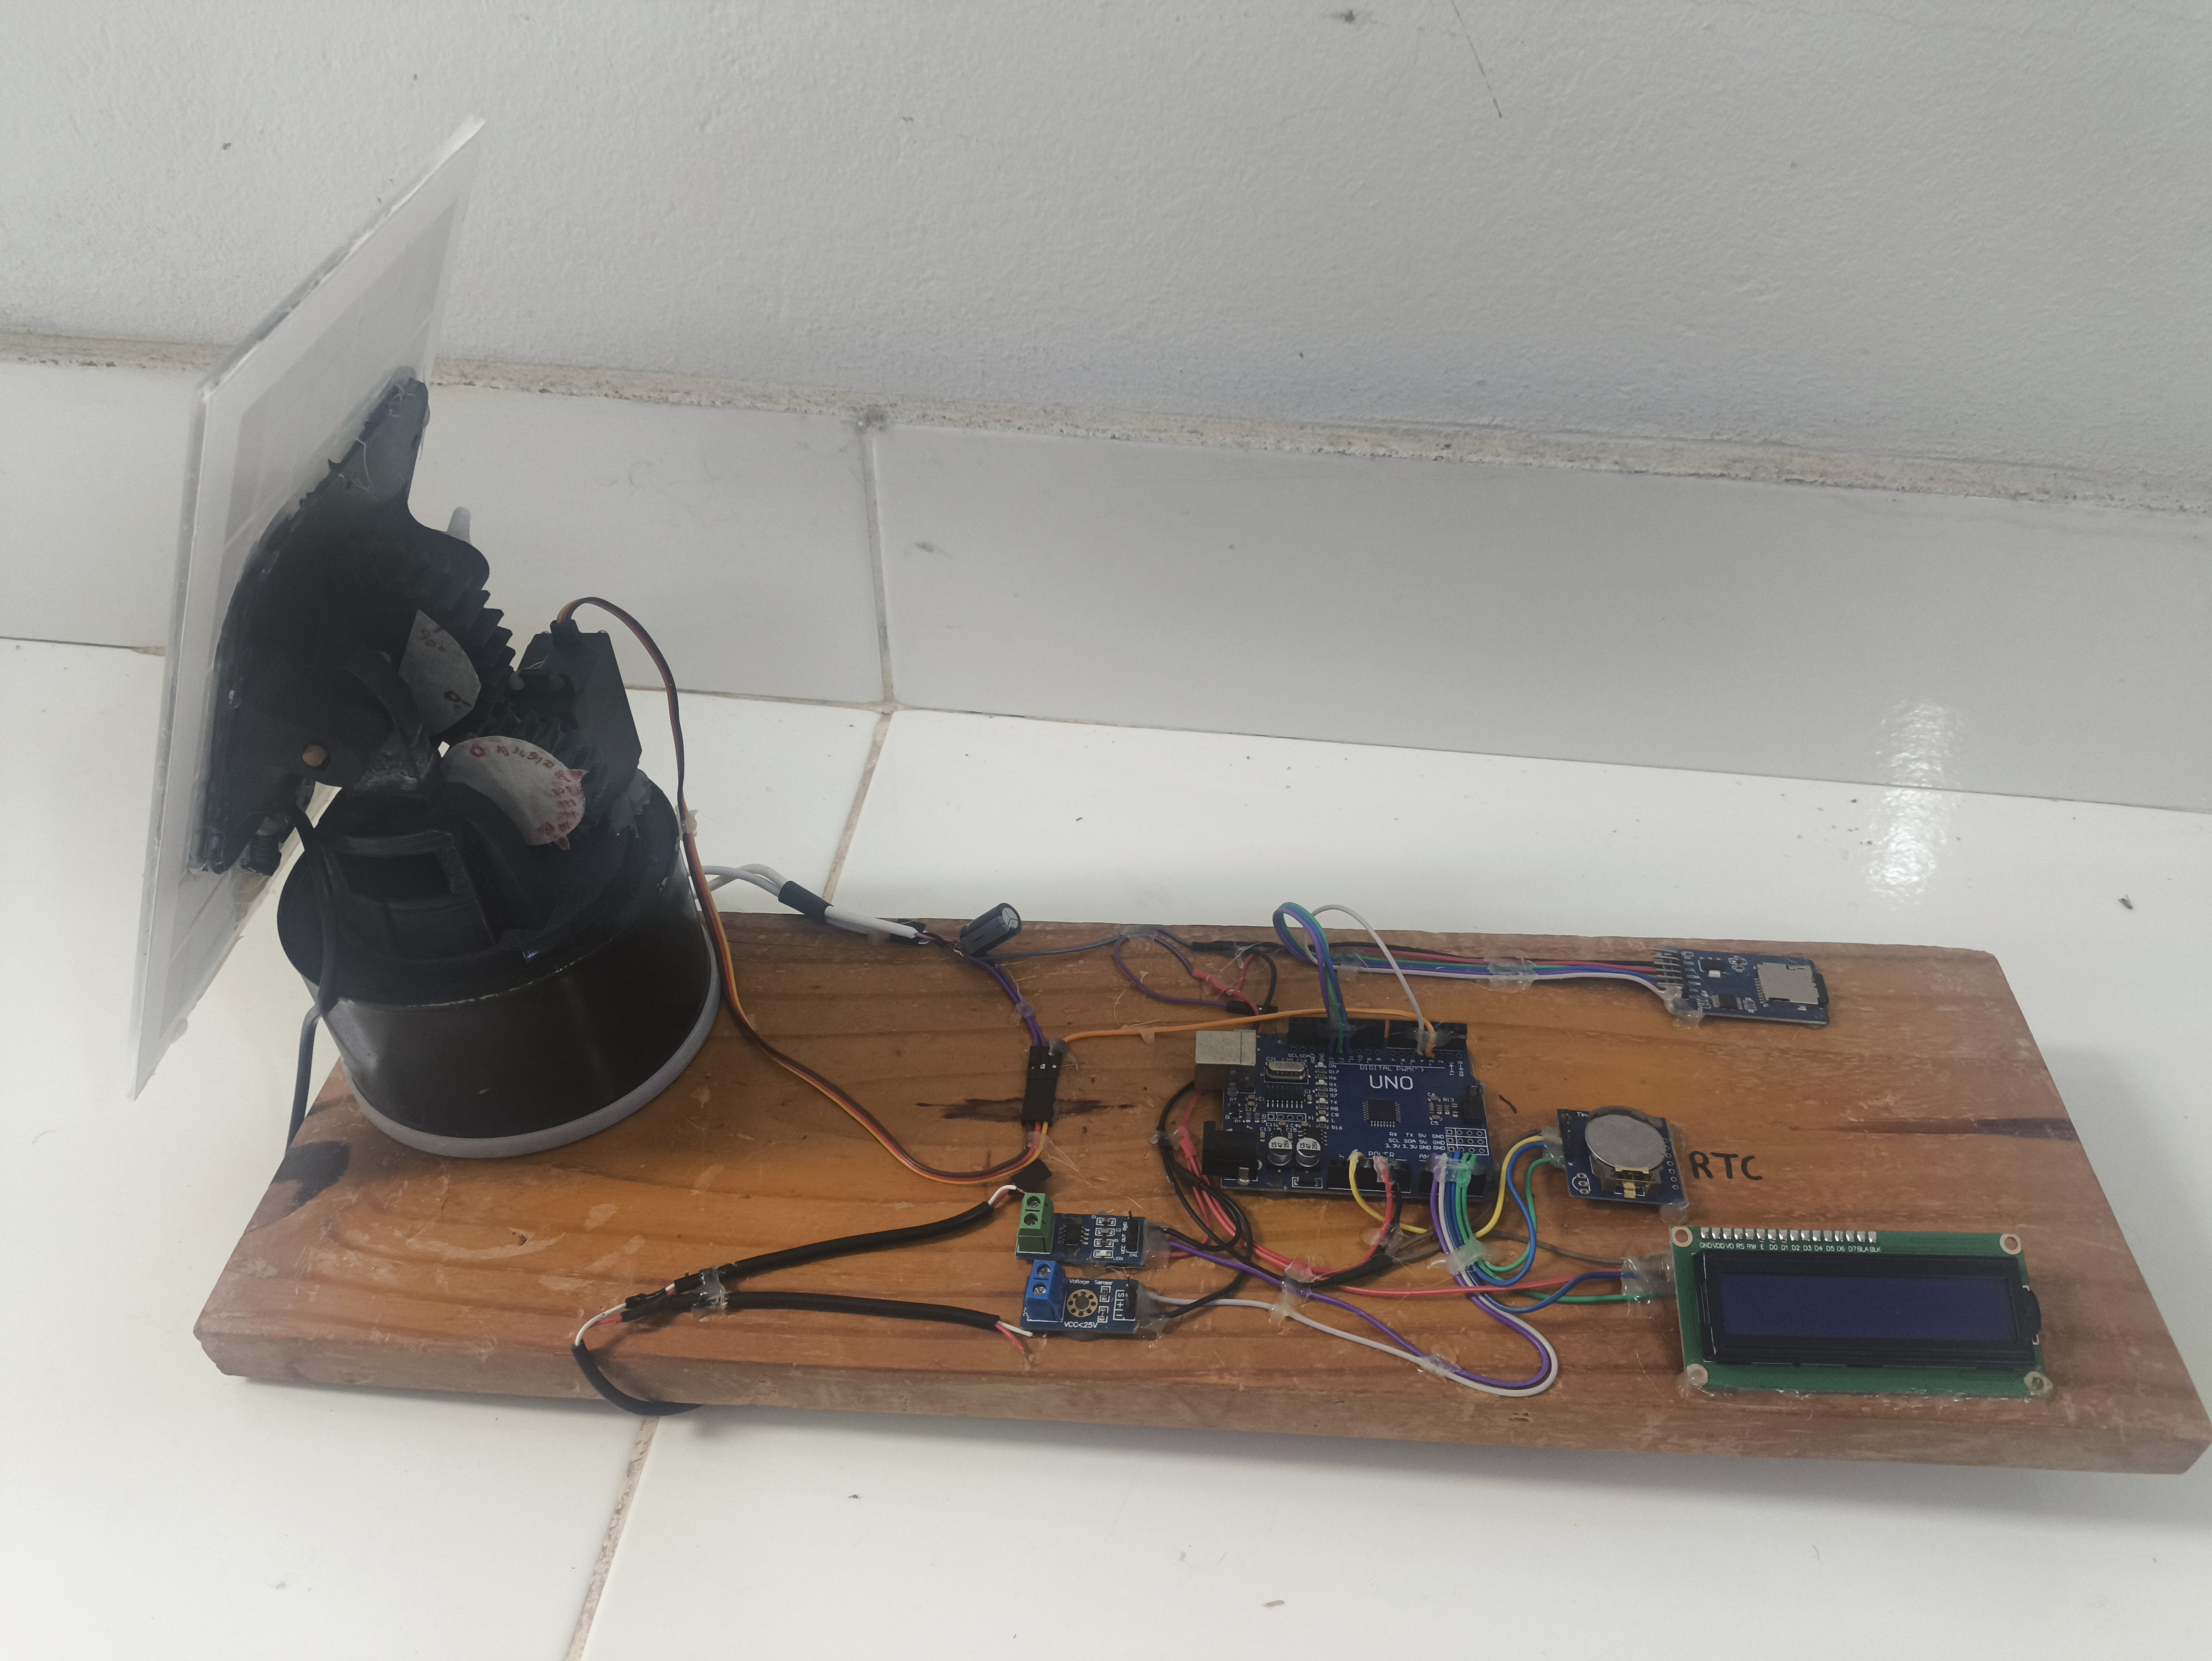
\includegraphics[width=0.6\linewidth]{Figuras/prototipo_montado.jpg}
    \caption{Protótipo do sistema automatizado desenvolvido}
    \label{fig:prototipo_montado}
    \legend{Fonte: Autor (2026).}
\end{figure}

O movimento realizado pelo servo motor corresponde à rotação do sistema em torno de um único eixo, estando diretamente associado ao deslocamento aparente do Sol no céu, no sentido Leste–Oeste. Esse movimento constitui o princípio de funcionamento do sistema automatizado de eixo único desenvolvido neste trabalho, permitindo maximizar a incidência de radiação solar sobre o painel fotovoltaico ao longo do dia.

Durante o desenvolvimento da estrutura mecânica, foram priorizados critérios como simplicidade construtiva, baixo custo, robustez e facilidade de manutenção, considerados essenciais para a viabilidade prática da proposta. Além disso, buscou-se minimizar folgas mecânicas e desalinhamentos que pudessem comprometer a precisão do sistema.

Posteriormente, foi implementada uma estrutura de isolamento ao redor do protótipo, com o objetivo de proteger os componentes eletrônicos contra intempéries, como chuva e umidade, bem como contra a incidência direta de radiação solar e possíveis interferências externas, como a presença de aves. Tais condições poderiam ocasionar danos aos componentes eletrônicos e comprometer a confiabilidade da coleta de dados. A solução adotada é apresentada na Figura~\ref{fig:protecao_prototipo}.

\begin{figure}[H]
    \centering
    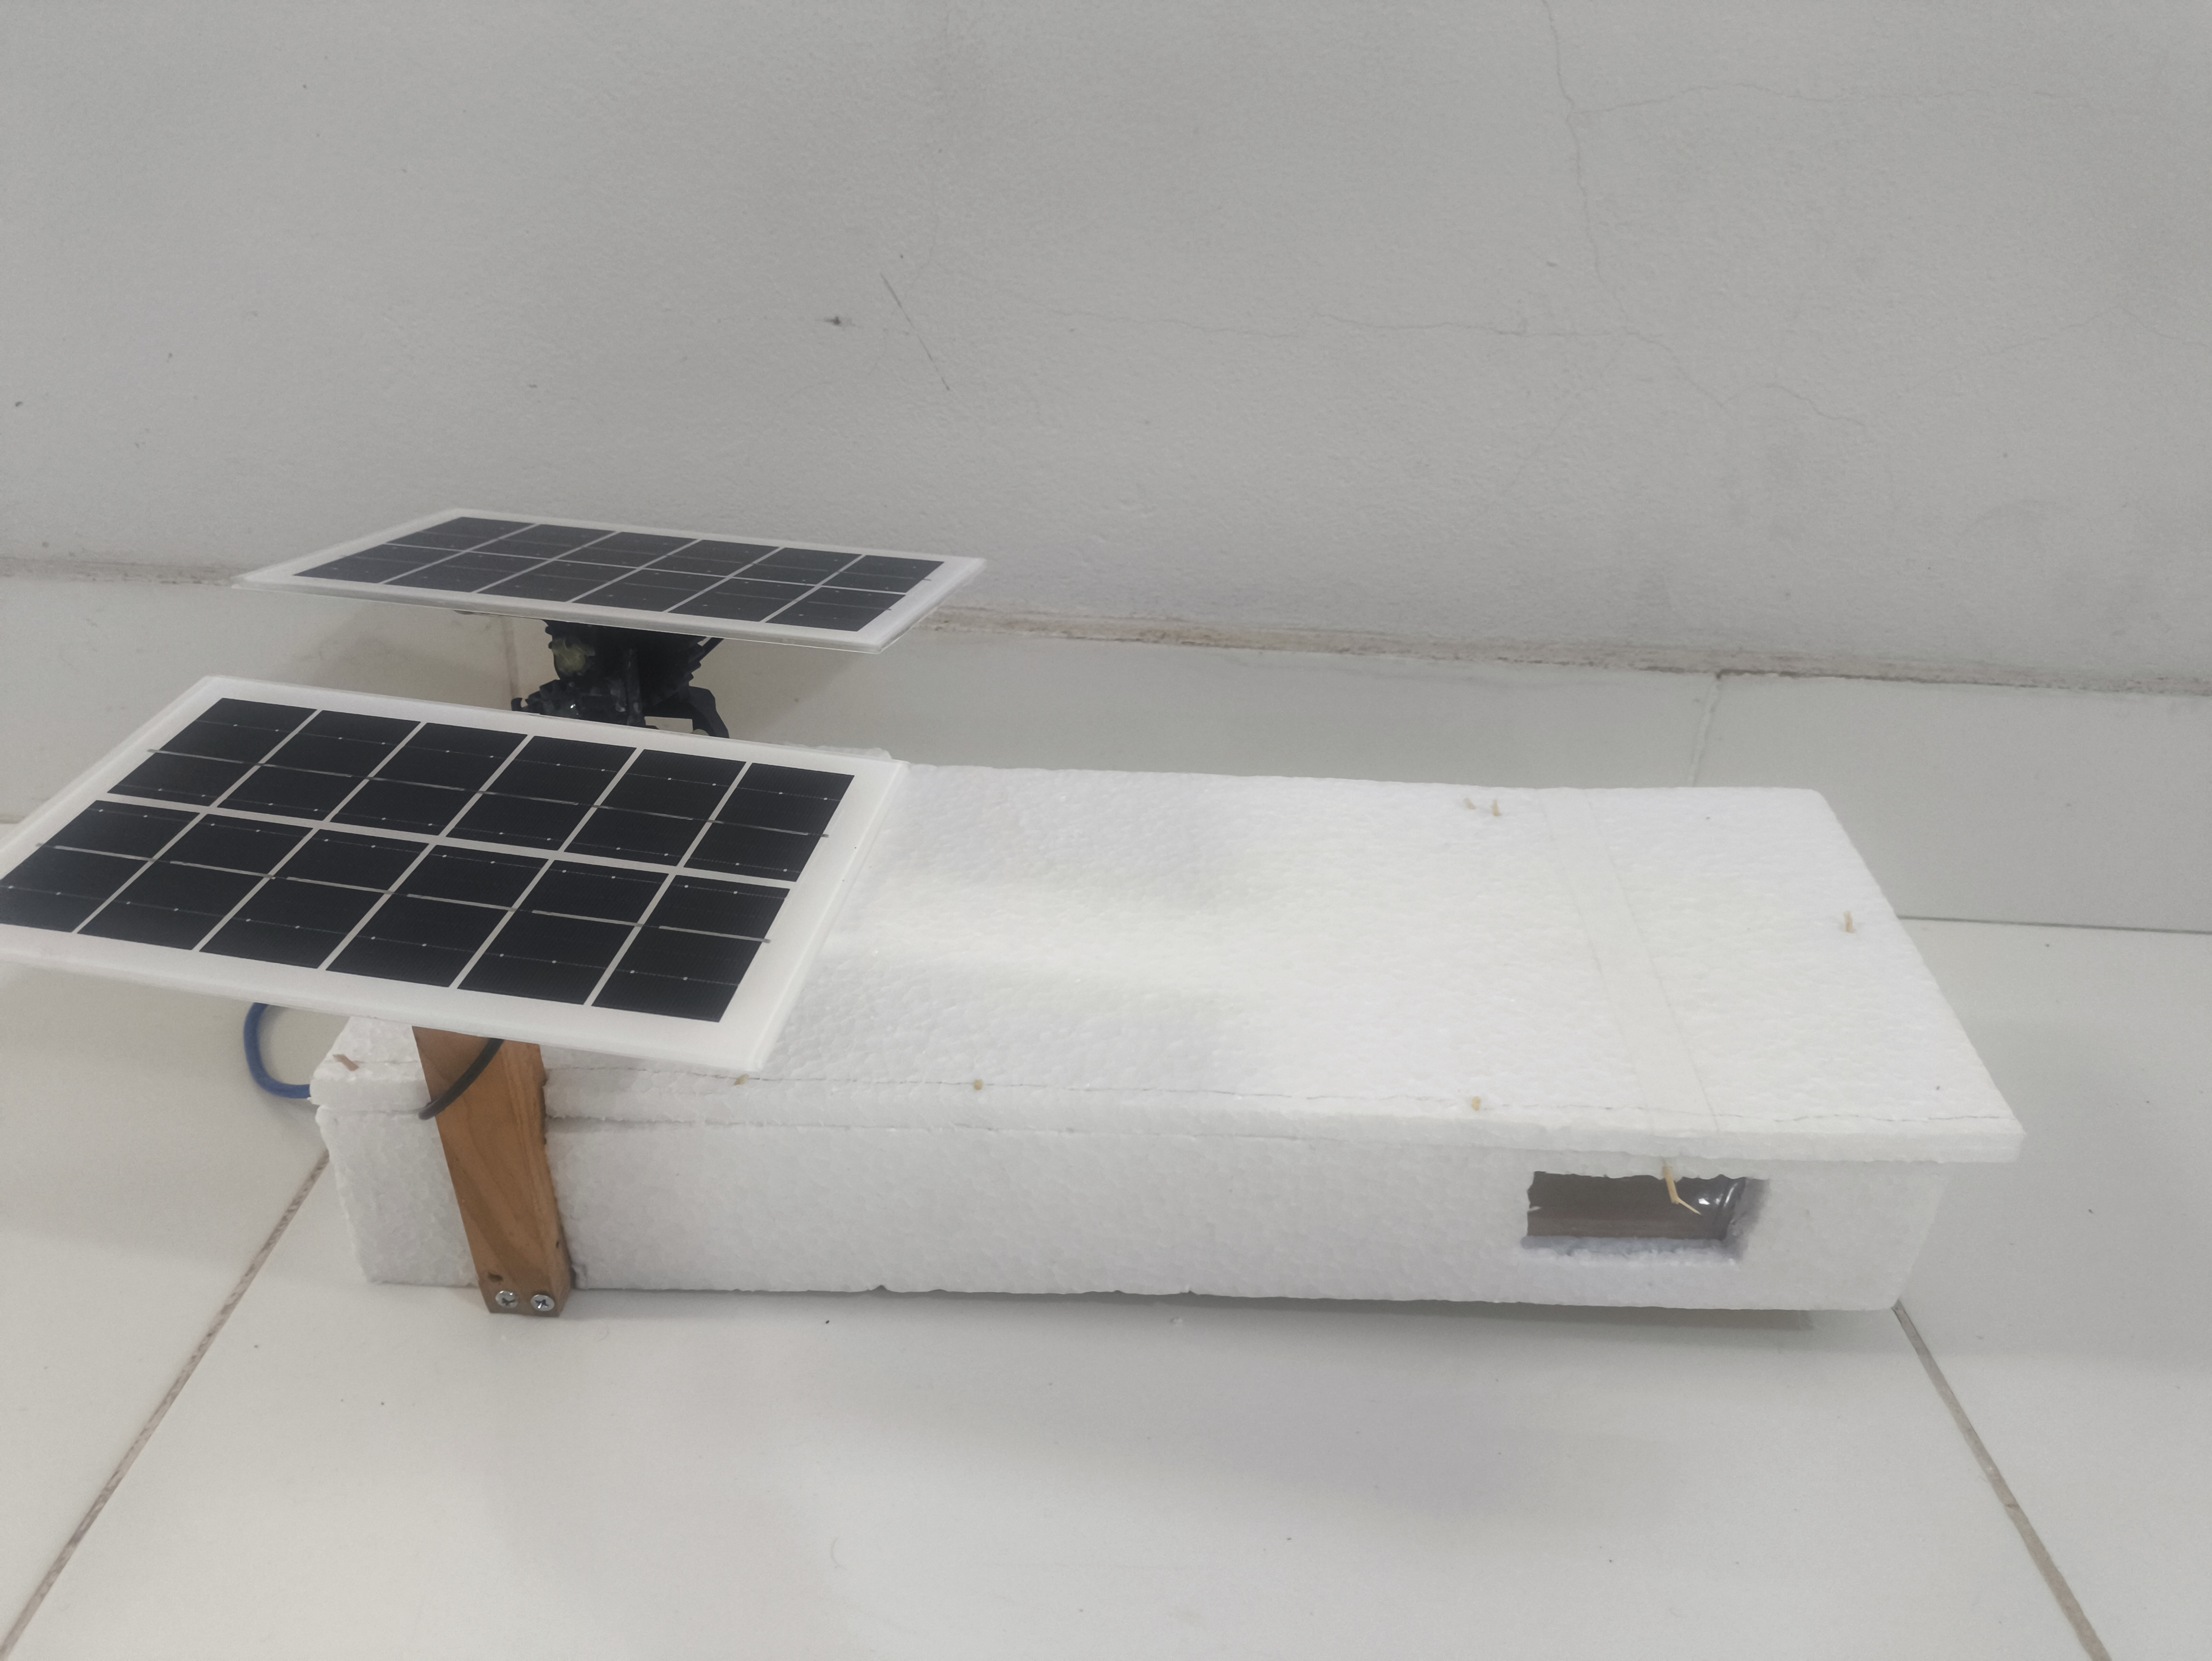
\includegraphics[width=0.7\linewidth]{Figuras/proteçao_prototipo.jpg}
    \caption{Estrutura de proteção do protótipo}
    \legend{Fonte: Autor (2026)}
    \label{fig:protecao_prototipo}
\end{figure}
\vspace{-0.4cm}
A seguir, serão apresentados os componentes utilizados na construção do sistema.
\vspace{-0.4cm}

\subsection{Arduino Uno}


Para atuar como controlador do sistema, foi selecionado o Arduino Uno, em razão de sua ampla utilização, robustez e extensa documentação disponível, fatores que facilitam sua aplicação em projetos acadêmicos e de prototipagem. O Arduino Uno é uma placa de microcontrolador baseada no ATmega328P, que possui 14 pinos de entrada e saída digitais, dos quais 6 podem ser utilizados como saídas Pulse Width Modulation (PWM), além de entradas analógicas que permitem a leitura de sinais provenientes de sensores \cite{arduino2023}.
conforme apresentado na Figura \ref{fig:arduino_uno}.
\begin{figure}[H]
    \centering
    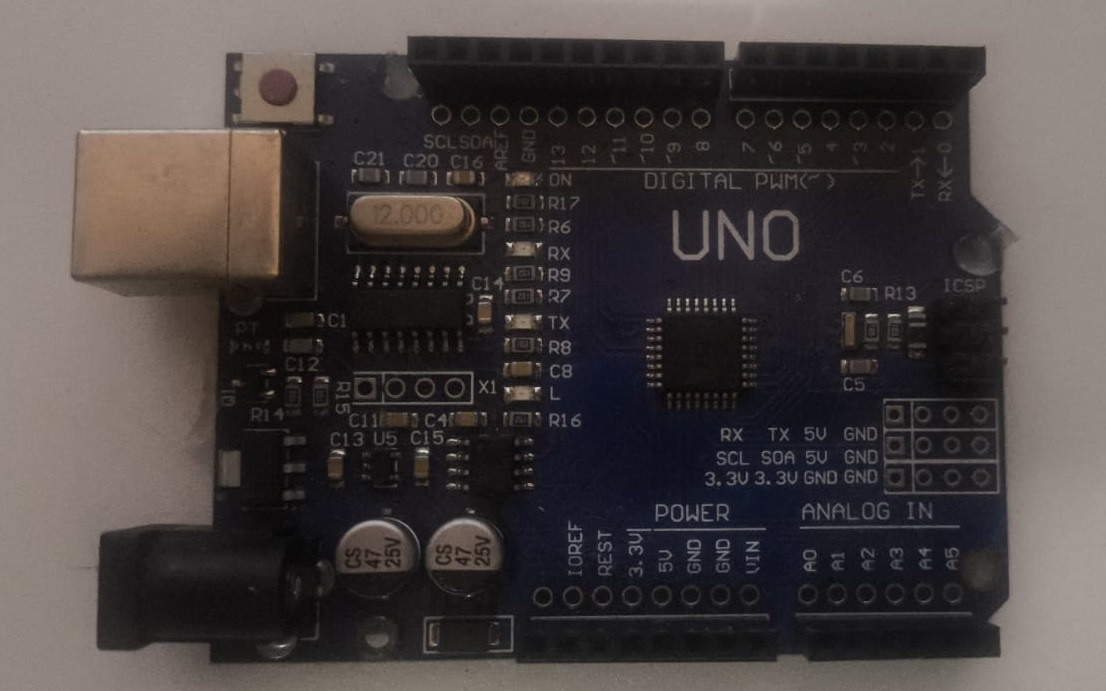
\includegraphics[width=0.6\textwidth]{Figuras/Placa Arduino Uno.jpeg}
    \caption{Placa Arduino Uno}
    \caption*{Fonte: Autor (2026).}
    \label{fig:arduino_uno}
\end{figure}


A placa reúne os recursos necessários para o desenvolvimento de sistemas embarcados, oferecendo suporte adequado à integração entre sensores, atuadores e módulos de comunicação. Sua arquitetura simplificada, aliada ao ambiente de desenvolvimento integrado, permite a programação em linguagem baseada em C e C++, contribuindo para a implementação eficiente da lógica de controle do sistema.

No contexto deste trabalho, o Arduino Uno desempenha papel central no processamento das informações, sendo responsável pela aquisição dos dados provenientes dos sensores utilizados. A partir desses dados, o microcontrolador executa rotinas programadas que determinam o posicionamento angular adequado do painel fotovoltaico ao longo do dia, com base na trajetória aparente do Sol.

Adicionalmente, o Arduino realiza o envio de sinais de controle ao atuador responsável pelo ajuste da inclinação do painel, garantindo o acompanhamento contínuo da posição solar. Paralelamente, o sistema executa o gerenciamento e o registro dos dados coletados, armazenando informações como tensão, corrente, potência e posição angular, o que possibilita análises posteriores e a validação experimental do desempenho do sistema.

Dessa forma, o Arduino Uno atua como a unidade central de processamento de um sistema embarcado, integrando as etapas de aquisição, processamento, controle e armazenamento de dados em tempo real. Tal aplicação evidencia a utilização de conceitos fundamentais de programação, automação e integração entre hardware e software, essenciais para o desenvolvimento de soluções tecnológicas eficientes e de baixo custo.

\subsection{Servo Motor}

O servo motor utilizado no desenvolvimento do protótipo foi o modelo MG996R, selecionado em razão de suas características de desempenho, como elevado torque, boa precisão de posicionamento e robustez mecânica, aspectos considerados fundamentais para aplicações que exigem controle angular confiável, conforme apresentado na Figura~\ref{fig:servo_mg996r}.

\begin{figure}[H]
    \centering
    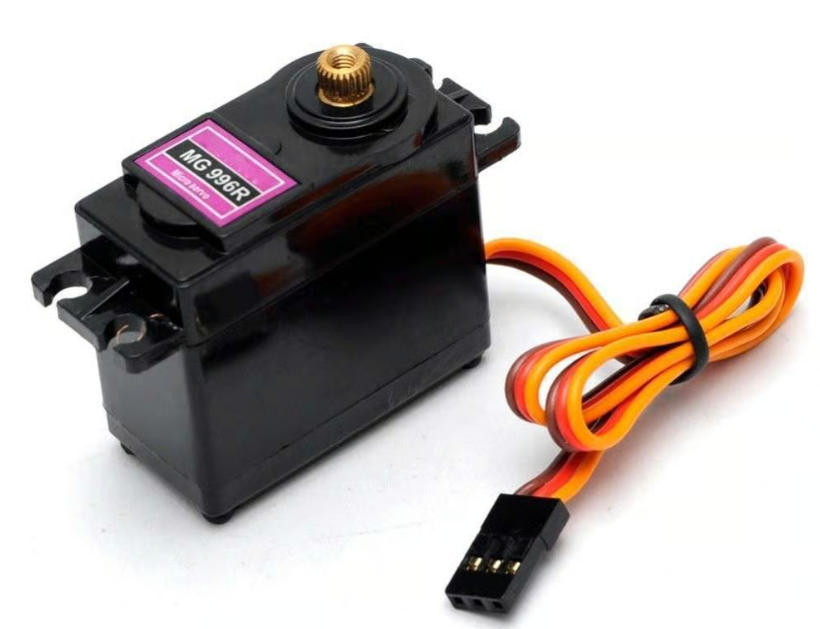
\includegraphics[width=0.6\textwidth]{Figuras/servo motor.png}
    \caption{Servo motor MG996R}
    \caption*{Fonte: Fonte: Adaptado de Eletrônica Castro (2026)}
    \label{fig:servo_mg996r}
\end{figure}

Esse atuador apresenta uma faixa de rotação aproximada de 0° a 180°, sendo constituído por um sistema interno de controle que integra um motor de corrente contínua (DC), um conjunto de engrenagens, um potenciômetro de realimentação e um circuito eletrônico de controle. Esse conjunto permite o posicionamento preciso do eixo em função do sinal de controle recebido, garantindo estabilidade e repetibilidade nos movimentos. Tais características justificam sua ampla aplicação em projetos de robótica, automação e sistemas embarcados \cite{towerpro2019}.

No contexto deste trabalho, o servo motor desempenha a função de elemento de acionamento do sistema, sendo responsável pela movimentação do painel fotovoltaico. O controle do posicionamento angular é realizado pelo Arduino por meio de sinais PWM, nos quais a largura do pulso está diretamente relacionada ao ângulo desejado, permitindo o posicionamento preciso do servomotor \cite{arduino_servo}. Dessa forma, o sistema ajusta continuamente a inclinação do painel com base nas informações de tempo fornecidas pelo sistema, possibilitando o acompanhamento da trajetória aparente do Sol ao longo do dia.

A precisão no posicionamento angular constitui um fator determinante para o desempenho do sistema, uma vez que influencia diretamente a incidência da radiação solar sobre o painel e, consequentemente, a eficiência na geração de energia. Além disso, a capacidade do servo motor de realizar movimentos suaves e controlados contribui para a redução de vibrações, a minimização de esforços mecânicos e o aumento da vida útil dos componentes estruturais.

Dessa forma, a utilização do servo motor MG996R mostrou-se adequada à proposta do projeto, atendendo aos requisitos de torque, precisão, confiabilidade e custo, essenciais para o desenvolvimento de um protótipo funcional automatizado.

\subsection{Placa Solar Fotovoltaica}

Para a realização dos experimentos, foi utilizada uma placa solar fotovoltaica de pequeno porte, com potência nominal de 3 W (watt) e tensão de saída de 6 V (volt) em corrente contínua. O módulo apresenta dimensões aproximadas de 21~cm $\times$ 13~cm e é constituído por células do tipo policristalino, tecnologia amplamente empregada em sistemas fotovoltaicos devido ao seu bom custo-benefício e confiabilidade, conforme apresentado na Figura~\ref{fig:placa_solar}.

\begin{figure}[H]
    \centering
    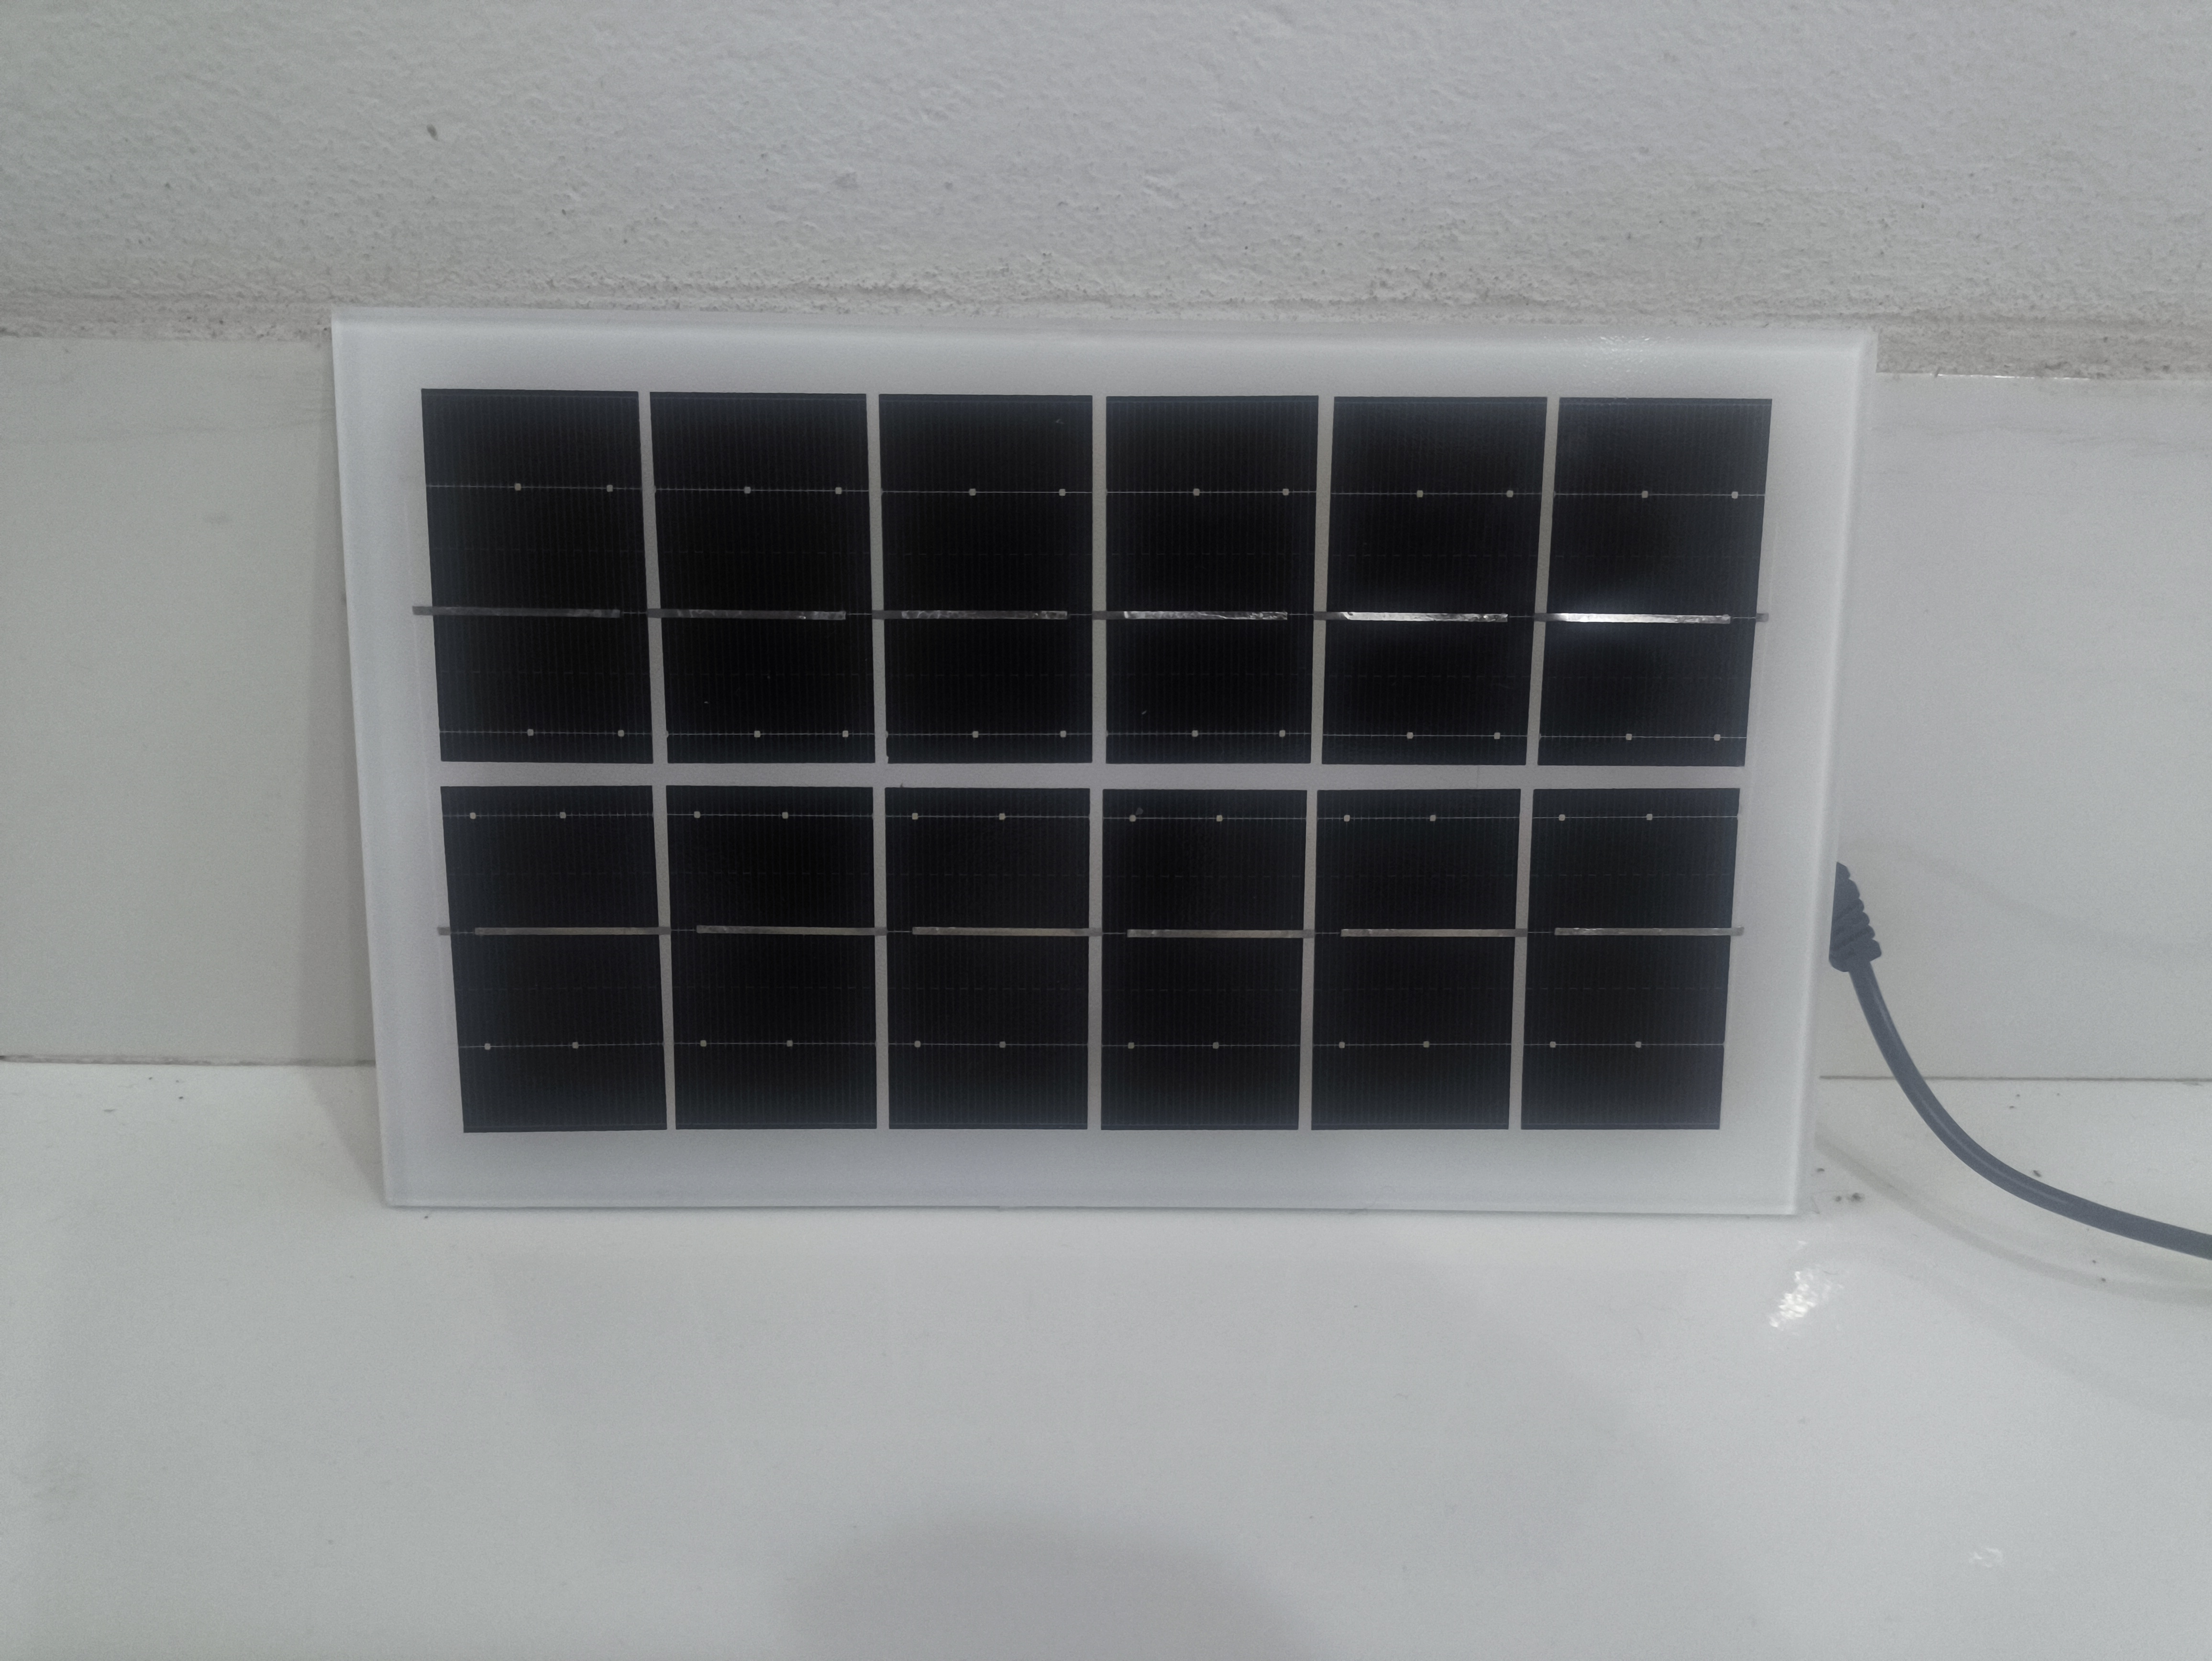
\includegraphics[width=0.7\textwidth]{Figuras/placa_solar.jpg}
    \caption{Placa solar fotovoltaica utilizada no experimento}
    \caption*{Fonte: Autor (2026).}
    \label{fig:placa_solar}
\end{figure}

O painel fotovoltaico é o elemento responsável pela conversão da energia solar em energia elétrica, sendo utilizado neste trabalho como fonte de dados para a análise do desempenho do sistema. Embora apresente capacidade de geração reduzida, sua aplicação mostra-se adequada aos objetivos propostos, uma vez que permite avaliar, de forma comparativa, o ganho percentual de eficiência proporcionado pelo sistema automatizado em relação a um sistema de eixo fixo.

A geração de energia de um painel fotovoltaico depende diretamente das condições ambientais, como temperatura e irradiância solar. Os testes e a avaliação de desempenho desses módulos são realizados com base em condições padronizadas e controladas, podendo ocorrer variações significativas na geração de energia quando tais condições não são atendidas. Nesse contexto, destacam-se as Condições Padrão de Teste (\textit{Standard Test Conditions} — STC), utilizadas como referência para a avaliação do desempenho dos módulos. Nessas condições, considera-se uma irradiância de 1000 W/m², temperatura da célula de 25~°C e espectro solar padrão, cenário no qual o painel opera próximo à sua potência nominal \cite{iec2016}.

Considerando essas premissas, mesmo com a utilização de um módulo de baixa potência, é possível obter dados experimentais consistentes para a análise do comportamento do sistema, permitindo a validação da proposta e a quantificação dos ganhos energéticos proporcionados pela automação.

\subsection{Módulo Sensor de Corrente e Sensor de Tensão}

Para a aquisição de dados elétricos do sistema, foram utilizados sensores de corrente e de tensão, elementos fundamentais para o monitoramento e avaliação do desempenho do painel fotovoltaico, conforme apresentado na Figura \ref{fig:sensores}.

\begin{figure}[H]
    \centering

    \begin{minipage}{0.45\linewidth}
        \centering
        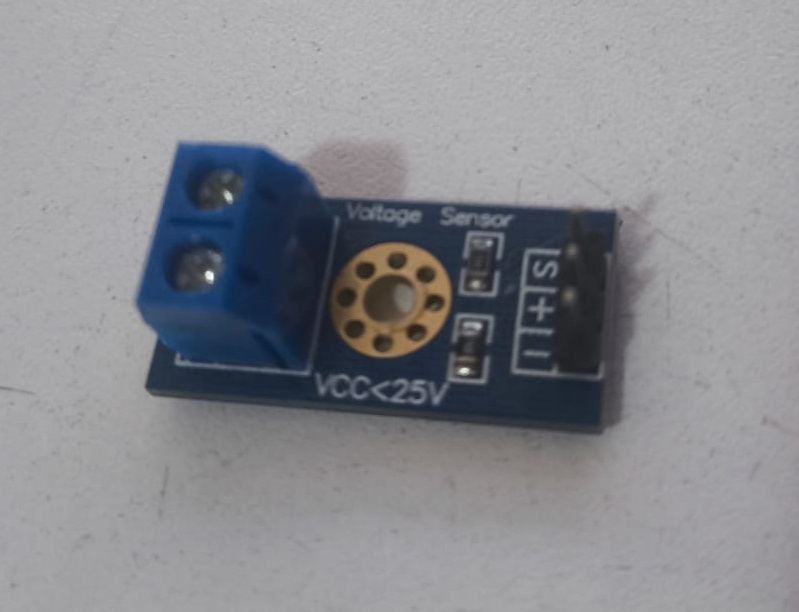
\includegraphics[height=5cm]{Figuras/sensor_tensao.jpeg}
        
        (a) Sensor de tensão
    \end{minipage}
    \hfill
    \begin{minipage}{0.45\linewidth}
        \centering
        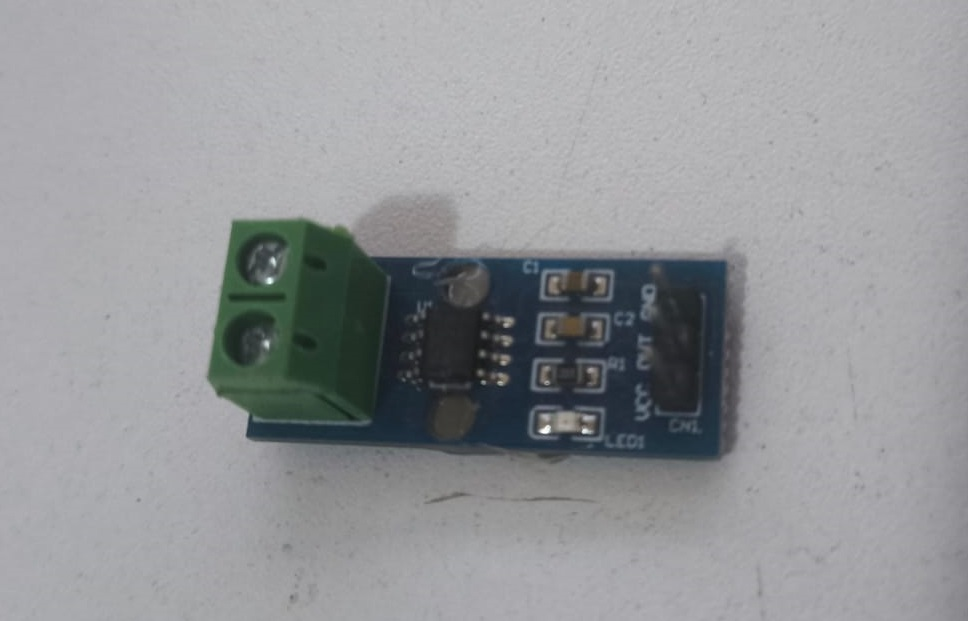
\includegraphics[height=5cm]{Figuras/sensor_corrente.jpeg}
        
        (b) Sensor de corrente
    \end{minipage}

    \caption{Sensores utilizados para aquisição de dados elétricos}
    \legend{Fonte: Autor (2026).}
    \label{fig:sensores}
\end{figure}


O sensor de corrente empregado foi o modelo ACS712, disponível em diferentes faixas de medição, como 5 A, 20 A e 30 A, sendo capaz de medir tanto corrente contínua quanto alternada. Esse dispositivo é baseado no efeito Hall, no qual a passagem de corrente elétrica por um condutor interno gera um campo magnético proporcional, detectado por um circuito integrado, permitindo a medição indireta da corrente elétrica \cite{allegro2019}.

O funcionamento do ACS712 baseia-se na conversão da corrente elétrica em um sinal de tensão analógico proporcional, geralmente centrado em torno de metade da tensão de alimentação do sensor. Essa característica permite ao microcontrolador interpretar tanto correntes positivas quanto negativas. Além disso, o sensor apresenta boa linearidade, isolamento elétrico entre o circuito de potência e o circuito de medição, bem como resposta rápida, o que o torna adequado para aplicações em sistemas embarcados e de monitoramento energético \cite{sparkfun_acs712}.

No contexto deste trabalho, o sensor de corrente é responsável por medir a intensidade da corrente gerada pelo painel fotovoltaico ao longo do dia, possibilitando a análise do comportamento do sistema sob diferentes condições de irradiância e posicionamento angular.

Complementarmente, foi utilizado um sensor de tensão baseado no princípio do divisor resistivo, com faixa de medição de até 25 V em corrente contínua. Esse módulo reduz a tensão de entrada para níveis compatíveis com as entradas analógicas do Arduino, garantindo a integridade do microcontrolador durante a aquisição dos dados \cite{usinainfo2024}.

A partir dos dados coletados pelos sensores de corrente e tensão, o sistema realiza o cálculo da potência elétrica instantânea gerada pelo painel fotovoltaico. Essa potência representa a taxa de conversão de energia elétrica em um determinado instante e é obtida conforme a relação fundamental entre essas grandezas:

\[
P = V \cdot I
\]

em que \(P\) representa a potência elétrica (em watts), \(V\) a tensão elétrica (em volts) e \(I\) a corrente elétrica (em amperes).

Essa relação indica que a potência gerada pelo sistema depende simultaneamente da tensão fornecida pelo painel e da corrente que circula no circuito. Dessa forma, variações nas condições ambientais, como irradiância e temperatura, influenciam diretamente essas grandezas. O sensor de tensão utilizado baseia-se no princípio do divisor de tensão resistivo, permitindo a redução de níveis de tensão mais elevados para valores compatíveis com a entrada analógica do microcontrolador \cite{sedra2016}. As medições obtidas permitem não apenas o cálculo da potência instantânea, mas também a análise do desempenho energético ao longo do tempo, sendo essenciais para a comparação entre o sistema automatizado e o sistema de eixo fixo.

Os sensores de corrente e tensão atuam, portanto, como dispositivos de aquisição de dados do sistema, permitindo a conversão de grandezas físicas em sinais elétricos interpretáveis pelo microcontrolador. Os dados obtidos são posteriormente processados, armazenados e utilizados na geração de indicadores de desempenho, evidenciando a integração entre hardware e software no desenvolvimento do sistema proposto e possibilitando a validação experimental dos resultados obtidos em simulação.

\subsection{Módulo Real Time Clock (RTC) DS1307}

Para a obtenção de informações temporais no sistema, foi utilizado o módulo \textit{Real Time Clock} (RTC), modelo DS1307, um dispositivo eletrônico dedicado à contagem contínua do tempo, capaz de manter seu funcionamento mesmo na ausência de alimentação principal, por meio de uma bateria auxiliar, conforme apresentado na Figura~\ref{fig:rtc}.

\begin{figure}[H]
    \centering
    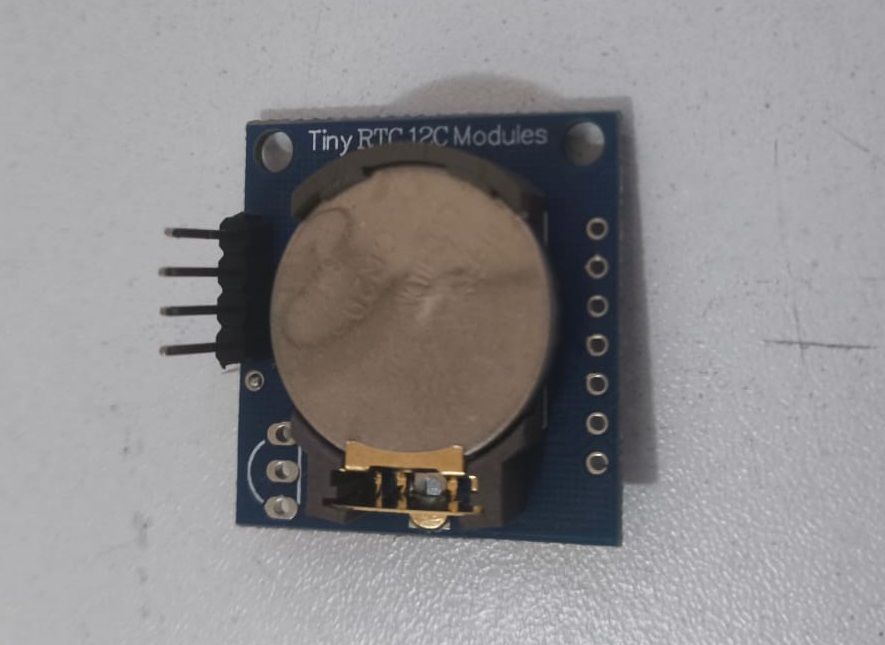
\includegraphics[width=0.6\textwidth]{Figuras/rtc.jpeg}
    \caption{Módulo RTC DS1307 utilizado no sistema}
    \caption*{Fonte: Autor (2026).}
    \label{fig:rtc}
\end{figure}

O DS1307 dispõe de um calendário completo, fornecendo dados de segundos, minutos, horas, dia da semana, data, mês e ano. A comunicação com o microcontrolador é realizada por meio do protocolo I2C (\textit{Inter-Integrated Circuit}), o que permite uma integração eficiente com plataformas embarcadas, como o Arduino, utilizando apenas duas linhas de comunicação (SDA e SCL) \cite{maxim2015}.

O dispositivo possui um circuito interno de detecção de falhas de energia (\textit{power-fail detect}), responsável pela comutação automática entre a alimentação principal e a bateria de backup, garantindo a continuidade da contagem do tempo e evitando a perda de dados temporais, o que o torna essencial em aplicações que exigem registro contínuo e confiável de informações \cite{maxim2015}.

Além disso, os dados fornecidos pelo RTC são fundamentais para o processo de aquisição e registro de dados experimentais. Cada leitura de tensão, corrente e potência é associada a um instante específico de tempo, permitindo a construção de séries temporais para análise do desempenho energético do sistema. Essa abordagem possibilita a comparação detalhada entre os sistemas, tanto em termos instantâneos quanto acumulados ao longo do dia.

Dessa forma, o módulo RTC DS1307 pode ser compreendido como um componente essencial para a organização temporal e sincronização dos dados, contribuindo diretamente para a confiabilidade das análises e para a validação experimental dos resultados obtidos.

\subsection{Módulo Leitor de Cartão Micro SD}

Para a gravação e armazenamento dos dados obtidos durante a execução do sistema, foi utilizado um módulo leitor de cartão microSD, responsável pela persistência das informações geradas ao longo do funcionamento do protótipo. Esse módulo permite o armazenamento dos dados em arquivos no formato texto, facilitando a posterior análise e visualização em softwares de planilhas eletrônicas, conforme apresentado na Figura~\ref{fig:sd}.

\begin{figure}[H]
    \centering
    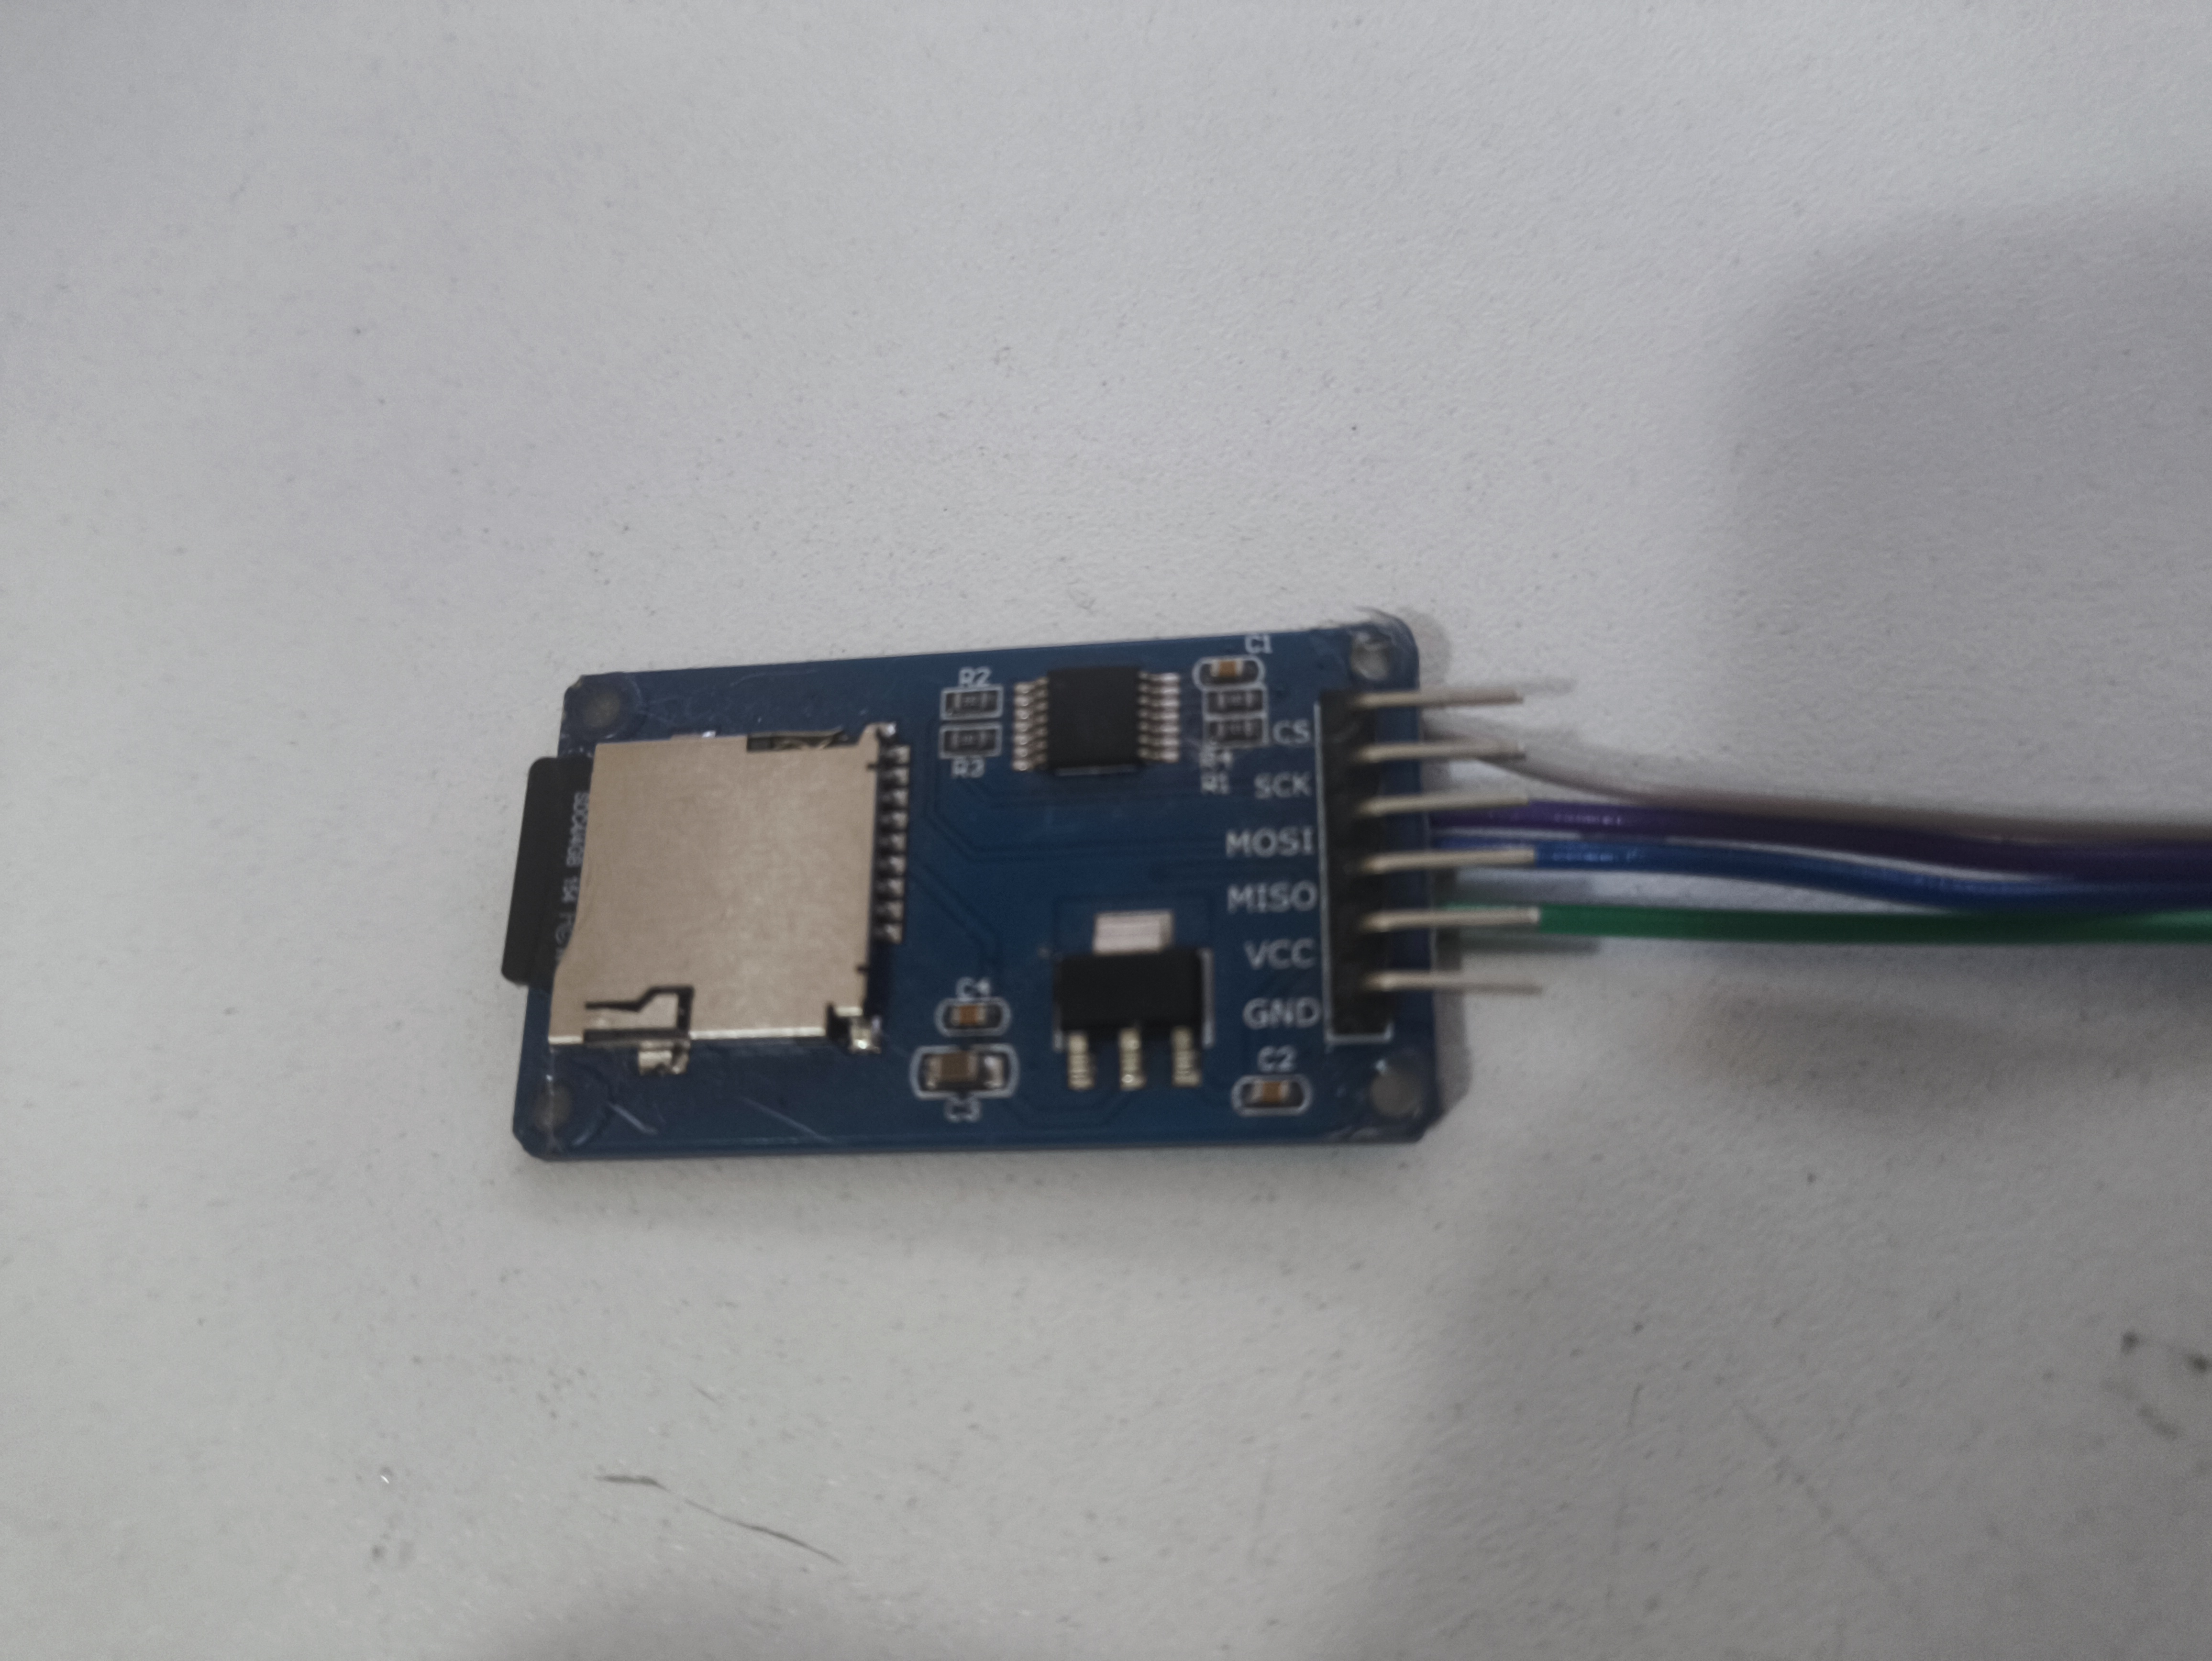
\includegraphics[width=0.6\textwidth]{Figuras/cartao_sd.jpg}
    \caption{Módulo leitor de cartão micro SD utilizado no sistema}
    \caption*{Fonte: Autor (2026).}
    \label{fig:sd}
\end{figure}

O módulo consiste em um dispositivo que integra um leitor de cartão microSD, permitindo a leitura e escrita de dados por meio de comunicação com o microcontrolador. Sua utilização é amplamente difundida em sistemas embarcados, especialmente em aplicações que demandam o registro contínuo de informações para análises posteriores, possibilitando o armazenamento organizado dos dados em arquivos digitais, como .txt ou .csv, o que facilita sua posterior análise em softwares de processamento de dados \cite{eletrogate2022}.

No contexto deste trabalho, o módulo é responsável pelo armazenamento estruturado dos dados coletados pelo sistema. Entre as variáveis registradas, destacam-se data, hora, tensão, corrente, potência elétrica e o ângulo de posicionamento do painel fotovoltaico. Esses dados são organizados em arquivos no cartão de memória, geralmente em formato texto (.txt) ou (.csv), o que facilita a posterior importação e análise em softwares como planilhas eletrônicas e ambientes de simulação.

Essa abordagem possibilita a construção de séries temporais detalhadas, fundamentais para a análise do comportamento energético do sistema. A partir desses dados, é possível calcular parâmetros como potência instantânea, energia acumulada e eficiência relativa, permitindo uma comparação consistente entre o sistema automatizado solar e o sistema de eixo fixo.

O módulo de cartão microSD desempenha, portanto, um papel essencial na etapa de persistência dos dados, assegurando a integridade,e a disponibilidade e a rastreabilidade das informações coletadas. Dessa forma, viabilizam-se análises quantitativas mais robustas e a validação experimental dos resultados obtidos.

\subsection{display de cristal líquido (Liquid Crystal Display – LCD)}

Para a visualização das informações do sistema, foi utilizado um display LCD 16x2 com interface I2C, que atua como meio de comunicação entre o sistema embarcado e o usuário. Esse tipo de display permite a exibição de caracteres alfanuméricos distribuídos em duas linhas de 16 colunas, sendo amplamente empregado em aplicações embarcadas devido à sua simplicidade, baixo custo e eficiência na apresentação de dados \cite{makerhero2022}, conforme apresentado na Figura~\ref{fig:lcd}.

\begin{figure}[H]
    \centering
    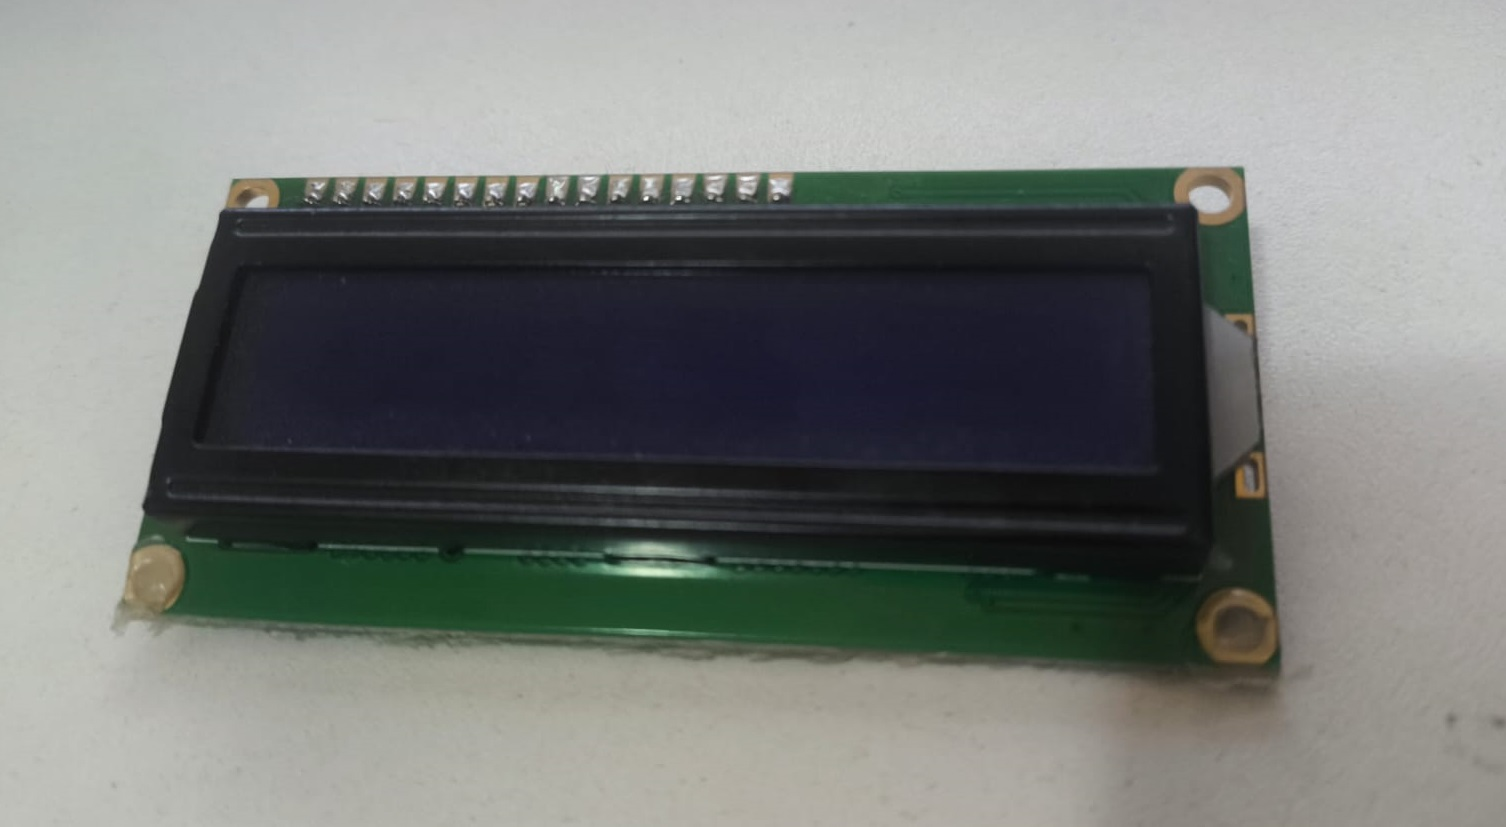
\includegraphics[width=0.6\textwidth]{Figuras/display.jpeg}
    \caption{Display LCD 16x2 com interface I2C utilizado no sistema}
    \caption*{Fonte: Autor (2026).}
    \label{fig:lcd}
\end{figure}


No contexto deste trabalho, o display LCD é utilizado para o monitoramento em tempo real do sistema automatizado, permitindo a visualização contínua das principais variáveis operacionais. Entre as informações exibidas, destacam-se a data e hora no formato DD/MM HH:MM, bem como as grandezas elétricas medidas, incluindo tensão (V), corrente (I), potência (P) e o ângulo de posicionamento do painel fotovoltaico (ANG).

Além da exibição dos dados de operação, o display também desempenha a função de indicar o estado do sistema, podendo apresentar mensagens de inicialização, funcionamento normal e possíveis condições de erro, como falhas na leitura de sensores ou na comunicação com módulos periféricos. Essa funcionalidade contribui para a validação prática do funcionamento do protótipo e auxilia na identificação de inconsistências durante os testes experimentais.

O display LCD 16x2 atua, portanto, como uma interface de saída fundamental no sistema, sendo responsável por apresentar, de forma clara, organizada e em tempo real, os dados processados pelo microcontrolador. Dessa forma, possibilita-se o acompanhamento contínuo das variáveis monitoradas, além de fornecer suporte à análise experimental e à verificação do desempenho do sistema desenvolvido.

\subsection{Programação do Sistema}

A programação do sistema foi desenvolvida utilizando o ambiente Arduino IDE (\textit{Integrated Development Environment}), disponibilizado gratuitamente pela plataforma Arduino. Esse ambiente permite a escrita, compilação e gravação de códigos no microcontrolador de forma simplificada, por meio da conexão da placa ao computador via interface USB. Após a seleção do modelo de placa e da porta de comunicação no ambiente, o código é transferido para o dispositivo, possibilitando sua execução embarcada \cite{arduinoIDE2026}. conforme apresentado na Figura \ref{fig:arduino_ide}.

\begin{figure}[H]
    \centering
    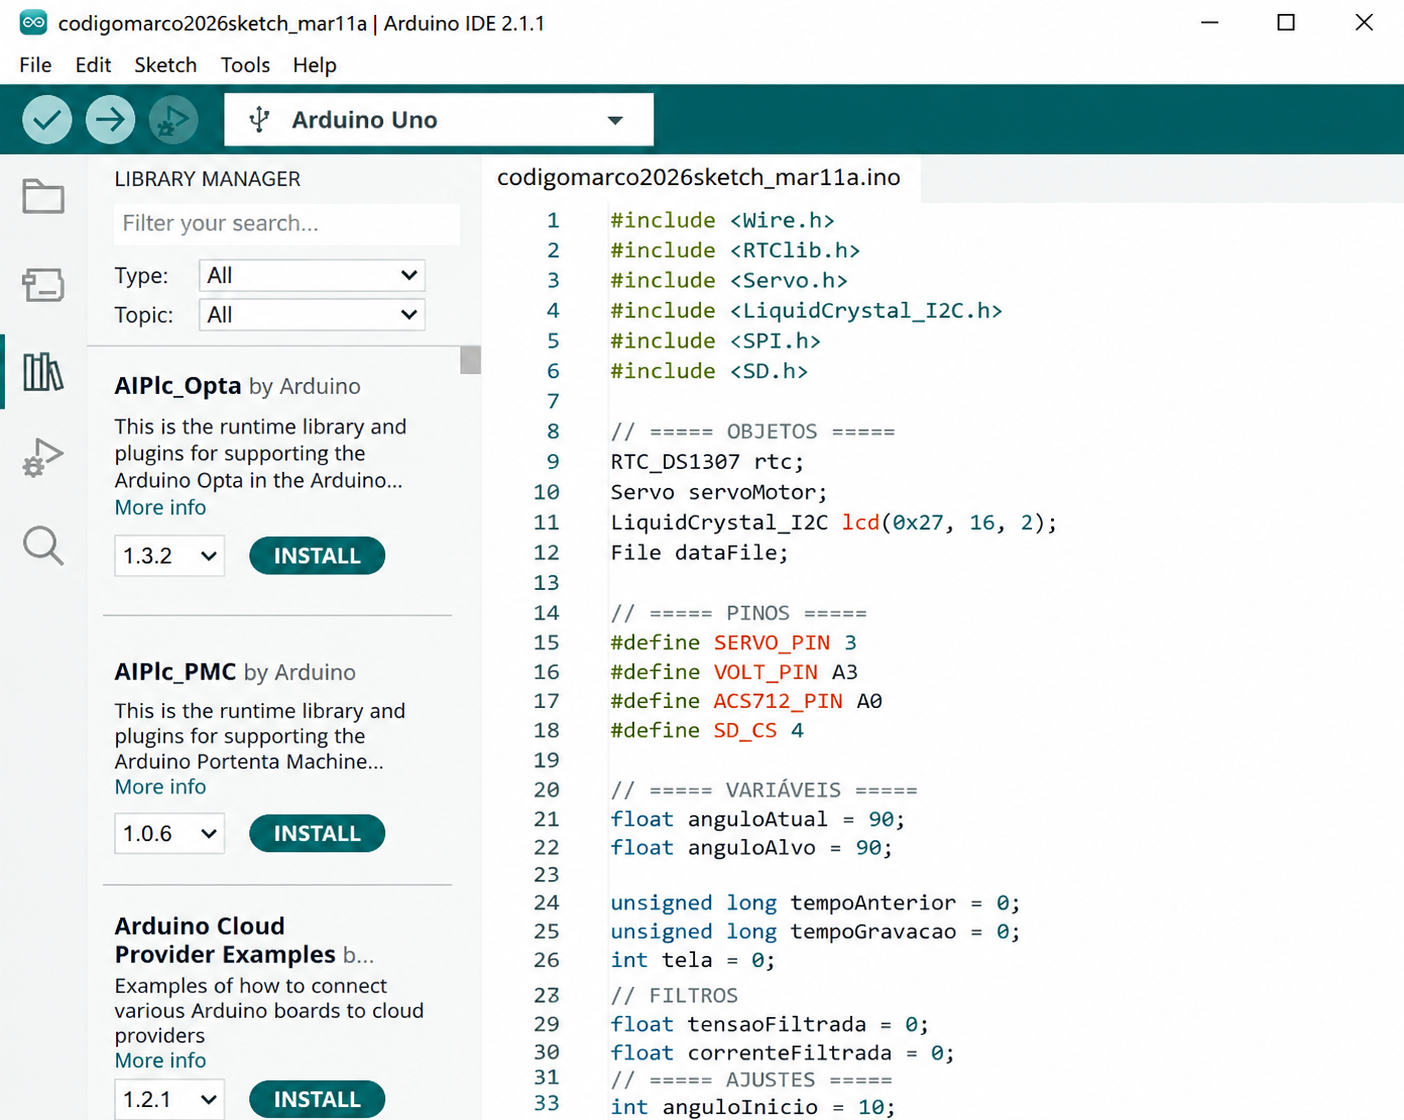
\includegraphics[width=1\textwidth]{Figuras/arduino_ide.png}
    \caption{Ambiente Arduino IDE com o código do sistema automatizado}
    \caption*{Fonte: Autor (2026).}
    \label{fig:arduino_ide}
\end{figure}

Os programas desenvolvidos nesse ambiente são denominados \textit{sketches} e são armazenados com a extensão .ino. Esses arquivos são estruturados, principalmente, em duas funções essenciais: \textit{setup()} e \textit{loop()}. A função \textit{setup()} é executada uma única vez e é responsável pela inicialização dos componentes e configurações do sistema, enquanto a função \textit{loop()} é executada continuamente, garantindo a operação cíclica do sistema ao longo do tempo \cite{arduinoSketch2026}.

Para viabilizar a comunicação com os dispositivos conectados, foram utilizadas bibliotecas específicas, responsáveis por abstrair detalhes de baixo nível e simplificar a implementação. Entre as principais, destacam-se bibliotecas para controle de servo motor, comunicação I2C (RTC e display LCD) e interface SPI (cartão microSD). O uso dessas bibliotecas contribui para a modularização do código, melhoria da legibilidade e redução da complexidade de desenvolvimento \cite{monk2017}.

No contexto deste trabalho, o software desenvolvido atua como núcleo de controle do sistema, sendo responsável por integrar todas as etapas de funcionamento. Inicialmente, o sistema realiza a leitura dos sensores de tensão e corrente por meio das entradas analógicas do microcontrolador, convertendo os sinais adquiridos em valores elétricos reais. A partir dessas grandezas, é efetuado o cálculo da potência instantânea gerada pelo painel fotovoltaico.

Paralelamente, o módulo RTC fornece as informações de data e hora, as quais são utilizadas como variáveis de entrada para o algoritmo de controle do posicionamento do painel. Com base nesses dados, o sistema determina o ângulo de inclinação adequado para cada instante do dia, enviando sinais de controle ao servo motor por meio de modulação por largura de pulso (PWM).

O software desenvolvido para o sistema automatizado foi implementado em plataforma Arduino e integra as funções de aquisição de dados, processamento, controle de posicionamento, otimização e armazenamento de informações. Seu funcionamento baseia-se inicialmente em um modelo de controle temporal, no qual são definidos parâmetros de referência correspondentes ao ângulo inicial do painel (início do dia), ao ângulo de referência para o meio-dia e ao ângulo final (fim do dia). A partir desses pontos, o sistema realiza uma interpolação do posicionamento ao longo do tempo, proporcionando um movimento suave e contínuo do painel fotovoltaico. Essa estratégia permite que, independentemente do horário em que o sistema seja inicializado, o painel seja automaticamente ajustado para a posição angular correspondente ao instante atual.

Além da automação baseado no horário, o sistema incorpora um algoritmo de otimização destinado a maximizar a geração de energia elétrica do módulo fotovoltaico. Para isso, é empregada uma abordagem empírica inspirada nas técnicas de rastreamento do ponto de máxima potência (\textit{Maximum Power Point Tracking} -- MPPT). Os métodos MPPT têm como objetivo maximizar a potência extraída dos módulos fotovoltaicos por meio do ajuste contínuo do ponto de operação do sistema \cite{Esram2007}. Neste trabalho, esse conceito foi adaptado ao posicionamento mecânico do painel solar, de modo que a busca pelo ponto de máxima potência ocorre por meio da variação do ângulo de posicionamento do módulo.

O algoritmo realiza uma varredura angular discreta em torno da posição estimada do painel, avaliando experimentalmente a potência gerada em cada posição. Com base nas medições obtidas, o sistema identifica o ângulo que proporciona a maior potência instantânea e ajusta o painel para essa condição. Dessa forma, o sistema não se limita apenas ao posicionamento calculado em função do horário, mas também considera o desempenho energético real do sistema, orientando o painel para a direção que resulta na máxima geração de energia disponível naquele instante.

Essa estratégia caracteriza uma adaptação dos princípios dos algoritmos MPPT para o domínio mecânico do sistema, permitindo que responda não apenas à posição teórica do Sol, mas também às condições reais de operação, como variações de irradiância, nebulosidade e pequenas imprecisões de alinhamento.

A estratégia adotada caracteriza-se como uma busca local baseada em dados reais obtidos pelos sensores instalados no sistema. Diferentemente dos métodos convencionais de automação que utilizam exclusivamente modelos astronômicos para determinar a posição do Sol, o algoritmo considera diretamente o desempenho energético do painel fotovoltaico, permitindo compensar fatores ambientais como nebulosidade, reflexões e pequenas imprecisões mecânicas.

Paralelamente às rotinas de controle e otimização, o sistema realiza a aquisição e o registro periódico de dados operacionais. As informações coletadas incluem data, hora, tensão, corrente, potência elétrica e ângulo de posicionamento do painel. Esses dados são armazenados em um cartão microSD, formando uma base de dados estruturada para análises posteriores. Simultaneamente, os valores são exibidos em tempo real em um display LCD, possibilitando o monitoramento imediato do desempenho do sistema durante sua operação.

Dessa forma, o software promove a integração entre as etapas de aquisição de dados, processamento, controle, otimização e armazenamento, evidenciando a aplicação prática de conceitos de sistemas embarcados, instrumentação eletrônica e automação. Essa integração é fundamental para a validação experimental do projeto, pois permite a comparação quantitativa entre o sistema fotovoltaico com automação e a configuração convencional de eixo fixo, possibilitando a avaliação dos ganhos energéticos obtidos pela estratégia proposta.


Por fim, destaca-se que o código-fonte completo desenvolvido neste trabalho encontra-se disponível no Apêndice A, permitindo a reprodução dos experimentos e a análise detalhada da implementação proposta.

\subsection{Sistema Eletrônico}

O sistema eletrônico do seguidor solar foi projetado com o objetivo de garantir confiabilidade operacional, estabilidade elétrica e eficiência na comunicação entre os módulos. O esquema geral é apresentado na Figura~\ref{fig:esquema}, na qual as conexões entre os componentes representam tanto o fluxo de energia quanto a troca de sinais de controle e dados.

\begin{figure}[H]
    \centering
    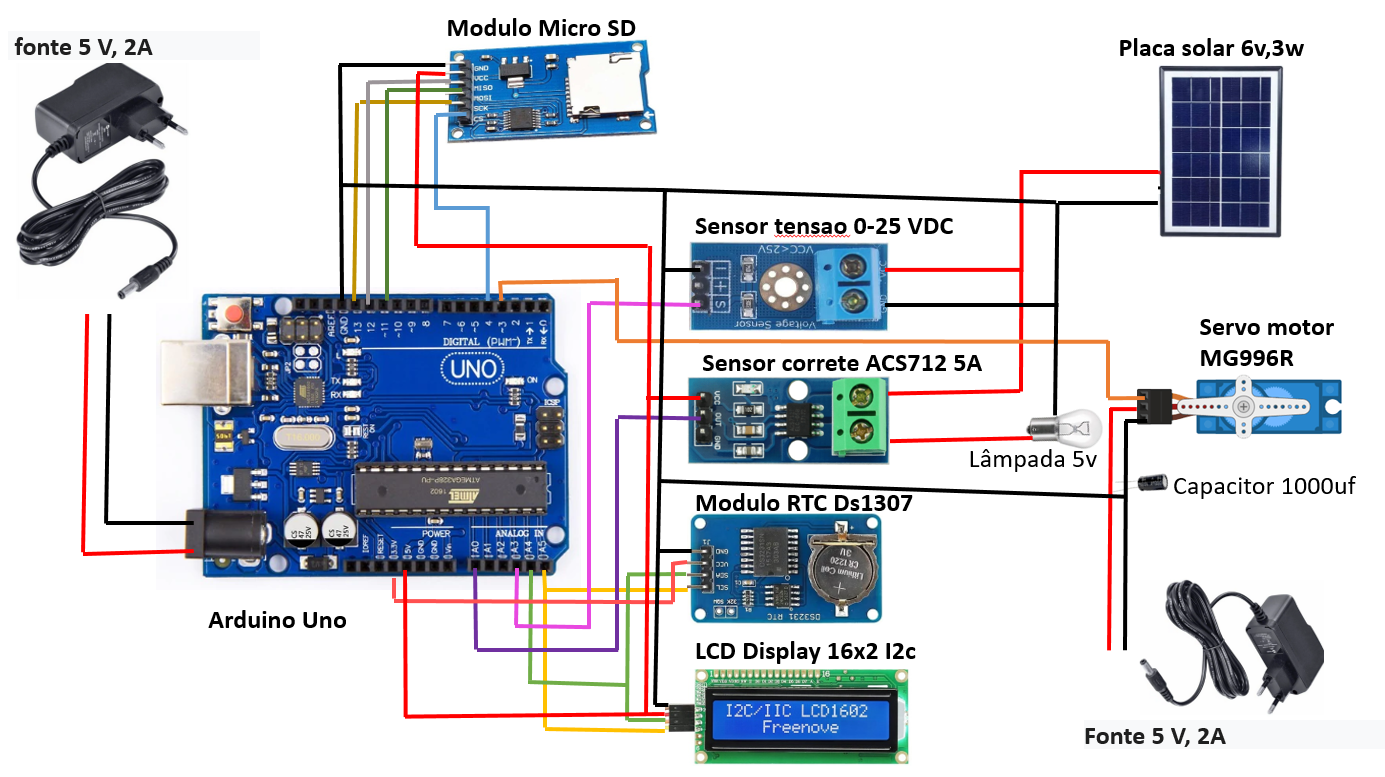
\includegraphics[width=0.9\textwidth]{Figuras/esquema.png}
    \caption{Esquema eletrônico do sistema automatizado}
    \caption*{Fonte: Autor (2026).}
    \label{fig:esquema}
\end{figure}

 Nesse contexto, o Arduino Uno atua como unidade central de controle, sendo alimentado por uma fonte externa de 5 V e 2 A conectada ao pino de alimentação apropriado da placa, o que garante o funcionamento do microcontrolador e dos periféricos a ele conectados, conferindo autonomia ao sistema.

O servo motor, responsável pela movimentação do painel fotovoltaico, possui alimentação independente de 5 V e 2 A, estratégia adotada para evitar sobrecarga no regulador de tensão do Arduino. O terminal positivo do servo é conectado à fonte externa de 5 V, enquanto o terminal negativo é ligado no polo negativo da fonte e paralelamente ao polo Ground (negativo do sistema - GND), o qual é comum a todos os componentes compartilhado com o Arduino. O sinal de controle é aplicado ao pino digital 3 da placa, que fornece um sinal PWM responsável pelo ajuste do ângulo de rotação. Adicionalmente, foi inserido um capacitor eletrolítico de 1000 µF / 16 V entre os terminais de alimentação do servo, com a finalidade de estabilizar a tensão e reduzir ruídos elétricos decorrentes da operação do motor.

O módulo RTC DS1307 é responsável pelo fornecimento de data e hora ao sistema. Sua alimentação é realizada pelo pino de 5 V do Arduino, com o terminal de terra conectado ao GND. A comunicação com o microcontrolador ocorre por meio do protocolo I2C, utilizando os pinos A5 (SCL) e A4 (SDA), o que permite a troca eficiente de dados temporais.

O módulo leitor de cartão microSD é alimentado pelo pino de 5 V do Arduino, com o terminal de terra conectado ao GND. A comunicação com o microcontrolador é realizada por meio do protocolo Serial Peripheral Interface (SPI), utilizando os pinos digitais 4 (CS), 13 (SCK), 12 (MISO) e 11 (MOSI), possibilitando a gravação e leitura de dados de forma confiável.

O display LCD 16x2 com interface I2C também é alimentado pelo pino de 5 V do Arduino, com conexão ao GND comum. Assim como o módulo RTC, utiliza o barramento I2C, compartilhando os pinos A5 (SCL) e A4 (SDA), o que reduz a quantidade de conexões físicas necessárias e simplifica a integração entre os dispositivos.

O sensor de corrente ACS712 é alimentado com 5 V e GND provenientes do Arduino, tendo seu pino de saída analógica conectado ao pino A0, permitindo a leitura da corrente elétrica por meio do conversor analógico-digital do microcontrolador. De forma análoga, o sensor de tensão possui sua saída conectada ao pino analógico A3, com o GND compartilhado com o restante do sistema, possibilitando a medição da tensão gerada pelo painel fotovoltaico.

As informações coletadas são organizadas na Tabela~\ref{tab:conexoes}, a qual apresenta as conexões entre os componentes do sistema e os respectivos pinos do Arduino. A estrutura é composta por duas colunas, sendo a primeira destinada à identificação dos componentes e a segunda à descrição de suas respectivas conexões elétricas e de comunicação.

\begin{table}[H]
\centering
\caption{Conexões entre os componentes do sistema}
\label{tab:conexoes}
\renewcommand{\arraystretch}{1.3}
\begin{tabular}{|p{4.5cm}|p{9cm}|}
\hline
\textbf{Componente} & \textbf{Conexões Arduino} \\
\hline

\textbf{Servo Motor (MG996R)} & 
Sinal → Pino 3 \newline
VCC → Fonte externa 5V \newline
GND → GND Arduino + Negativo Fonte \\
\hline

\textbf{RTC DS1307} & 
SDA → A4 \newline
SCL → A5 \newline
VCC → 5V \newline
GND → GND \\
\hline

\textbf{Display LCD 16x2 (I2C)} & 
SDA → A4 \newline
SCL → A5 \newline
VCC → 5V \newline
GND → GND \\
\hline

\textbf{Módulo Micro SD} & 
CS → Pino 4 \newline
SCK → Pino 13 \newline
MISO → Pino 12 \newline
MOSI → Pino 11 \newline
VCC → 5V \newline
GND → GND \\
\hline

\textbf{Sensor de Corrente (ACS712)} & 
OUT → A0 \newline
VCC → 5V \newline
GND → GND \\
\hline

\textbf{Sensor de Tensão} & 
OUT → A3 \newline
VCC → 5V \newline
GND → GND \\
\hline

\end{tabular}
\legend{Fonte: Autor (2026).}
\end{table}

Um aspecto fundamental do projeto é a utilização de um terra comum (GND) entre todos os componentes do sistema. Essa prática é essencial para garantir uma referência elétrica consistente, evitando erros de medição, ruídos e falhas de comunicação entre os dispositivos.

Para fins de validação experimental, foi implementado um segundo sistema fotovoltaico de referência, composto por um painel em posição fixa. Esse sistema foi desenvolvido de forma independente, com circuito próprio e aquisição de dados realizada em paralelo ao sistema automatizado. Os dados coletados por ambos os sistemas são armazenados separadamente, permitindo uma comparação direta e consistente entre as condições de operação.

A principal diferença entre os sistemas reside na presença do mecanismo de movimentação do painel solar, inexistente no sistema fixo. Dessa forma, torna-se possível avaliar quantitativamente o ganho de desempenho proporcionado pela automação do sistema, com base em parâmetros como potência instantânea, energia acumulada e eficiência relativa.

A adoção dessa abordagem experimental, baseada na operação de dois sistemas independentes sob condições equivalentes, aumenta a confiabilidade dos resultados obtidos, possibilitando a validação prática e a comparação consistente do desempenho do modelo proposto.


\chapter{Resultados}
 \label{cap5_resultados}

\section{Resultados da Simulação Computacional}

Com o objetivo de avaliar o comportamento do sistema fotovoltaico automatizado, foi realizada uma simulação computacional utilizando o ambiente MATLAB/Simulink. O modelo desenvolvido permitiu comparar o desempenho de um sistema automatizado, capaz de manter o painel orientado em direção à maior incidência da radiação solar, com um sistema fotovoltaico de painel fixo.

A simulação foi executada para um período correspondente a 12 horas de operação, representando o intervalo aproximado entre o nascer e o pôr do Sol, utilizando as condições descritas na metodologia. A Figura~\ref{fig:potencia_simulacao} apresenta as curvas de potência obtidas para os sistemas automatizado e de painel fixo durante o período de simulação.

\begin{figure}[H]
\centering
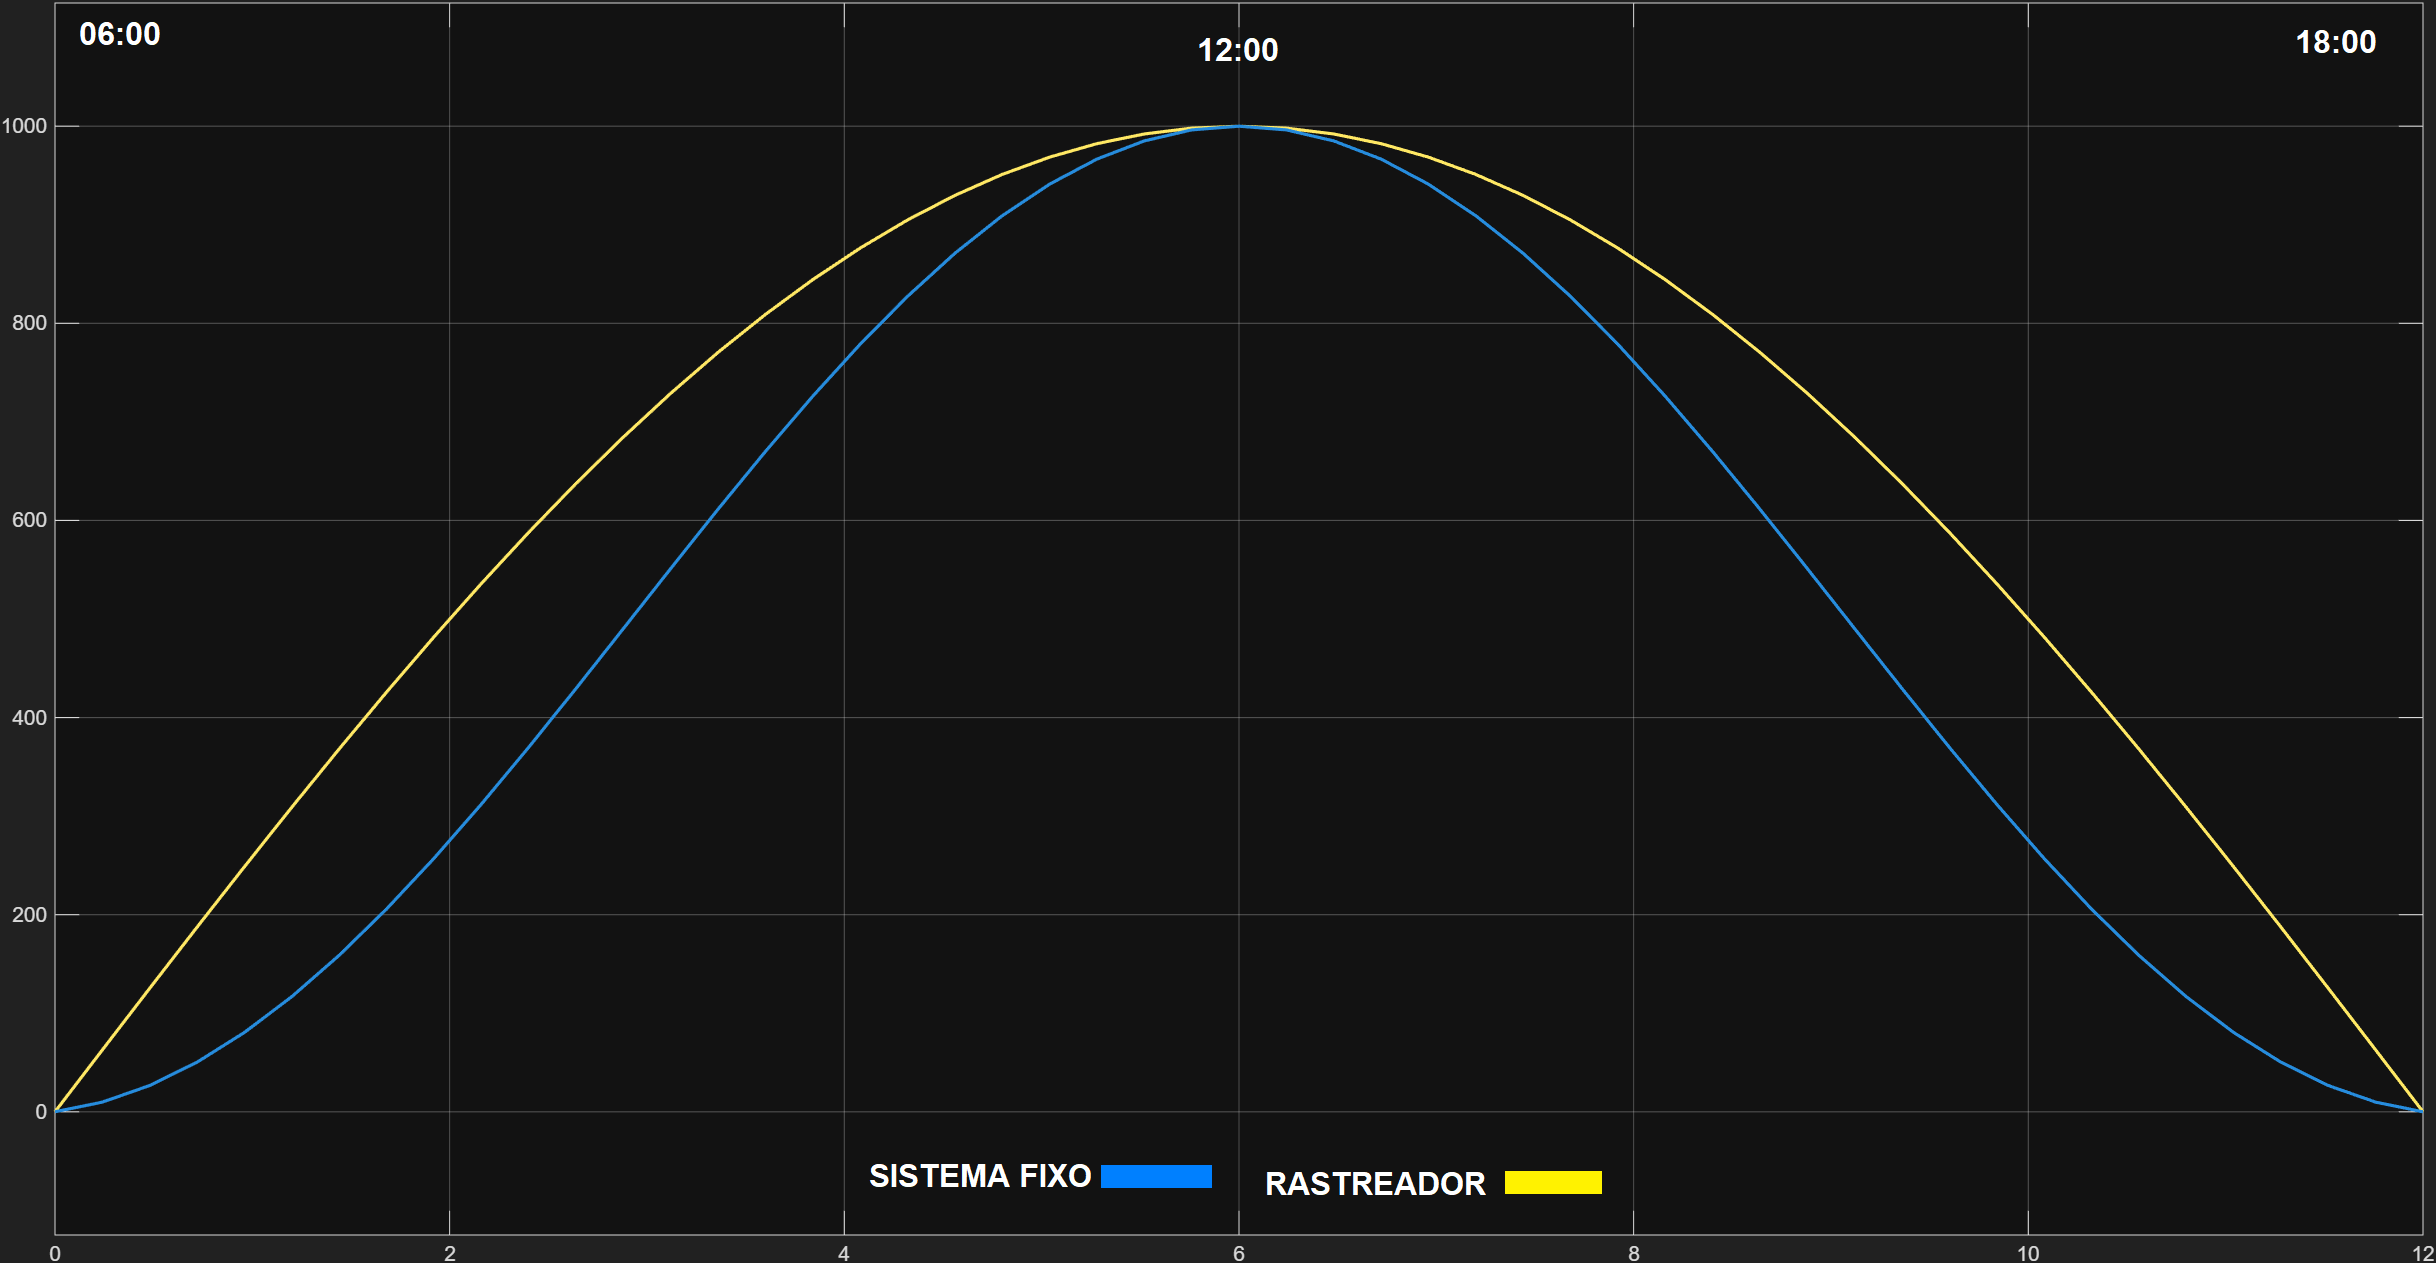
\includegraphics[width=0.85\textwidth]{Figuras/grafico_MS.png}
\caption{Curvas de potência obtidas na simulação computacional.}
\label{fig:potencia_simulacao}
\fonte{Autor (2026).}
\end{figure}

Observa-se que ambas as curvas acompanham a variação da irradiância ao longo do dia, apresentando aumento gradual da potência durante o período da manhã, valor máximo próximo ao meio-dia e redução ao longo da tarde. Entretanto, durante praticamente todo o período de simulação, o sistema automatizado apresentou valores de potência superiores aos do sistema de painel fixo.

Esse comportamento ocorre porque o modelo considera que o painel automatizado permanece continuamente orientado na direção de maior incidência da radiação solar, enquanto o painel fixo sofre perdas decorrentes da variação do ângulo de incidência da radiação ao longo do dia.

A integração das curvas de potência permitiu determinar a energia acumulada produzida por cada sistema durante todo o período de simulação. A partir desses valores foi calculado o ganho energético percentual do sistema automatizado em relação ao sistema de painel fixo.

Os resultados indicaram um ganho energético de aproximadamente \textbf{23,94\%}, evidenciando que o reposicionamento automatizado do painel proporciona maior aproveitamento da irradiância incidente e, consequentemente, maior geração de energia quando comparado ao sistema com painel fixo.

Embora o modelo utilize simplificações em relação às condições reais de operação, como irradiância idealizada e ausência de efeitos atmosféricos, os resultados obtidos apresentaram comportamento compatível com o esperado para sistemas fotovoltaicos com rastreamento solar de eixo único, fornecendo uma referência para a comparação com os dados experimentais obtidos pelo protótipo físico.

Na seção seguinte, os resultados da simulação são comparados aos dados experimentais, permitindo avaliar a capacidade do modelo computacional em representar o comportamento observado no sistema desenvolvido.

\section{Desempenho Experimental do Sistema}

Esta seção apresenta os resultados obtidos durante os ensaios experimentais realizados com o sistema fotovoltaico automatizado e com o sistema fotovoltaico de painel fixo. Conforme descrito na metodologia, ambos os sistemas operaram simultaneamente sob as mesmas condições ambientais, possibilitando a comparação direta de seus desempenhos ao longo do período experimental.

Os ensaios foram realizados entre os dias 23 e 26 de maio de 2026, com aquisição automática das variáveis elétricas entre 06h00 e 18h00, em intervalos de um minuto. A potência elétrica instantânea foi calculada a partir das medições de tensão e corrente registradas pelo sistema, conforme a Equação~\ref{eq:potencia}.

A energia produzida por cada sistema foi obtida pela integração numérica da potência ao longo do período de operação, permitindo determinar a produção energética diária de cada configuração. Com base nesses resultados, foi calculado o ganho percentual proporcionado pelo sistema automatizado em relação ao sistema de painel fixo.

Os resultados experimentais são apresentados inicialmente por meio das curvas de potência instantânea obtidas em cada dia de coleta. Em seguida, são analisados os valores de energia acumulada e o ganho energético proporcionado pelo sistema automatizado em comparação ao sistema de painel fixo. Por fim, os resultados experimentais são comparados aos obtidos pelo modelo computacional desenvolvido no MATLAB/Simulink, permitindo avaliar a representatividade da simulação em relação ao comportamento observado no protótipo físico.

\subsection{Curvas de Potência Instantânea}

As Figuras~\ref{fig:pot23}, \ref{fig:pot24}, \ref{fig:pot25} e~\ref{fig:pot26} apresentam as curvas de potência elétrica instantânea obtidas para o sistema automatizado e para o sistema com painel fixo durante os quatro dias de coleta experimental.

\begin{figure}[H]
\centering
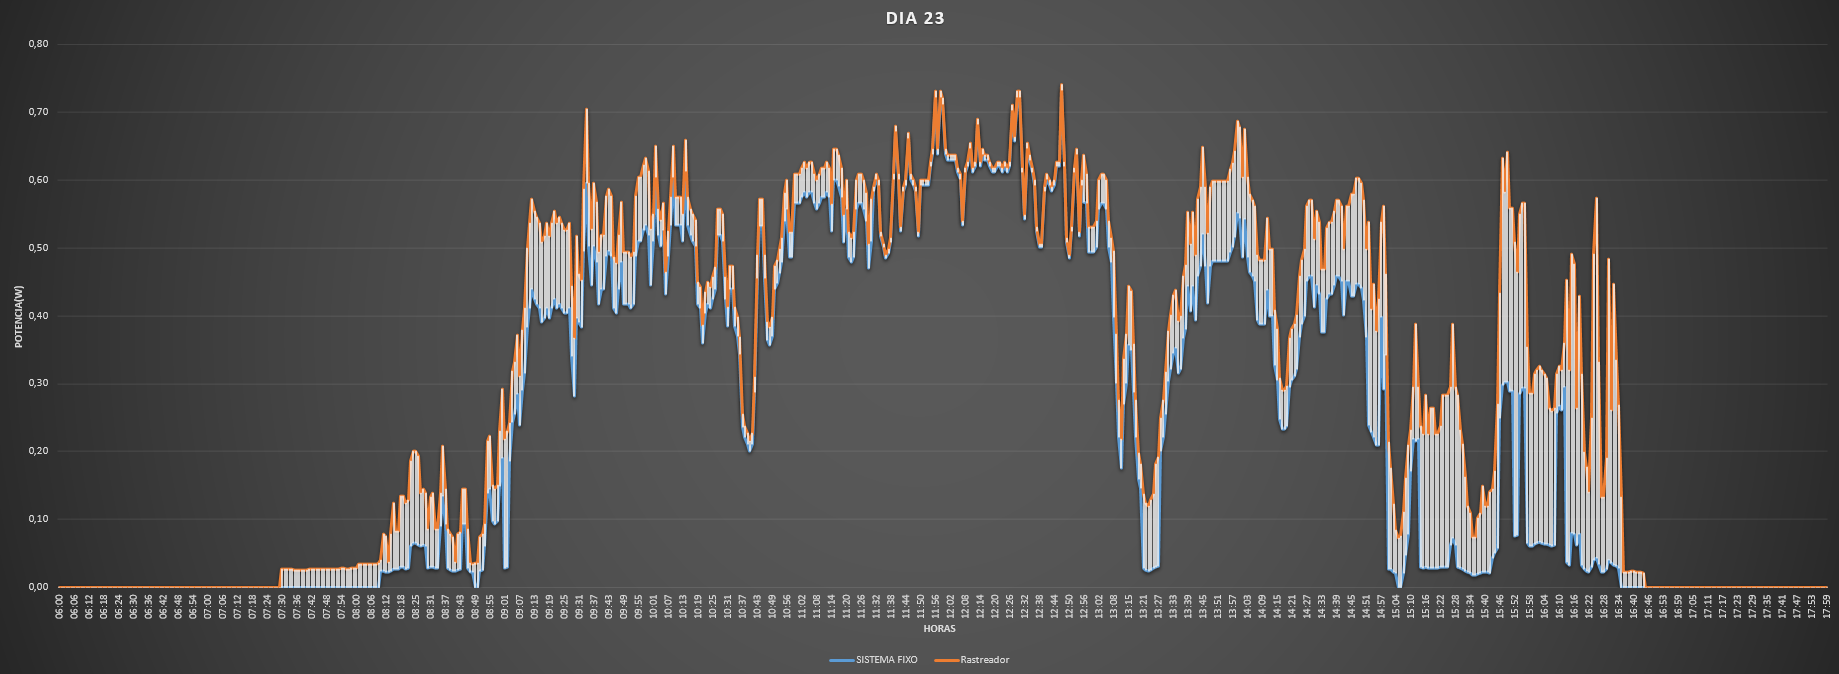
\includegraphics[width=0.90\textwidth]{Figuras/23_POTENCIA.png}
\caption{Curvas de potência dos sistemas automatizado e fixo em 23/05/2026.}
\label{fig:pot23}
\fonte{Autor (2026).}
\end{figure}

\begin{figure}[H]
\centering
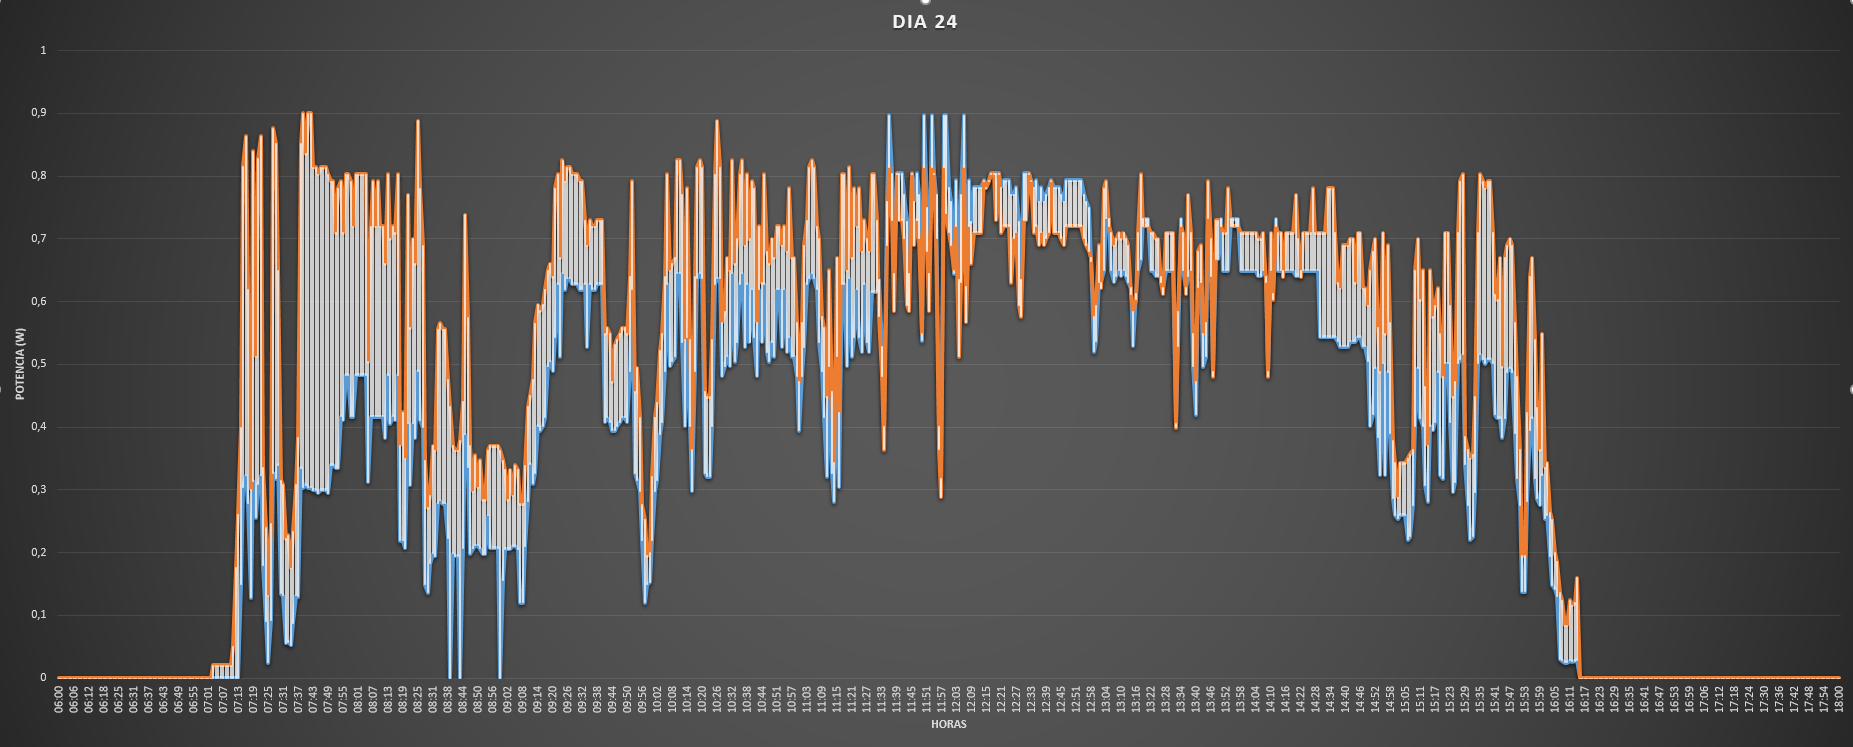
\includegraphics[width=0.90\textwidth]{Figuras/24_POTENCIA.png}
\caption{Curvas de potência dos sistemas automatizado e fixo em 24/05/2026.}
\label{fig:pot24}
\fonte{Autor (2026).}
\end{figure}

\begin{figure}[H]
\centering
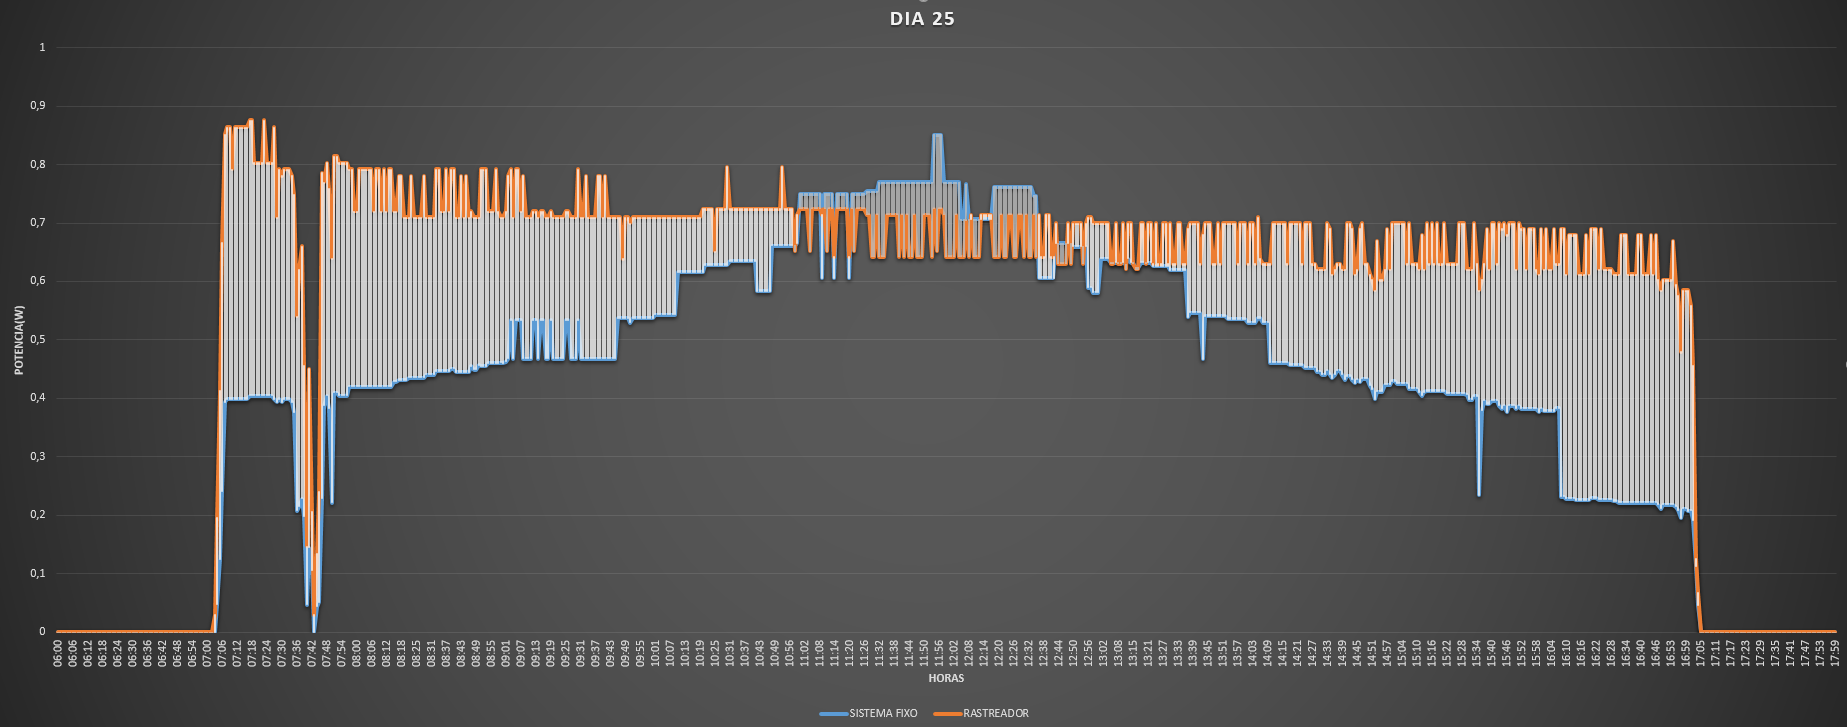
\includegraphics[width=0.90\textwidth]{Figuras/25_POTENCIA.png}
\caption{Curvas de potência dos sistemas automatizado e fixo em 25/05/2026.}
\label{fig:pot25}
\fonte{Autor (2026).}
\end{figure}

\begin{figure}[H]
\centering
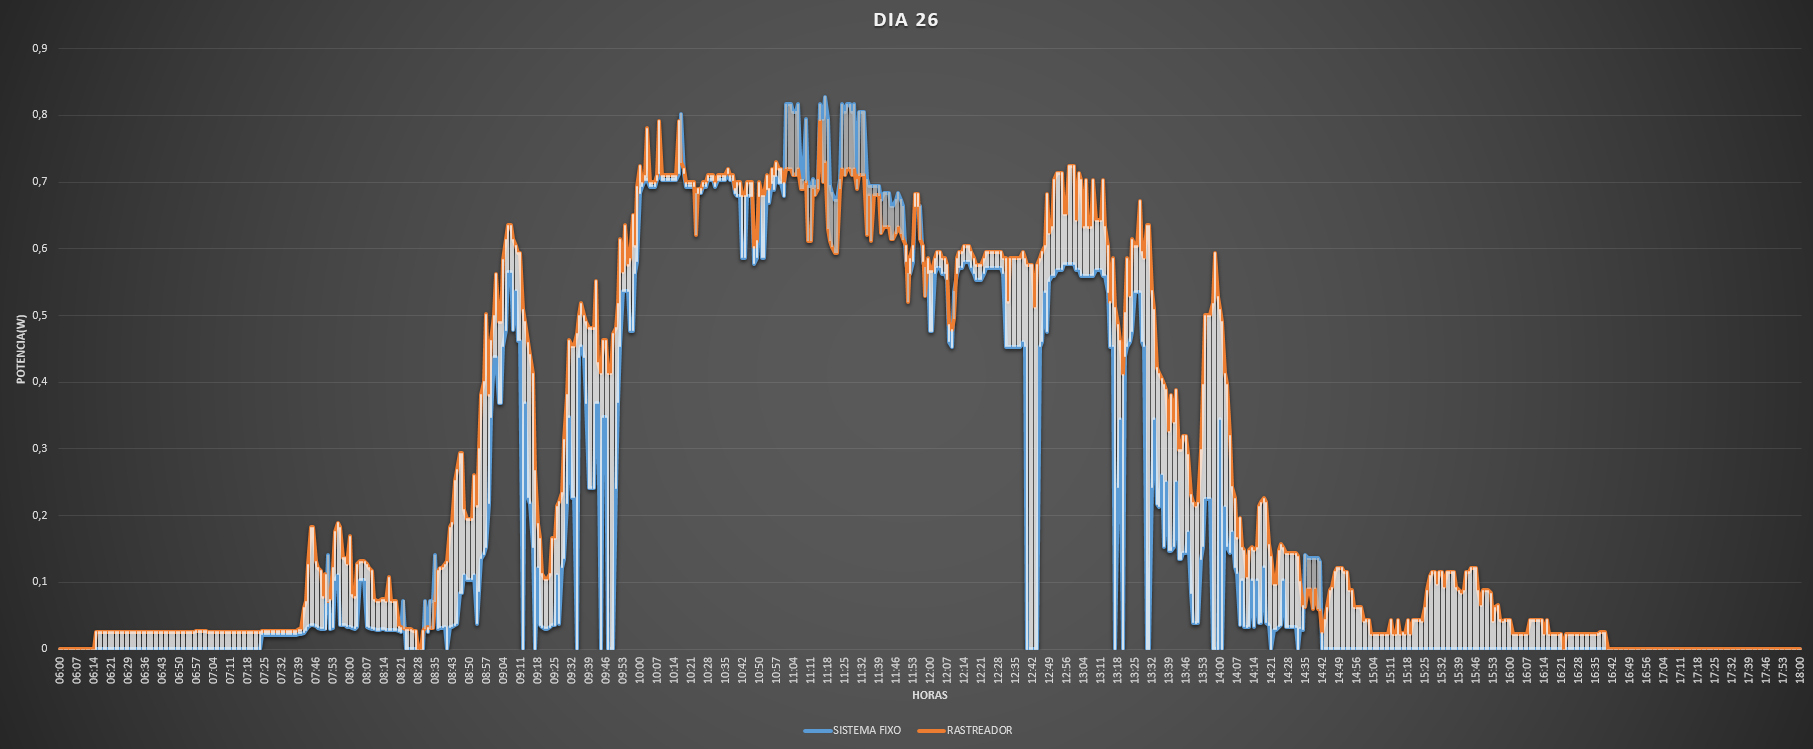
\includegraphics[width=0.90\textwidth]{Figuras/26_POTENCIA.png}
\caption{Curvas de potência dos sistemas automatizado e fixo em 26/05/2026.}
\label{fig:pot26}
\fonte{Autor (2026).}
\end{figure}

A análise conjunta das Figuras~\ref{fig:pot23} a~\ref{fig:pot26} evidencia um comportamento semelhante entre os quatro dias de ensaio. Em ambos os sistemas, a potência aumenta gradativamente após o nascer do Sol, atinge valores máximos próximos ao período de maior incidência da radiação solar e diminui progressivamente ao longo da tarde até o pôr do Sol.

Observa-se que o sistema automatizado apresentou valores de potência superiores aos do sistema com painel fixo durante a maior parte do período de operação. Esse comportamento está diretamente relacionado ao ajuste contínuo da orientação do painel fotovoltaico, reduzindo o ângulo de incidência da radiação solar sobre a superfície do módulo e aumentando o aproveitamento da irradiância disponível.

Embora ambos os sistemas tenham sido submetidos às mesmas condições ambientais, pequenas oscilações podem ser observadas nas curvas de potência ao longo do dia. Essas variações estão associadas principalmente à passagem de nuvens, alterações temporárias na irradiância solar, variações na temperatura das células fotovoltaicas e às incertezas inerentes ao processo de medição dos sensores utilizados.

Além dessas variações, observa-se que o sistema automatizado apresenta pequenas oscilações adicionais decorrentes da estratégia de controle implementada no algoritmo. Em intervalos regulares, o sistema realiza uma rotina de otimização local, efetuando pequenos deslocamentos angulares em torno da posição de referência e comparando a potência elétrica obtida em cada posição. Após essa comparação, o painel é reposicionado automaticamente no ângulo que proporciona a maior potência instantânea, o que resulta em pequenas variações nas curvas registradas.

Outro aspecto observado é que o ganho proporcionado pelo sistema automatizado torna-se mais evidente durante os períodos da manhã e da tarde. Nesses horários, o sistema com painel fixo apresenta maiores perdas decorrentes do aumento do ângulo de incidência da radiação solar, enquanto o sistema automatizado mantém o painel orientado de forma mais favorável. Próximo ao meio-dia, quando ambos os sistemas apresentam orientação semelhante em relação ao Sol, a diferença entre as potências tende a diminuir.

De maneira geral, os resultados experimentais demonstram que a estratégia de posicionamento adotada permitiu aumentar a potência instantânea produzida pelo módulo fotovoltaico ao longo do período de operação. Além de acompanhar o movimento aparente do Sol, o algoritmo realiza ajustes finos de posicionamento baseados na potência elétrica medida, buscando compensar pequenas diferenças entre a posição teórica e as condições reais de operação. Como consequência, observa-se um melhor aproveitamento da irradiância disponível quando comparado ao sistema convencional com painel fixo.

Embora as curvas de potência permitam analisar o comportamento instantâneo dos sistemas ao longo do dia, a comparação do desempenho energético é realizada de forma mais adequada por meio da energia acumulada produzida durante todo o período de operação. Os resultados dessa análise são apresentados na subseção seguinte.

\subsection{Valores Médios das Grandezas Elétricas}

Com o objetivo de avaliar o desempenho elétrico global dos sistemas ao longo do período experimental, foram calculados os valores médios de tensão, corrente e potência considerando todas as medições registradas durante os quatro dias de coleta. A Tabela~\ref{tab:medias_eletricas} apresenta os resultados obtidos para o sistema automatizado e para o sistema com painel fixo.

\begin{table}[H]
\centering
\caption{Valores médios das grandezas elétricas obtidos durante os ensaios experimentais.}
\label{tab:medias_eletricas}
\begin{tabular}{llccc}
\hline
\textbf{Grandeza} & \textbf{Sistema} & \textbf{Média} & \textbf{Unidade} & \textbf{Diferença (\%)}\\
\hline
Tensão  & Automatizado & 5,00 & V & \multirow{2}{*}{21,50}\\
         & Fixo         & 4,12 & V & \\
\hline
Corrente& Automatizado & 0,06 & A & \multirow{2}{*}{13,75}\\
         & Fixo         & 0,06 & A & \\
\hline
Potência& Automatizado & 0,41 & W & \multirow{2}{*}{29,39}\\
         & Fixo         & 0,31 & W & \\
\hline
\end{tabular}
\fonte{Autor (2026).}
\end{table}

Observa-se que o sistema automatizado apresentou valores médios superiores para todas as grandezas analisadas. Para a tensão elétrica, verificou-se um aumento médio de 21,50\% em relação ao sistema com painel fixo. De forma semelhante, a corrente elétrica apresentou aumento médio de 13,75\%. Embora as médias de corrente apresentadas na tabela sejam visualmente semelhantes devido ao arredondamento para duas casas decimais, o cálculo foi realizado utilizando os valores completos registrados durante os experimentos.

A maior diferença foi observada na potência elétrica, que apresentou aumento médio de 29,39\%. Esse resultado confirma que o reposicionamento automatizado do painel proporcionou melhor aproveitamento da radiação solar incidente, refletindo diretamente no aumento da potência produzida ao longo do período experimental.

As planilhas contendo todas as medições realizadas, bem como os valores médios obtidos para cada dia de experimento, encontram-se apresentadas no Apêndice~\ref{ap:apendiceC}. Adicionalmente, os arquivos utilizados no tratamento dos dados e nas análises desenvolvidas neste trabalho estão disponíveis no repositório descrito no Apêndice~\ref{ap:github}.

\subsection{Energia Acumulada e Ganho Energético}

Embora as curvas de potência permitam analisar o comportamento instantâneo dos sistemas, o parâmetro mais adequado para avaliar seu desempenho global é a energia elétrica produzida ao longo de todo o período de operação.

A energia diária foi determinada por meio da integração numérica da potência instantânea registrada durante o intervalo de coleta, compreendido entre 06h00 e 18h00. Como as medições foram realizadas em intervalos de um minuto, a energia produzida por cada sistema foi calculada conforme a Equação~\ref{eq:energia}.

\begin{equation}
E=\sum_{i=1}^{n}P_i\Delta t
\label{eq:energia}
\end{equation}

em que $E$ representa a energia acumulada (Wh), $P_i$ corresponde à potência instantânea medida em cada amostragem (W) e $\Delta t$ representa o intervalo entre as medições, equivalente a $1/60$ hora.

A Figura~\ref{fig:energia_Acumulada} apresenta a energia acumulada diariamente pelos sistemas automatizado e com painel fixo durante os quatro dias de monitoramento experimental.

\begin{figure}[H]
    \centering
    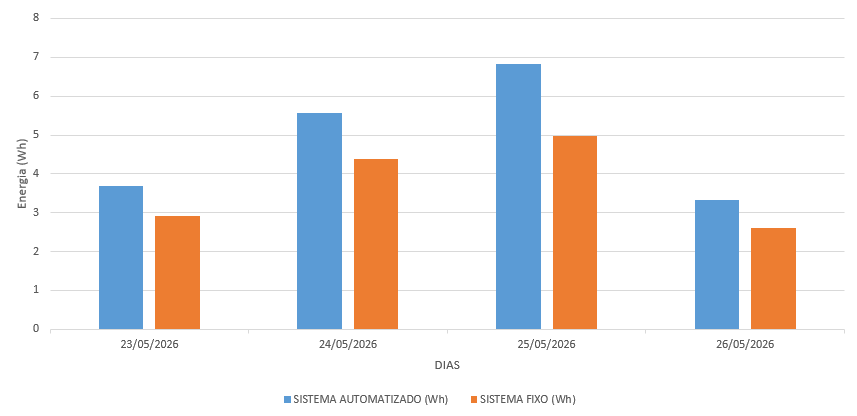
\includegraphics[width=0.85\textwidth]{Figuras/Energia_Acumulada.png}
    \caption{Energia acumulada diária dos sistemas fotovoltaicos automatizado e fixo.}
    \label{fig:energia_Acumulada}
    \fonte{Autor (2026).}
\end{figure}

Os valores numéricos da energia acumulada diária obtidos para cada sistema são apresentados na Tabela~\ref{tab:energia_diaria}.

\begin{table}[H]
\centering
\caption{Energia acumulada diária dos sistemas avaliados.}
\label{tab:energia_diaria}
\begin{tabular}{ccc}
\hline
Dia & Sistema automatizado (Wh) & Sistema fixo (Wh)\\
\hline
23/05/2026 & 3,70 & 2,92\\
24/05/2026 & 5,56 & 4,39\\
25/05/2026 & 6,82 & 4,98\\
26/05/2026 & 3,34 & 2,60\\
\hline
\end{tabular}
\fonte{Autor (2026).}
\end{table}

Para quantificar o desempenho do sistema automatizado em relação ao sistema com painel fixo, foi calculado o ganho energético percentual por meio da Equação~\ref{eq:ganho_energia}.

\begin{equation}
G(\%)=
\frac{E_{auto}-E_{fixo}}
{E_{fixo}}
\times100
\label{eq:ganho_energia}
\end{equation}

em que $E_{auto}$ representa a energia produzida pelo sistema automatizado e $E_{fixo}$ corresponde à energia produzida pelo sistema com painel fixo.

A análise da Figura~\ref{fig:energia_Acumulada} e da Tabela~\ref{tab:energia_diaria} mostra que o sistema automatizado apresentou maior produção de energia em todos os dias avaliados. O maior valor foi registrado em 25/05/2026, quando o sistema automatizado produziu aproximadamente 6,82 Wh, enquanto o sistema com painel fixo produziu 4,98 Wh. Nesse mesmo dia foi observado o maior ganho energético entre as duas configurações, de aproximadamente 36,95\%, indicando que, nas condições ambientais verificadas durante esse ensaio, o sistema automatizado obteve maior aproveitamento da irradiância incidente.

Os ganhos energéticos obtidos foram de 26,71\%, 26,65\%, 36,95\% e 28,46\% para os dias 23, 24, 25 e 26 de maio de 2026, respectivamente. Considerando todo o período experimental, o sistema automatizado acumulou aproximadamente 19,42 Wh, enquanto o sistema com painel fixo produziu cerca de 14,89 Wh, resultando em um ganho energético médio de aproximadamente 29,69\%.

Cabe destacar que os ganhos energéticos apresentados referem-se exclusivamente à energia elétrica produzida pelos módulos fotovoltaicos durante os ensaios experimentais. Não foi realizado o balanço energético considerando o consumo dos componentes utilizados no sistema automatizado, como o servomotor, o microcontrolador Arduino Uno, o display LCD, o módulo RTC, o cartão microSD e os sensores. Dessa forma, os valores obtidos representam o ganho da energia gerada pelo reposicionamento automático do painel, não correspondendo ao ganho líquido de energia do sistema completo. A avaliação do consumo energético do sistema de automação e sua influência sobre o ganho energético global constituem uma oportunidade para trabalhos futuros.

Esses resultados confirmam que o reposicionamento automático do painel proporcionou aumento consistente da energia produzida ao longo de todo o período experimental. Apesar das variações observadas entre os dias de coleta, decorrentes principalmente das condições ambientais, o sistema automatizado apresentou desempenho superior em todos os ensaios realizados, evidenciando a eficácia da estratégia de orientação adotada para maximizar o aproveitamento da radiação solar.
\chapter{Conclusão} 

\label{cap6_conclusao}

O presente trabalho teve como objetivo desenvolver um protótipo experimental de um sistema fotovoltaico automatizado de baixo custo para avaliar a influência do reposicionamento automático do painel fotovoltaico na geração de energia elétrica, bem como desenvolver e validar um modelo computacional no ambiente MATLAB/Simulink por meio da comparação entre resultados simulados e experimentais.

Os resultados experimentais demonstraram que o sistema automatizado apresentou desempenho superior ao sistema com painel fixo durante todo o período de monitoramento. A análise das curvas de potência e da energia acumulada evidenciou que o reposicionamento automático do painel proporcionou um ganho energético médio de aproximadamente 29,69\%, confirmando que a estratégia de orientação adotada aumenta o aproveitamento da radiação solar incidente quando comparada à utilização de um painel mantido em posição fixa.

Na simulação computacional, o modelo desenvolvido no MATLAB/Simulink indicou um ganho energético de aproximadamente 23,94\% para o sistema automatizado em relação ao sistema com painel fixo. Embora esse valor seja inferior ao obtido experimentalmente, ambos apresentam a mesma tendência de aumento da geração de energia proporcionada pelo reposicionamento automático do painel. A proximidade entre os resultados simulados e experimentais demonstra que o modelo foi capaz de representar satisfatoriamente o comportamento geral do sistema, atendendo ao objetivo de validação proposto neste trabalho.

O protótipo desenvolvido cumpriu sua finalidade como plataforma experimental para aquisição de dados e validação do modelo computacional. A integração entre Arduino Uno, sensores de tensão e corrente, servomotor, módulo RTC, display LCD e cartão microSD possibilitou a implementação de um sistema capaz de realizar automaticamente o monitoramento das variáveis elétricas, o controle do posicionamento do painel fotovoltaico e o armazenamento dos dados experimentais.

Entretanto, os resultados devem ser analisados considerando as limitações inerentes à pesquisa. O protótipo foi desenvolvido exclusivamente para fins experimentais, utilizando um módulo fotovoltaico de pequena potência e uma estrutura mecânica simplificada, não representando uma solução destinada à aplicação em sistemas fotovoltaicos comerciais. Além disso, não foram avaliados aspectos relacionados à durabilidade mecânica da estrutura, aos custos de implantação e manutenção, ao consumo energético dos componentes eletrônicos utilizados na automação e à viabilidade técnico-econômica da solução proposta. Os ganhos energéticos apresentados referem-se exclusivamente ao aumento da energia produzida pelo painel fotovoltaico em decorrência do reposicionamento automático, não considerando o consumo dos dispositivos responsáveis pela automação do sistema. Também não foram incorporadas ao modelo computacional medições reais de irradiância e temperatura durante os ensaios experimentais, uma vez que o objetivo do estudo concentrou-se na análise do ganho de energia proporcionado pelo reposicionamento automático do painel.

Apesar dessas limitações, os resultados obtidos fornecem evidências experimentais de que a orientação automática do painel fotovoltaico contribui para o aumento da energia gerada ao longo do dia. Além disso, demonstram que o modelo computacional desenvolvido representa adequadamente o comportamento observado no protótipo físico, podendo ser utilizado como ferramenta de apoio em análises e estudos comparativos de sistemas fotovoltaicos automatizados.

Conclui-se, portanto, que os objetivos propostos foram plenamente alcançados. Foi possível desenvolver o protótipo experimental, implementar o sistema de aquisição e controle, construir e validar o modelo computacional e comparar os resultados simulados com os dados obtidos em condições reais de operação. Os resultados evidenciam que a utilização de sistemas embarcados associados a técnicas de automação constitui uma alternativa tecnicamente viável para aumentar o aproveitamento da energia solar em aplicações experimentais. Assim, este trabalho contribui para o desenvolvimento de pesquisas relacionadas a sistemas fotovoltaicos automatizados, modelagem computacional, geração distribuída e energias renováveis, fornecendo uma base experimental que poderá ser utilizada em estudos futuros voltados ao aperfeiçoamento de sistemas de rastreamento solar e à avaliação de sua viabilidade em aplicações de maior escala.

%-----------------------------------
% Finaliza a parte no bookmark do PDF
% para que se inicie o bookmark na raiz
% e adiciona espaço de parte no Sumário
\phantompart

%-----------------------------------
% Bibliografia
\bibliography{referencias.bib}


%-----------------------------------
% POST-TEXTUAL ELEMENTS
%-----------------------------------
\postextual

% Anexos
% Elemento opcional
%-----------------------------------
%\begin{anexosenv}
%\partanexos

% ANEXO A – Servo Motor
%\includepdf[
%pages=1,
%scale=0.75,
%pagecommand={\chapter{\texorpdfstring{Datasheet do Servo Motor MG996R}{Datasheet do Servo Motor MG996R}}}
%]{pos-textuais/MG996R.PDF}

%\includepdf[
%pages=2,
%scale=0.90,
%pagecommand={}
%]{pos-textuais/MG996R.PDF}

% ANEXO B – RTC DS1307
%\includepdf[
%pages=1,
%scale=0.75,
%pagecommand={\chapter{Datasheet do Módulo RTC DS1307}}
%]{pos-textuais/DS1307.pdf}

%\includepdf[
%pages=2,
%scale=0.90,
%pagecommand={}
%]{pos-textuais/DS1307.pdf}

% ANEXO C – ACS712
%\includepdf[
%pages=1,
%scale=0.75,
%pagecommand={\chapter{Datasheet do Sensor ACS712}}
%]{pos-textuais/acs712.pdf}

%\includepdf[
%pages=2,
%scale=0.80,
%pagecommand={}
%]{pos-textuais/acs712.pdf}

% ANEXO D – Display LCD I2C
%\includepdf[
%pages=1,
%scale=0.65,
%pagecommand={\chapter{Datasheet do Display LCD com Interface I2C}}
%]{pos-textuais/I2C_1602_LCD.pdf}

%\includepdf[
%pages=2,
%scale=0.90,
%pagecommand={}
%]{pos-textuais/I2C_1602_LCD.pdf}

% ANEXO E – Módulo SD
%\includepdf[
%pages=1,
%scale=0.80,
%pagecommand={\chapter{Datasheet do Módulo Leitor de Cartão SD}}
%]{pos-textuais/MicroSD-Module.pdf}

%\includepdf[
%pages=2,
%scale=0.90,
%pagecommand={}
%]{pos-textuais/MicroSD-Module.pdf}

%\end{anexosenv}

% Apêndice
% Elemento opcional
%-----------------------------------
%====================================================
% APÊNDICES
% Material elaborado pelo autor
%====================================================

\begin{apendicesenv}

\partapendices

\chapter{Código-Fonte do Sistema Embarcado em Arduino}

Neste apêndice, apresenta-se o código-fonte desenvolvido para o controle do sistema automatizado. O algoritmo contempla as rotinas de leitura dos sensores, acionamento do servo motor, registro de dados e exibição das informações em display LCD. Com o objetivo de facilitar a compreensão, o código foi integralmente comentado, descrevendo detalhadamente o funcionamento de cada etapa do sistema.

% \input{pos-textuais/codigo_arduino.tex}
\begin{verbatim}



 
// Sistema com Otimização 


#include <Wire.h>
#include <RTClib.h>
#include <Servo.h>
#include <LiquidCrystal_I2C.h>
#include <SPI.h>
#include <SD.h>

RTC_DS1307 rtc;
Servo servoMotor;
LiquidCrystal_I2C lcd(0x27,16,2);
File dataFile;

#define SERVO_PIN   3
#define VOLT_PIN    A3
#define ACS712_PIN  A0
#define SD_CS       4

char nomeTXT[] = "LOG.TXT";

float anguloAtual = 90;
float anguloAlvo  = 90;

unsigned long tempoAnterior   = 0;
unsigned long tempoGravacao   = 0;
unsigned long tempoOtimizacao = 0;

int tela = 0;

float tensaoFiltrada  = 0;
float correnteFiltrada = 0;

int anguloInicio = 25;
int anguloMeio   = 90;
int anguloFim    = 150;


// FUNÇÃO: calcularAngulo()
// Calcula o ângulo teórico do painel conforme o horário atual.

float calcularAngulo(DateTime now)
{
    int minutosAtual = now.hour()*60 + now.minute();

    int inicio = 6*60;
    int meio   = 12*60;
    int fim    = 18*60;

    if(minutosAtual < inicio)
        return anguloInicio;

    if(minutosAtual <= meio)
    {
        float p = (float)(minutosAtual-inicio)/(meio-inicio);
        return anguloInicio + p*(anguloMeio-anguloInicio);
    }

    if(minutosAtual <= fim)
    {
        float p = (float)(minutosAtual-meio)/(fim-meio);
        return anguloMeio + p*(anguloFim-anguloMeio);
    }

    return anguloInicio;
}


// FUNÇÃO: atualizarServo()
// Realiza deslocamento gradual para evitar movimentos bruscos.

void atualizarServo()
{
    float diferenca = anguloAlvo - anguloAtual;

    if(abs(diferenca) > 0.2)
    {
        float passo = diferenca * 0.03;

        if(passo > 1) passo = 1;
        if(passo < -1) passo = -1;

        anguloAtual += passo;
        servoMotor.write((int)anguloAtual);
    }
}


 //  FUNÇÃO: lerTensao()

float lerTensao()
{
    long soma = 0;

    for(int i=0;i<10;i++)
    {
        soma += analogRead(VOLT_PIN);
        delay(2);
    }

    float media = soma/10.0;

    return media*(5.0/1023.0)*5.0;
}


 // FUNÇÃO: lerCorrente()

float lerCorrente()
{
    long soma = 0;

    for(int i=0;i<20;i++)
    {
        soma += analogRead(ACS712_PIN);
        delay(2);
    }

    float media = soma/20.0;

    float corrente =
        (media - 512) *
        (5.0/1023.0) /
        0.185;

    if(corrente < 0)
        corrente = 0;

    return corrente;
}


// FUNÇÃO: medirPotencia()

float medirPotencia()
{
    return lerTensao() * lerCorrente();
}


// FUNÇÃO: otimizarAngulo()
// Busca o melhor ângulo baseado na potência gerada.

float otimizarAngulo(float anguloBase)
{
    float melhorAngulo = anguloBase;
    float melhorPotencia = 0;

    for(int ajuste=-10; ajuste<=10; ajuste+=3)
    {
        float anguloTeste = anguloBase + ajuste;

        if(anguloTeste < 0) anguloTeste = 0;
        if(anguloTeste > 180) anguloTeste = 180;

        servoMotor.write((int)anguloTeste);

        delay(300);

        float potencia = medirPotencia();

        if(potencia > melhorPotencia)
        {
            melhorPotencia = potencia;
            melhorAngulo = anguloTeste;
        }
    }

    return melhorAngulo;
}


// FUNÇÃO: salvarSD()
// Registra data, hora, tensão, corrente, potência e ângulo.

void salvarSD(DateTime now,float V,float I,float P,float A)
{
    dataFile = SD.open(nomeTXT, FILE_WRITE);

    if(dataFile)
    {
        dataFile.print(now.day());
        dataFile.print('/');
        dataFile.print(now.month());
        dataFile.print('/');
        dataFile.print(now.year());
        dataFile.print(' ');

        dataFile.print(now.hour());
        dataFile.print(':');
        dataFile.print(now.minute());

        dataFile.print(" V=");
        dataFile.print(V,1);

        dataFile.print(" I=");
        dataFile.print(I,2);

        dataFile.print(" P=");
        dataFile.print(P,1);

        dataFile.print(" A=");
        dataFile.println((int)A);

        dataFile.close();
    }
}

void setup()
{
    Serial.begin(9600);

    Wire.begin();
    rtc.begin();

    lcd.init();
    lcd.backlight();

    servoMotor.attach(SERVO_PIN);

    DateTime now = rtc.now();

    anguloAtual = calcularAngulo(now);
    anguloAlvo  = anguloAtual;

    servoMotor.write((int)anguloAtual);

    if(!SD.begin(SD_CS))
    {
        lcd.print("Erro SD");
        while(1);
    }

    lcd.print("Sistema OK");
    delay(1500);
    lcd.clear();
}

void loop()
{
    DateTime now = rtc.now();

    float anguloBase = calcularAngulo(now);

// tempo para fazer verificaçao de melhor angulo a cada 10 minutos

    if(millis()-tempoOtimizacao >= 600000) 
    {
        tempoOtimizacao = millis();
        anguloAlvo = otimizarAngulo(anguloBase);
    }

    atualizarServo();

    float tensao = lerTensao();
    float corrente = lerCorrente();

    tensaoFiltrada =
        tensaoFiltrada*0.9 +
        tensao*0.1;

    correnteFiltrada =
        correnteFiltrada*0.9 +
        corrente*0.1;

    float potencia =
        tensaoFiltrada *
        correnteFiltrada;

    if(now.hour() >= 6 && now.hour() < 18)
    {
        if(millis()-tempoGravacao >= 60000)
        {
            tempoGravacao = millis();

            salvarSD(
                now,
                tensaoFiltrada,
                correnteFiltrada,
                potencia,
                anguloAtual
            );
        }
    }

    if(millis()-tempoAnterior > 3000)
    {
        tela++;

        if(tela > 1)
            tela = 0;

        tempoAnterior = millis();

        lcd.clear();
    }

    if(tela == 0)
    {
        lcd.setCursor(0,0);
        lcd.print(now.day());
        lcd.print('/');
        lcd.print(now.month());
        lcd.print(' ');
        lcd.print(now.hour());
        lcd.print(':');
        lcd.print(now.minute());

        lcd.setCursor(0,1);
        lcd.print("ANG:");
        lcd.print((int)anguloAtual);
    }

    if(tela == 1)
    {
        lcd.setCursor(0,0);
        lcd.print("V=");
        lcd.print(tensaoFiltrada,1);

        lcd.print(" I=");
        lcd.print(correnteFiltrada,2);

        lcd.setCursor(0,1);
        lcd.print("P=");
        lcd.print(potencia,1);
    }

    delay(200);
}



\end{verbatim}

\chapter{Script de Simulação Desenvolvido no MATLAB}

Neste apêndice é apresentado o script utilizado para a geração automática do modelo computacional no ambiente \textit{MATLAB/Simulink}, empregado na comparação entre um sistema fotovoltaico fixo e um sistema com automação. O código foi estruturado e comentado com o objetivo de facilitar a compreensão de todas as etapas da modelagem, incluindo a criação dos blocos, a definição dos parâmetros, o estabelecimento das conexões e a configuração da simulação.

O modelo computacional foi desenvolvido com base na metodologia proposta por Farrukh Nagi, apresentada no trabalho Fixed vs Tracking Solar Panel Output Comparison in Simulink, disponibilizado na plataforma MATLAB Central File Exchange em 2023. A proposta original consiste na comparação do desempenho de sistemas fotovoltaicos fixos e sistemas com automação por meio de uma modelagem realizada no ambiente Simulink.

Para atender aos objetivos desta pesquisa, o modelo de referência foi adaptado e expandido, incorporando funcionalidades adicionais, tais como o cálculo da energia acumulada ao longo da simulação, a determinação do ganho percentual instantâneo e a avaliação do ganho energético total proporcionado pelo sistema automatizado. Além disso, foram realizadas melhorias na organização estrutural e na documentação do código, visando aumentar sua clareza, e adequação às análises desenvolvidas neste trabalho.

A referência utilizada como base para o desenvolvimento do modelo é apresentada a seguir:

NAGI, Farrukh. Fixed vs Tracking Solar Panel Output Comparison in Simulink. MATLAB Central File Exchange, 2023.

Disponível em: https://www.mathworks.com/matlabcentral/fileexchange/123655-fixed-vs-tracking-solar-panel-output-comparison-in-simulink. Acesso em: 02 março 2026.

O código original encontra-se disponibilizado sob licença BSD 3-Clause.




\begin{verbatim}

%% 

clc;
clear;
close all;

%% 
% CRIAÇÃO DO MODELO
%% 
modelName = 'Sistema Automatizado';

if bdIsLoaded(modelName)
    close_system(modelName,0);
end

new_system(modelName);
open_system(modelName);

%% 
% CONFIGURAÇÃO VISUAL
%% 
x  = 50;
y  = 100;
dx = 130;

%% 
%% 
%
% O bloco Clock fornece continuamente o tempo da simulação.
%
% O ganho pi/12 converte o tempo em radianos para utilização
% na função seno que representa a trajetória solar.
%

add_block('simulink/Sources/Clock', ...
    [modelName '/Tempo'], ...
    'Position',[x y x+40 y+30]);

add_block('simulink/Math Operations/Gain', ...
    [modelName '/Graus'], ...
    'Gain','pi/12', ...
    'Position',[x+dx y x+dx+40 y+30]);

%% 
%  TRAJETÓRIA SOLAR
%% 
%
% A posição aparente do Sol é representada por:
%
% f(t) = sen(pi*t/12)
%
% t = 0 h  -> nascer do Sol
% t = 6 h  -> máxima incidência
% t = 12 h -> pôr do Sol
%

add_block('simulink/Math Operations/Trigonometric Function', ...
    [modelName '/Trajetoria_Sol'], ...
    'Operator','sin', ...
    'Position',[x+2*dx y x+2*dx+40 y+30]);

%% 
%  COMPONENTES DA IRRADIÂNCIA
%% 
%
% Irradiância Direta = 900 W/m²
% Irradiância Difusa = 100 W/m²
%
% Valor máximo total:
%
% 1000 W/m²
%
% Compatível com condições padrão de teste (STC).
%

add_block('simulink/Math Operations/Gain', ...
    [modelName '/Luz_Difusa'], ...
    'Gain','100', ...
    'Position',[x+3*dx y-50 x+3*dx+40 y-20]);

add_block('simulink/Math Operations/Gain', ...
    [modelName '/Luz_Direta'], ...
    'Gain','900', ...
    'Position',[x+3*dx y+30 x+3*dx+40 y+60]);

%% 
%  SISTEMA FIXO
%% 
%
% O sistema fixo sofre perdas associadas ao desalinhamento angular.
%
% O fator angular reduz a parcela de irradiância direta recebida
% pelo módulo fotovoltaico.
%

add_block('simulink/Math Operations/Product', ...
    [modelName '/Fator_Angulo'], ...
    'Inputs','2', ...
    'Position',[x+4*dx y+70 x+4*dx+40 y+110]);

%% 
%  POTÊNCIA DOS SISTEMAS
%% 
%
% Tracker:
% Potência = Direta + Difusa
%
% Fixo:
% Potência = Difusa + (Direta × Fator Angular)
%

add_block('simulink/Math Operations/Add', ...
    [modelName '/Potencia_Tracker'], ...
    'Inputs','++', ...
    'Position',[x+5*dx y-30 x+5*dx+40 y+10]);

add_block('simulink/Math Operations/Add', ...
    [modelName '/Potencia_Fixo'], ...
    'Inputs','++', ...
    'Position',[x+5*dx y+50 x+5*dx+40 y+90]);

%% 
%  GANHO INSTANTÂNEO (%)
%% 

add_block('simulink/Math Operations/Subtract', ...
    [modelName '/Diferenca'], ...
    'Position',[x+6*dx y+100 x+6*dx+40 y+130]);

add_block('simulink/Sources/Constant', ...
    [modelName '/Epsilon'], ...
    'Value','0.01', ...
    'Position',[x+6*dx y+150 x+6*dx+40 y+180]);

add_block('simulink/Math Operations/Add', ...
    [modelName '/Fixo_Seguro'], ...
    'Inputs','++', ...
    'Position',[x+7*dx y+120 x+7*dx+40 y+150]);

add_block('simulink/Math Operations/Divide', ...
    [modelName '/Divisao'], ...
    'Position',[x+8*dx y+100 x+8*dx+40 y+130]);

add_block('simulink/Math Operations/Gain', ...
    [modelName '/Ganho_Percentual'], ...
    'Gain','100', ...
    'Position',[x+9*dx y+100 x+9*dx+40 y+130]);

%% 
%  ENERGIA ACUMULADA
%% 
%
% Energia =  Potência dt
%

add_block('simulink/Continuous/Integrator', ...
    [modelName '/Energia_Tracker'], ...
    'Position',[x+6*dx y-30 x+6*dx+40 y]);

add_block('simulink/Continuous/Integrator', ...
    [modelName '/Energia_Fixo'], ...
    'Position',[x+6*dx y+50 x+6*dx+40 y+80]);

%% 
%  GANHO ENERGÉTICO TOTAL (%)
%% 

add_block('simulink/Math Operations/Subtract', ...
    [modelName '/Dif_Energia'], ...
    'Position',[x+8*dx y+20 x+8*dx+40 y+50]);

add_block('simulink/Sources/Constant', ...
    [modelName '/Epsilon_Energia'], ...
    'Value','0.01', ...
    'Position',[x+8*dx y+70 x+8*dx+40 y+100]);

add_block('simulink/Math Operations/Add', ...
    [modelName '/Energia_Fixo_Seguro'], ...
    'Inputs','++', ...
    'Position',[x+9*dx y+50 x+9*dx+40 y+80]);

add_block('simulink/Math Operations/Divide', ...
    [modelName '/Div_Energia'], ...
    'Position',[x+10*dx y+20 x+10*dx+40 y+50]);

add_block('simulink/Math Operations/Gain', ...
    [modelName '/Ganho_Total_Percentual'], ...
    'Gain','100', ...
    'Position',[x+11*dx y+20 x+11*dx+40 y+50]);

%% 
%  VISUALIZAÇÃO
%% 
%
% O Scope exibirá apenas:
%
% • Sistema Automatizado
% • Sistema Fixo
%

add_block('simulink/Signal Routing/Mux', ...
    [modelName '/Mux'], ...
    'Inputs','2', ...
    'Position',[x+9*dx y x+9*dx+10 y+60]);

add_block('simulink/Sinks/Scope', ...
    [modelName '/Grafico_Linha'], ...
    'Position',[x+10*dx y x+10*dx+60 y+70]);

add_block('simulink/Sinks/Display', ...
    [modelName '/Display_Ganho_Final'], ...
    'Position',[x+12*dx y+20 x+12*dx+80 y+60]);

%% 
% CONEXÕES
%% 

add_line(modelName,'Tempo/1','Graus/1');
add_line(modelName,'Graus/1','Trajetoria_Sol/1');

add_line(modelName,'Trajetoria_Sol/1','Luz_Difusa/1');
add_line(modelName,'Trajetoria_Sol/1','Luz_Direta/1');

add_line(modelName,'Luz_Difusa/1','Potencia_Tracker/1');
add_line(modelName,'Luz_Direta/1','Potencia_Tracker/2');

add_line(modelName,'Trajetoria_Sol/1','Fator_Angulo/2');
add_line(modelName,'Luz_Direta/1','Fator_Angulo/1');

add_line(modelName,'Luz_Difusa/1','Potencia_Fixo/1');
add_line(modelName,'Fator_Angulo/1','Potencia_Fixo/2');

add_line(modelName,'Potencia_Tracker/1','Diferenca/1');
add_line(modelName,'Potencia_Fixo/1','Diferenca/2');

add_line(modelName,'Potencia_Fixo/1','Fixo_Seguro/1');
add_line(modelName,'Epsilon/1','Fixo_Seguro/2');

add_line(modelName,'Diferenca/1','Divisao/1');
add_line(modelName,'Fixo_Seguro/1','Divisao/2');

add_line(modelName,'Divisao/1','Ganho_Percentual/1');

add_line(modelName,'Potencia_Tracker/1','Energia_Tracker/1');
add_line(modelName,'Potencia_Fixo/1','Energia_Fixo/1');

add_line(modelName,'Energia_Tracker/1','Dif_Energia/1');
add_line(modelName,'Energia_Fixo/1','Dif_Energia/2');

add_line(modelName,'Energia_Fixo/1','Energia_Fixo_Seguro/1');
add_line(modelName,'Epsilon_Energia/1','Energia_Fixo_Seguro/2');

add_line(modelName,'Dif_Energia/1','Div_Energia/1');
add_line(modelName,'Energia_Fixo_Seguro/1','Div_Energia/2');

add_line(modelName,'Div_Energia/1','Ganho_Total_Percentual/1');

add_line(modelName,'Ganho_Total_Percentual/1','Display_Ganho_Final/1');

% Scope (somente dois sinais)
add_line(modelName,'Potencia_Tracker/1','Mux/1');
add_line(modelName,'Potencia_Fixo/1','Mux/2');

add_line(modelName,'Mux/1','Grafico_Linha/1');

%% 
% CONFIGURAÇÃO FINAL
%% 

set_param(modelName,'StopTime','12');

save_system(modelName);

disp('fim');


\end{verbatim}


\chapter{Planilhas de Coleta de Dados Experimentais}
\label{ap:apendiceC}



Apresenta-se, neste apêndice, a planilha contendo os registros coletados entre os dias 23 e 26 de maio de 2026, utilizadas na elaboração dos gráficos comparativos e no cálculo do ganho percentual de geração energética. Em razão da extensão do material e da necessidade de melhor visualização dos dados, o conteúdo será disponibilizado em formato digital por meio da plataforma Google Planilhas, acessível pelo seguinte link:

\url{https://docs.google.com/spreadsheets/d/1w0S7NuJGSr731LngV5jOjr4QGPswFMuQ/edit?usp=sharing&ouid=117459411065122088317&rtpof=true&sd=true}


\chapter{Repositório do Código-Fonte}
\label{ap:github}

Com o objetivo de favorecer a reprodutibilidade dos resultados apresentados neste trabalho, o código-fonte utilizado no desenvolvimento do modelo computacional em MATLAB/Simulink, bem como os programas desenvolvidos para o microcontrolador Arduino, foram disponibilizados em um repositório público na plataforma GitHub.

O repositório pode ser acessado pelo seguinte endereço:

\url{https://github.com/jeanpereirac/Sistema-Fotovoltaico-Automatizado--Rastreador-solar-}

O repositório contém:

\begin{itemize}
    \item código-fonte do sistema embarcado desenvolvido para o Arduino;
    \item modelo computacional implementado no MATLAB/Simulink;
    \item arquivos utilizados na simulação;
    \item documentação básica para execução dos programas.
\end{itemize}

\end{apendicesenv}



\end{document}
